%% ro-crate paper
%% (c) 2020-2021 The University of Manchester
%% 
%% SPDX-License-Identifier: CC-BY-4.0


% add. options: [seceqn,secthm,crcready]
\documentclass[ds,crcready]{iosart2x}

%%%%%%%%%%% Put your definitions here

% From https://www.overleaf.com/latex/templates/using-the-stix2-opentype-fonts-with-lualatex-or-xelatex/hdfvhzqmhnpx
\usepackage{fontspec}
\usepackage{amsmath}
\usepackage{amssymb}
\usepackage{hyperref}
\usepackage{xcolor}
\definecolor{darkerblue}{cmyk}{1,1,0,0.45}
\hypersetup{
    colorlinks=true,
    linkcolor=black,
    citecolor=black,
    urlcolor=darkerblue}

\usepackage{unicode-math}
\usepackage{graphicx}

% Hyperlinks on DOI permalinks – just 20 years after DOI invention!
% 
% We had to make our own copy of 
% https://ctan.org/pkg/doi?lang=en 
% where commands are renamed to \doix
% because iosart2x.cls and ios1.bst have 
% a different use of \doiurl \doi etc.
% We also set the doixtext prefix empty
% to avoid doi:doi:
\usepackage{doix}
\renewcommand{\doixtext}{}
\renewcommand{\doiurl}[1]{\doix{#1}}

\DeclareGraphicsExtensions{.pdf,.png,.svg}
\graphicspath{../content/images/}
\usepackage[citations,definitionLists,fencedCode,footnotes,hybrid,pipeTables,smartEllipses,tableCaptions,underscores]{markdown}
\def\markdownOptionOutputDir{../output}
\def\markdownOptionHeaderAttributes{true}

% for table resizing
\usepackage{booktabs}
\usepackage{multirow}

%%%%%%%%%%% End of definitions


\pubyear{2022}
\volume{0}
\firstpage{1}
\lastpage{1}
\def\doi{10.3233/DS-210053}


\begin{document}

% Welcome to the 2000s with UNICODE fonts!
% Adapted from
% https://www.overleaf.com/learn/latex/Articles%2FOpenType-based_math_typesetting:_An_introduction_to_the_STIX2_OpenType_fonts
\setmathfont{STIX2Math}[
    Extension={.otf},
    Path=./STIX2fonts/,
    Scale=1
]
\setmainfont{STIX2Text}[
    Extension={.otf},
    Path=./STIX2fonts/,
    UprightFont={*-Regular},
    BoldFont={*-Bold},
    ItalicFont={*-Italic},
    BoldItalicFont={*-BoldItalic}
]

% https://typeof.net/Iosevka/ mono font has 
% all the logic symbols we need
%\setmonofont{iosevka-slab}[
%    Extension={.ttf},
%    Path=./ttf-iosevka-slab-6.1.3/,
%    Scale=MatchLowercase,
%    UprightFont={*-light},
%    ItalicFont={*-lightitalic}
%]

\begin{frontmatter}

%\pretitle{}
\title{Packaging research artefacts with RO-Crate}
\runtitle{Packaging research artefacts with RO-Crate}
%\subtitle{}

% For one author:
%\author{\inits{N.}\fnms{Name1} \snm{Surname1}\ead[label=e1]{first@somewhere.com}\ead[label=o1,orcid]{0000-0000-0000-0001}}
%\address{Department first, \orgname{University or Company name},
%Abbreviate US states, \cny{Country}\printead[presep={\\}]{e1,o1}}

% Two or more authors:
\author[SSR1,SSR2]{\inits{S.}\fnms{Stian}
    \snm{Soiland-Reyes}\ead[label=eSSR]{soiland-reyes@manchester.ac.uk}\ead[label=oSSR,orcid]{0000-0001-9842-9718}%
    \thanks{Corresponding author. \printead{eSSR}.}}, 
\author[PS]{\inits{P.}\fnms{Peter}
    \snm{Sefton}\ead[label=ePS]{Peter.Sefton@uts.edu.au}\ead[label=oPS,orcid]{0000-0002-3545-944X}},
\author[MC]{\inits{M.}\fnms{Mercè}
    \snm{Crosas}\ead[label=eMC]{mcrosas@g.harvard.edu}\ead[label=oMC,orcid]{0000-0003-1304-1939}},
\author[LJC]{\inits{LJ.}\fnms{Leyla Jael}
    \snm{Castro}\ead[label=eLJC]{ljgarcia@zbmed.de}\ead[label=oLJC,orcid]{0000-0003-3986-0510}},
\author[FC]{\inits{F.}\fnms{Frederik}
    \snm{Coppens}\ead[label=eFC]{frcop@psb.vib-ugent.be}\ead[label=oFC,orcid]{0000-0001-6565-5145}},
\author[JMF]{\inits{JM.}\fnms{José M.}
    \snm{Fernández}\ead[label=eJMF]{jose.m.fernandez@bsc.es}\ead[label=oJMF,orcid]{0000-0002-4806-5140}},
\author[DG]{\inits{D.}\fnms{Daniel}
    \snm{Garijo}\ead[label=eDG]{dgarijo@fi.upm.es}\ead[label=oDG,orcid]{0000-0003-0454-7145}},
\author[BG]{\inits{B.}\fnms{Björn}
    \snm{Grüning}\ead[label=eBG]{gruening@informatik.uni-freiburg.de}\ead[label=oBG,orcid]{0000-0002-3079-6586}},
\author[MLR]{\inits{M.}\fnms{Marco}
    \snm{La Rosa}\ead[label=eMLR]{m@lr.id.au}\ead[label=oMLR,orcid]{0000-0001-5383-6993}},
\author[SL]{\inits{S.}\fnms{Simone}
    \snm{Leo}\ead[label=eSL]{simone.leo@crs4.it}\ead[label=oSL,orcid]{0000-0001-8271-5429}},
\author[EOC]{\inits{E.}\fnms{Eoghan}
    \snm{Ó Carragáin}\ead[label=eEOC]{eoghan.ocarragain@ucc.ie}\ead[label=oEOC,orcid]{0000-0001-8131-2150}},
\author[MP]{\inits{M.}\fnms{Marc}
    \snm{Portier}\ead[label=eMP]{marc.portier@vliz.be}\ead[label=oMP,orcid]{0000-0002-9648-6484}},
\author[AT]{\inits{A.}\fnms{Ana}
    \snm{Trisovic}\ead[label=eMP]{ana.trisovic@gmail.com}\ead[label=oAT,orcid]{0000-0003-1991-0533}},
\author[RO]{RO-Crate Community},
\author[PG]{\inits{P.}\fnms{Paul}
    \snm{Groth}\ead[label=ePG]{p.t.groth@uva.nl}\ead[label=oPG,orcid]{0000-0003-0183-6910}},
\author[CG]{\inits{C.}\fnms{Carole}
    \snm{Goble}\ead[label=eCG]{carole.goble@manchester.ac.uk}\ead[label=oCG,orcid]{0000-0003-1219-2137}}

\address[SSR1]{Department of Computer Science, 
    \orgname{The University of Manchester}, \cny{UK}\printead[presep={\\}]{eSSR,oSSR}}
\address[SSR2]{Informatics Institute, \orgname{University of Amsterdam},
    \cny{The Netherlands}}
\address[PS]{Faculty of Science, \orgname{University Technology Sydney},
    \cny{Australia}\printead[presep={\\}]{ePS,oPS}}
\address[MC]{Institute for Quantitative Social Science, 
    \orgname{Harvard University}, Cambridge, MA,  \cny{USA}\printead[presep={\\}]{oMC}}
\address[LJC]{\orgname{ZB MED Information Centre for Life Sciences}, 
    Cologne, \cny{Germany}\printead[presep={\\}]{oLJC}}
\address[FC]{\orgname{VIB-UGent Center for Plant Systems Biology}, 
    Gent, \cny{Belgium}\printead[presep={\\}]{oFC}}
\address[JMF]{\orgname{Barcelona Supercomputing Center}, 
    Barcelona, \cny{Spain}\printead[presep={\\}]{oJMF}}
\address[DG]{Ontology Engineering Group, 
    \orgname{Universidad Politécnica de Madrid}, Madrid, \cny{Spain}\printead[presep={\\}]{oDG}}
\address[BG]{Bioinformatics Group, Department of Computer Science,
    \orgname{Albert-Ludwigs-University Freiburg}, Freiburg, \cny{Germany}\printead[presep={\\}]{oBG}}
\address[MLR]{\orgname{PARADISEC}, Melbourne, \cny{Australia}\printead[presep={\\}]{oMLR}}
\address[SL]{\orgname{Center for Advanced Studies, Research, and Development in Sardinia} (CRS4), Pula (CA),
    \cny{Italy}\printead[presep={\\}]{oSL}}
\address[EOC]{\orgname{University College Cork},
    \cny{Ireland}\printead[presep={\\}]{oEOC}}
\address[MP]{\orgname{Vlaams Instituut voor de Zee}, Oostende,
    \cny{Belgium}\printead[presep={\\}]{oMP}}
\address[AT]{Institute for Quantitative Social Science,
    \orgname{Harvard University}, Cambridge, MA, \cny{USA}\printead[presep={\\}]{oAT}}
\address[RO]{\url{https://www.researchobject.org/ro-crate/community} (see appendix B)}
\address[PG]{Informatics Institute, \orgname{University of Amsterdam},
    \cny{The Netherlands}\printead[presep={\\}]{ePG,oPG}}
\address[CG]{Department of Computer Science, \orgname{The University of Manchester},
    \cny{UK}\printead[presep={\\}]{eCG,oCG}}
    
%\begin{review}{editor}
%\reviewer{\fnms{First} \snm{Editor}\ead[label=oe1,orcid]{}\printead[presep={\ }]{oe1}}
%\reviewer{\fnms{Second} \snm{Editor}\ead[label=oe2,orcid]{}\printead[presep={\ }]{oe2}}
%\end{review}
%\begin{review}{solicited}
%\reviewer{\fnms{First} \snm{Solicited reviewer}\ead[label=os1,orcid]{}\printead[presep={\ }]{os1}}
%\end{review}

\begin{abstract}
\markdownInput{../content/01.abstract.md}
\end{abstract}

\begin{keyword}
\kwd{Data publishing}
\kwd{Data packaging}
\kwd{FAIR}
\kwd{Linked Data}
\kwd{Metadata}
\kwd{Reproducibility}
\kwd{Research Object}
\end{keyword}

\end{frontmatter}

%%%%%%%%%%%%%%%%%%%%%%%%%%%%%%%%%%%%%%%%%%%%%%%%%%%%%%%%%%%%%%%%%%%%%%%%%%
%%%% Main text entry area:
\section{Introduction}

\label{sec:introduction}

The move towards Open Science has increased the need and demand for the
publication of artefacts of the research process
\cite{sefton_blog_post_2021}. This is particularly apparent in domains that
rely on computational experiments; for example, the publication of
software, datasets and records of the dependencies that such
experiments rely on \cite{doi:10.1126/science.aah6168}.

It is often argued that the publication of these assets, and
specifically software
\cite{doi:10.3233/DS-190026}, workflows \cite{doi:10.1162/dint_a_00033} and
data, should follow the FAIR principles \cite{doi:10.1038/sdata.2016.18};
namely, that they are Findable, Accessible, Interoperable and Reusable.
These principles are agnostic to the \textit{implementation} strategy needed
to comply with them. Hence, there has been an increasing amount of work
in the development of platforms and specifications that aim to fulfil
these goals \cite{isbn:9781315351148}.

Important examples include data publication with rich metadata (e.g.
Zenodo \cite{doi:10.3897/biss.3.37080}), domain-specific data deposition
(e.g. PDB \cite{doi:10.1093/nar/gkl971}) and following practices for
reproducible research software \cite{doi:10.1371/journal.pcbi.1003285}
(e.g. use of containers). While these platforms are useful, experience
has shown that it is important to put greater emphasis on the
interconnection of the multiple artefacts that make up the research
process \cite{doi:10.1016/j.ijhcs.2020.102562}.

The notion of \textbf{Research Objects} \cite{doi:10.1016/j.future.2011.08.004}
(RO) was introduced to address this connectivity, providing
semantically rich \textit{aggregations} of (potentially distributed) resources
with a layer of structure over a research study; this is then to be
delivered in a \textit{machine-readable format}.

A Research Object combines the ability to bundle multiple types of
artefacts together, such as spreadsheets, code, examples, and figures.
The RO is augmented with annotations and relationships that describe
the artefacts' \textit{context} (e.g. a CSV being used by a script, a figure
being a result of a workflow).

This notion of ROs provides a compelling vision as an approach for
implementing FAIR data. However, existing Research Object
implementations require a large technology stack
\cite{doi:10.1016/j.websem.2015.01.003}, are typically tailored to a
particular platform and are also not easily usable by end-users.

To address this gap, a new community came together
\cite{doi:10.5281/zenodo.3250687} to develop \textbf{RO-Crate} -- an \textit{approach
to package and aggregate research artefacts with their metadata and
relationships}. The aim of this paper is to introduce RO-Crate and
assess it as a strategy for making multiple types of research artefacts
FAIR. Specifically, the contributions of this paper are as follows:
%
\begin{enumerate}
\item[1.] An introduction to RO-Crate, its purpose and context;
\item[2.] A guide to the RO-Crate community and tooling;
\item[3.] Examples of RO-Crate usage, demonstrating its value as connective
tissue for different artefacts from different communities.
\end{enumerate}

The rest of this paper is organised as follows. We first describe
RO-Crate through its development methodology that formed the RO-Crate
concept, showing its foundations in Linked Data and emerging
principles. We then define RO-Crate technically, before we introduce
the community and tooling. We move to analyse RO-Crate with respect to
usage in a diverse set of domains. Finally, we present related work and
conclude with some remarks including RO-Crate highlights and future
work. The appendix adds a formal definition of RO-Crate using
First-Order logic.

\section{RO-Crate} %{#rocrate}

\label{sec:rocrate}

RO-Crate aims to provide an approach to packaging research artefacts
with their metadata that can be easily adopted. To illustrate this, let
us imagine a research paper reporting on the sequence analysis of
proteins obtained from an experiment on mice. The sequence output
files, sequence analysis code, resulting data and reports summarising
statistical measures are all important and inter-related research
artefacts, and consequently would ideally all be co-located in a
directory and accompanied with their corresponding metadata. In
reality, some of the artefacts (e.g. data or software) will be recorded
as external reference to repositories that are not necessarily
following the FAIR principles. This conceptual directory, along with
the relationships between its constituent digital artefacts, is what
the RO-Crate model aims to represent, linking together all the elements
of an experiment that are required for the experiment's reproducibility
and reusability.

The question then arises as to how the directory with all this material
should be packaged in a manner that is accessible and usable by others.
This means programmatically and automatically accessible by machines
and human readable. A de facto approach to sharing collections of
resources is through compressed archives (e.g. a zip file). This solves
the problem of ``packaging'', but it does not guarantee downstream
access to all artefacts in a programmatic fashion, nor describe the
role of each file in that particular research. Both features, the
ability to automatically access and reason about an object, are crucial
and lead to the need for explicit metadata about the contents of the
folder, describing each and linking them together.

Examples of metadata descriptions across a wide range of
domains\footnote{\url{https://rdamsc.bath.ac.uk/scheme-index}} abound within the
literature, both in research data management
\cite{doi:10.1007/s10209-016-0475-y,farnel_2014,doi:10.2777/620649}
and within library and information
systems\footnote{\url{https://www.loc.gov/librarians/standards}} \cite{chan_1995,doi:10.1515/9783598441844}. However, many of these approaches require
knowledge of metadata schemas, particular annotation systems, or the
use of complex software stacks. Indeed, particularly within research,
these requirements have led to a lack of adoption and growing
frustration with current tooling and specifications
\cite{neylon_blog_post_2017,doi:10.1007/s00267-014-0258-2,doi:10.1038/s41597-020-0524-5}.

RO-Crate seeks to address this complexity by:
%
\begin{enumerate}
\item[1.] being conceptually simple and easy to understand for developers;
\item[2.] providing strong, easy tooling for integration into community projects;
\item[3.] providing a strong and opinionated guide regarding current best practices;
\item[4.] adopting de-facto standards that are widely used on the Web.
\end{enumerate}

In the following sections we demonstrate how the RO-Crate specification
and ecosystem achieve these goals.

%% sub-subsections below to cater for figures in
%% markdown vs LaTex
\subsection{Development methodology}

\label{sec:methodology}

It is a good question as to what base level we assume for `conceptually
simple'. We take simplicity to apply at two levels: for the
\textit{developers} who produce the platforms and for the \textit{data practitioners}
and users of those platforms.

For our development methodology we followed the mantra of working
closely with a small group to get a deep understanding of
requirements and ensure rapid feedback loops. We created a pool of
early adopter projects from a range of disciplines and groups,
primarily addressing developers of platforms. Thus the base level for
simplicity was \textbf{developer friendliness}.

We assumed a developer familiar with making Web applications with JSON
data (who would then learn how to make \textit{RO-Crate JSON-LD}), which
informed core design choices for our JSON-level documentation approach
and RO-Crate serialization (Section~\ref{sec:implementation}). Our
group of early adopters, growing as the community evolved, drove the
RO-Crate requirements and provided feedback through our multiple
communication channels including bi-monthly meetings, which we describe
in Section~\ref{sec:community} along with the established norms.

Addressing the simplicity of understanding and engaging with RO-Crate
by data practitioners is through the platforms, for example with
interactive tools (Section~\ref{sec:tooling}) like
Describo\footnote{\url{https://arkisto-platform.github.io/describo/}} \cite{describo} and
Jupyter notebooks \cite{doi:10.3233/978-1-61499-649-1-87}, and by close
discussions with domain scientists on how to appropriately capture what
they determine to be relevant metadata. This ultimately requires a new
type of awareness and learning material separate from developer
specifications, focusing on the simplicity of extensibility to serve
the user needs, along with user-driven development of new RO-Crate
Profiles specific for their needs (Section~\ref{sec:inuse}).

\subsection{Conceptual definition}% {#conceptual}

\label{sec:conceptual}

A key premise of RO-Crate is the existence of a wide variety of
resources on the Web that can help describe research. As such, RO-Crate
relies on the Linked Data principles
\cite{doi:10.2200/S00334ED1V01Y201102WBE001}. Figure~\ref{fig:conceptual}
shows the main conceptual elements involved in an RO-Crate: The
RO-Crate Metadata File (top) describes the Research Object using
structured metadata including external references, coupled with the
contained artefacts (bottom) bundled and described by the RO-Crate.

The conceptual notion of a \textit{Research Object}
\cite{doi:10.1016/j.future.2011.08.004} is thus realised with the RO-Crate
model and serialised using Linked Data constructs within the RO-Crate
metadata file.

\begin{figure}%[t!]
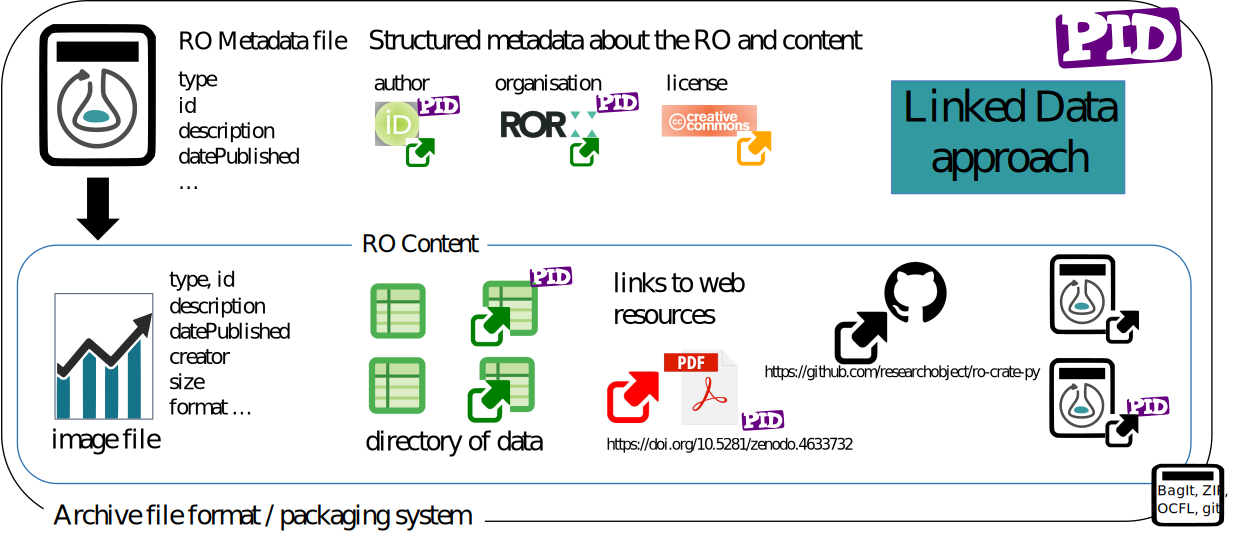
\includegraphics{content/images/ro-crate-overview.pdf}
\caption{Conceptual overview of RO-Crate. A \emph{Persistent
Identifier} (PID) \cite{doi:10.1371/journal.pbio.2001414} points to a
\emph{Research Object} (RO), which may be archived using different
packaging approaches like BagIt \cite{doi:10.17487/rfc8493}, OCFL \cite
{ocfl_2020}, git or ZIP. The RO is described within a \emph{RO-Crate
Metadata File}, providing identifiers for \emph{authors} using ORCID,
\emph{organisations} using Research Organization Registry (ROR) \cite
{doi:10.6087/kcse.192} and licences such as Creative Commons using SPDX
identifiers. The \emph{RO-Crate content} is further described with
additional metadata following a Linked Data approach. Data can be
embedded files and directories, as well as links to external Web
resources, PIDs and nested RO-Crates.}
\label{fig:conceptual}
\end{figure}

\subsubsection{Linked Data as a foundation}% {#linkeddata}

\label{sec:linkeddata}

The \textbf{Linked Data} principles \cite{doi:10.4018/978-1-60960-593-3.ch008}
(use of IRIs\footnote{\textbf{IRI}s \cite{doi:10.17487/rfc3987} are a generalisation
 of \textit{URI}s
(which include well-known http/https URLs), permitting international
Unicode characters without percent encoding, commonly used on the
browser address bar and in HTML5.} to identify resources (i.e. artefacts), resolvable via
HTTP, enriched with metadata and linked to each other) are core to
RO-Crate; therefore IRIs are used to identify an RO-Crate, its
constituent parts and metadata descriptions, and the properties and
classes used in the metadata.

RO-Crates are \textit{self-described} and follow the Linked Data principles to
describe all of their resources in both human and machine readable
manner. Hence, resources are identified using global identifiers
(absolute IRIs) where possible; and relationships between two resources
are defined with links.

The foundation of Linked Data and shared vocabularies also means that
multiple RO-Crates and other Linked Data resources can be indexed,
combined, queried, validated or transformed using existing Semantic Web
technologies such as SPARQL,\footnote{\url{https://www.w3.org/TR/sparql11-overview}}
SHACL\footnote{\url{https://www.w3.org/TR/shacl/}} and well established \textit{knowledge
graph} triple stores like Apache Jena\footnote{\url{https://jena.apache.org/}} and
OntoText GraphDB.\footnote{\url{https://www.ontotext.com/products/graphdb/}}

The possibilities of consuming\footnote{Some consideration is needed in processing of RO-Crates as
knowledge graphs, e.g. establishing absolute IRIs for files inside a
ZIP archive, detailed in the RO-Crate specification: \url
{https://www.researchobject.org/ro-crate/1.1/appendix/relative-uris.html}.} RO-Crate metadata with such
powerful tools gives another strong reason for using Linked Data as a
foundation. This use of mature Web\footnote{Note that an RO-Crate is not required to be published on the
Web, see Section~\ref{sec:selfdescribed}.} technologies also means its
developers and consumers are not restricted to the Research Object
aspects that have already been specified by the RO-Crate community, but
can extend and integrate RO-Crate in multiple standardised ways.

\subsubsection{RO-Crate is a self-described container}% {#selfdescribed}

\label{sec:selfdescribed}

An RO-Crate is defined\footnote{\url{https://www.researchobject.org/ro-crate/1.1/structure.html\#ro-crate-metadata-file-ro-crate-metadatajson}}
as a self-described \textbf{Root Data Entity} that describes and contains
\textit{data entities}, which are further described by referencing \textit{contextual
entities}. A \textbf{data entity} is either a \textit{file} (i.e. a byte sequence
stored on disk somewhere) or a \textit{directory} (i.e. set of named files and
other directories). A~file does not need to be stored inside the
RO-Crate root, it can be referenced via a PID/IRI. A \textbf{contextual
entity} exists outside the information system (e.g. a Person, a
workflow language) and is stored solely by its metadata. The
representation of a \textit{data entity} as a byte sequence makes it
possible to store a variety of research artefacts including not only
data but also, for instance, software and text.

The Root Data Entity is a directory, the \textit{RO-Crate Root}, identified by
the presence of the \textbf{RO-Crate Metadata File} \texttt{ro-crate-metadata.json}
(top of Fig.~\ref{fig:conceptual}). This file
describes the RO-Crate, its content and related metadata using Linked
Data in JSON-LD format \cite{sporny_2014}. This is a W3C standard RDF serialisation that has become
popular; it is easy to read by humans while also offering some
advantages for data exchange on the Internet. JSON-LD, a subset of the
widely supported and well-known JSON format, has tooling available for
many programming languages.\footnote{\url{https://json-ld.org/\#developers}}

The minimal requirements for the root data entity
metadata\footnote{\url{https://www.researchobject.org/ro-crate/1.1/root-data-entity.html\#direct-properties-of-the-root-data-entity}}
are \texttt{name}, \texttt{description} and \texttt{datePublished}, as well as a contextual
entity identifying its \texttt{license} -- additional metadata are commonly
added to entities depending on the purpose of the particular RO-Crate.

RO-Crates can be stored, transferred or published in multiple ways,
e.g. BagIt \cite{doi:10.17487/rfc8493}, Oxford Common File Layout
\cite{ocfl_2020} (OCFL), downloadable ZIP archives in Zenodo or through
dedicated online repositories, as well as published directly on the
Web, e.g. using GitHub Pages.\footnote{\url{https://pages.github.com/}} Combined
with Linked Data identifiers, this caters for a diverse set of storage
and access requirements across different scientific domains, from
metagenomics workflows producing hundreds of gigabytes of genome data
to cultural heritage records with access restrictions for personally
identifiable data. Specific \textit{RO-Crate profiles} (Section~\ref{sec:profiles}) may constrain serialization and publication
expectations, and require additional contextual types and properties.

\subsubsection{Data entities are described using contextual entities}% {#contextualentities}

\label{sec:contextualentities}

RO-Crate distinguishes between data and contextual
entities\footnote{\url{https://www.researchobject.org/ro-crate/1.1/contextual-entities.html\#contextual-vs-data-entities}}
in a similar way to HTTP terminology's early attempt to separate
\textit{information} (data) and \textit{non-information} (contextual) resources
\cite{httprange14}. Data entities are usually files and directories located
by relative IRI references within the RO-Crate Root, but they can also
be Web resources or restricted data identified with absolute IRIs,
including \textit{Persistent Identifiers} (PIDs) \cite{doi:10.1371/journal.pbio.2001414}.

As both types of entities are identified by IRIs, their distinction is
allowed to be blurry; data entities can be located anywhere and be
complex, while contextual entities can have a Web presence beyond their
description inside the RO-Crate. For instance
\texttt{https://orcid.org/0000-0002-1825-0097} is primarily an identifier for
a person, but secondarily it is also a Web page and a way to refer to
their academic work.

A particular IRI may appear as a contextual entity in one RO-Crate and
as a data entity in another; the distinction lies in the fact that data
entities can be considered to be \textit{contained} or captured by that
RO-Crate (\textit{RO Content} in Fig.~\ref{fig:conceptual}), while
contextual entities mainly \textit{explain} an RO-Crate or its content
(although this distinction is not a formal requirement).

In RO-Crate, a referenced contextual entity (e.g. a person identified
by ORCID) should always be described within the RO-Crate Metadata File
with at least a \textit{type} and \textit{name}, even where their PID might resolve
to further Linked Data. This is so that clients are not required to
follow every link for presentation purposes, for instance HTML
rendering. Similarly any imported extension
terms\footnote{\url{https://www.researchobject.org/ro-crate/1.1/appendix/jsonld.html\#extending-ro-crate}}
would themselves also have a human-readable description in the case
where their PID does not directly resolve to human-readable documentation.

Figure~\ref{fig:uml} shows a simplified UML class diagram of RO-Crate,
highlighting the different types of data entities and contextual
entities that can be aggregated and related. While an RO-Crate would
usually contain one or more data entities (\texttt{hasPart}), it may also be a
pure aggregation of contextual entities (\texttt{mentions}).

\begin{figure}%[t!]
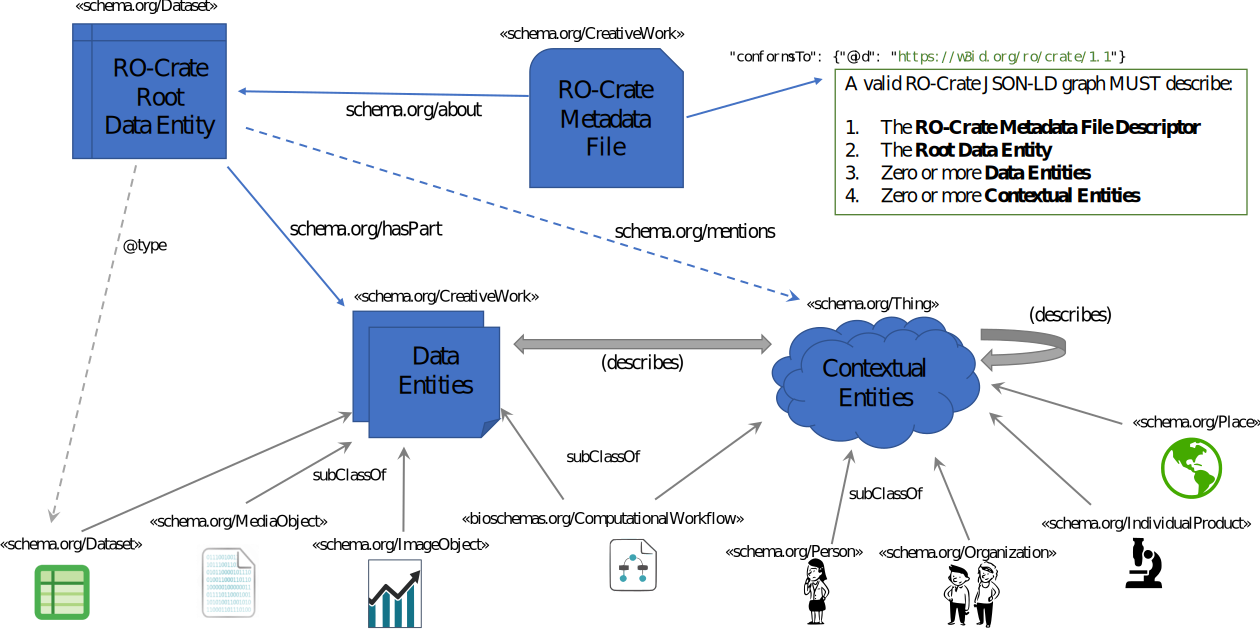
\includegraphics[width=0.9\textwidth]{content/images/ro-crate-uml.pdf}
\caption{Simplified UML class diagram of RO-Crate. The \emph
{RO-Crate Metadata File} conforms to a version of the specification;
and contains a JSON-LD graph \cite{sporny_2014} that describes the
entities that make up the RO-Crate. The \emph{RO-Crate Root Data
Entity} represent the Research Object as a dataset. The RO-Crate
aggregates \emph{data entities} (\texttt{hasPart}) which are further
described using \emph{contextual entities} (which may include
aggregated and non-aggregated data entities). Multiple types and
relations from Schema.org allow annotations to be more specific,
including figures, nested datasets, computational workflows, people,
organisations, instruments and places. Contextual entities not
otherwise cross-referenced from other entities' properties (\emph
{describes}) can be grouped under the root entity (\texttt{mentions}).}
\label{fig:uml}
\end{figure}

\subsubsection{Guide through recommended practices}% {#recommendedpractices}

\label{sec:recommendedpractices}

RO-Crate as a specification aims to build a set of recommended
practices on how to practically apply existing standards in a common
way to describe research outputs and their provenance, without having
to learn each of the underlying technologies in detail.

As such, the RO-Crate 1.1\footnote{\url{https://w3id.org/ro/crate/1.1}}
specification \cite{doi:10.5281/zenodo.4541002} can be seen as an
opinionated and example-driven guide to writing
Schema.org\footnote{\url{https://schema.org/}} \cite{doi:10.1145/2857274.2857276}
metadata as JSON-LD \cite{sporny_2014} (see Section~\ref{sec:implementation}), which leaves it open for implementers to include
additional metadata using other Schema.org types and properties, or
even additional Linked Data vocabularies/ontologies or their own ad-hoc terms.

However the primary purpose of the RO-Crate specification is to assist
developers in leveraging Linked Data principles for the focused purpose
of describing Research Objects in a structured language, while reducing
the steep learning curve otherwise associated with Semantic Web
adaptation, like development of ontologies, identifiers, namespaces,
and RDF serialization choices.
\subsubsection{Ensuring simplicity}% {#simplicity}

\label{sec:implicitly}

One aim of RO-Crate is to be conceptually simple. This simplicity has
been repeatedly checked and confirmed through an informal community
review process. For instance, in the discussion on supporting ad-hoc
vocabularies\footnote{\url{https://github.com/ResearchObject/ro-crate/issues/71}} in
RO-Crate, the community explored potential Linked Data solutions. The
conventional wisdom in RDF best
practices\footnote{\url{https://www.w3.org/TR/swbp-vocab-pub/}} is to establish a
vocabulary with a new IRI namespace, formalised using RDF
Schema\footnote{\url{http://www.w3.org/TR/2014/REC-rdf-schema-20140225/}} or
OWL\footnote{\url{http://www.w3.org/TR/2012/REC-owl2-overview-20121211/}}
ontologies. However, this may seem an excessive learning curve for
non-experts in semantic knowledge representation, and the RO-Crate
community instead agreed on a dual lightweight approach: (i)
Document\footnote{\url{https://www.researchobject.org/ro-crate/1.1/appendix/jsonld.html\#adding-new-or-ad-hoc-vocabulary-terms}}
how projects with their own Web-presence can make a pure HTML-based
vocabulary, and (ii) provide a community-wide PID namespace under
\texttt{https://w3id.org/ro/terms} that redirect to simple CSV files
maintained in GitHub.\footnote{\url{https://github.com/ResearchObject/ro-terms}}

To further verify this idea of simplicity, we have formalised the
RO-Crate definition (see \textit{Appendix~\ref{sec:formaldefinition}}). An
important result of this exercise is that the underlying data structure
of RO-Crate, although conceptually a graph, is represented as a
depth-limited tree. This formalisation also emphasises the
\textit{boundedness} of the structure; namely, the fact that elements are
specifically identified as being either semantically \textit{contained} by the
RO-Crate as \textit{Data Entities} (\texttt{hasPart}) or mainly referenced
(\texttt{mentions}) and typed as \textit{external} to the Research Object as
\textit{Contextual Entities}. It is worth pointing out that this semantic
containment can extend beyond the physical containment of files
residing within the RO-Crate Root directory on a given storage system,
as the RO-Crate data entities may include any data resource globally
identifiable using IRIs.
\subsubsection{Extensibility and RO-Crate profiles}% {#profiles}

\label{sec:profiles}

The RO-Crate specification provides a core set of conventions to
describe research outputs using types and properties applicable across
scientific domains. However we have found that domain-specific use of
RO-Crate will, implicitly or explicitly, form a specialised \textbf{profile}
of RO-Crate; i.e., {a set of conventions, types and properties that are
minimally required and one can expect to be present in that subset of
RO-Crates}. For instance, RO-Crates used for exchange of workflows will
have to contain a data entity of type \texttt{ComputationalWorkflow}, or
cultural heritage records should have a \texttt{contentLocation}.

Making such profiles explicit allow further reliable programmatic
consumption and generation of RO-Crates beyond the core types defined
in the RO-Crate specification. Following the RO-Crate mantra of
\textit{guidance over strictness}, profiles are mainly \textit{duck-typing} rather
than strict syntactic or semantic types, but may also have
corresponding machine-readable schemas at multiple levels (file
formats, JSON, RDF shapes, RDFS/OWL semantics).

The next version of the RO-Crate specification 1.2 will define a
formalization\footnote{\url{https://www.researchobject.org/ro-crate/1.2-DRAFT/profiles}}
for publishing and declaring conformance to RO-Crate profiles. Such a
profile is primarily a human-readable document of before-mentioned
expectations and conventions, but may also define a machine-readable
profile as a \textbf{Profile Crate}: Another RO-Crate that describe the
profile and in addition can list schemas for validation, compatible
software, applicable repositories, serialization/packaging formats,
extension vocabularies, custom JSON-LD contexts and examples (see for
example the Workflow RO-Crate
profile\footnote{\url{https://w3id.org/workflowhub/workflow-ro-crate/}}).

In addition, there are sometimes existing domain-specific metadata
formats, but they are either not RDF-based (and thus time-consuming to
construct terms for in JSON-LD) or are at a different granularity level
that might become overwhelming if represented directly in the RO-Crate
Metadata file (e.g. W3C PROV bundle detailing every step execution of a
workflow run \cite{doi:10.1093/gigascience/giz095}). RO-Crate allows such
\textit{alternative metadata files} to co-exist, and be described as data
entities with references to the standards and vocabularies they conform
to. This simplifies further programmatic consumption even where no
filename or file extension conventions have emerged for those metadata formats.

Section~\ref{sec:inuse} examines the observed specializations of
RO-Crate use in several domains and their emerging profiles.

\subsection{Technical implementation of the RO-Crate model}% {#implementation}

\label{sec:implementation}

The RO-Crate conceptual model has been realised using JSON-LD and
Schema.org in a prescriptive form as discussed in Section~\ref{sec:conceptual}. These technical choices were made to cater for
simplicity from a developer perspective (as introduced in Section~\ref{sec:methodology}).

JSON-LD\footnote{\url{https://json-ld.org/}} \cite{sporny_2014} provides a way to
express Linked Data as a JSON structure, where a \textit{context} provides
mapping to RDF properties and classes. While JSON-LD cannot map
arbitrary JSON structures to RDF, we found that it does lower the
barrier compared to other RDF syntaxes, as the JSON syntax nowadays is
a common and popular format for data exchange on the Web.

However, JSON-LD alone has too many degrees of freedom and hidden
complexities for software developers to reliably produce and consume
without specialised expertise or large RDF software frameworks. A large
part of the RO-Crate specification is therefore dedicated to describing
the acceptable subset of JSON structures.

\subsubsection{RO-Crate JSON-LD}% {#jsonld}

\label{sec:jsonld}

RO-Crate
mandates\footnote{\url{https://www.researchobject.org/ro-crate/1.1/appendix/jsonld.html}}
the use of flattened, compacted JSON-LD in the RO-Crate Metadata file
\texttt{ro-crate-metadata.json}\footnote{The avid reader may spot that the RO-Crate Metadata file use the
extension \texttt{.json} instead of \texttt{.jsonld}, this is to emphasise the
developer expectations as a JSON format, while the file's JSON-LD
nature is secondary. See \url
{https://github.com/ResearchObject/ro-crate/issues/82}.}
where a single \texttt{@graph} array contains all
the data and contextual entities in a flat list. An example can be seen
in the JSON-LD snippet in Listing \ref{lis1} below, describing a simple RO-Crate
containing data entities described using contextual entities.

\begin{listing}
%\includegraphics{210053i02}
\footnotesize
\begin{verbatim}
{ "@context": "https://w3id.org/ro/crate/1.1/context",
  "@graph": [
    { "@id": "ro-crate-metadata.json",      
      "@type": "CreativeWork",
      "conformsTo": {"@id": "https://w3id.org/ro/crate/1.1"},
      "about": {"@id": "./"}
    },
    { "@id": "./",
      "@type": "Dataset",
      "name": "A simplified RO-Crate",
      "author": {"@id": "#alice"},
      "license": {"@id": "https://spdx.org/licenses/CC-BY-4.0"},
      "datePublished": "2021-11-02T16:04:43Z",
      "hasPart": [
        {"@id": "survey-responses-2019.csv"},
        {"@id": "https://example.com/pics/5707039334816454031_o.jpg"}
      ]
    },
    { "@id": "survey-responses-2019.csv",
      "@type": "File",
      "about": {"@id": "https://example.com/pics/5707039334816454031_o.jpg"},
      "author": {"@id": "#alice"}
    },
    { "@id": "https://example.com/pics/5707039334816454031_o.jpg",
      "@type": ["File", "ImageObject"],
      "contentLocation": {"@id": "http://sws.geonames.org/8152662/"},
      "author": {"@id": "https://orcid.org/0000-0002-1825-0097"}
    },
    { "@id": "#alice",
      "@type": "Person",
      "name": "Alice"
    },
    { "@id": "https://orcid.org/0000-0002-1825-0097",
      "@type": "Person",
      "name": "Josiah Carberry"
    },
    { "@id": "http://sws.geonames.org/8152662/",
      "@type": "Place",
      "name": "Catalina Park"
    },
    { "@id": "https://spdx.org/licenses/CC-BY-4.0",
      "@type": "CreativeWork",
      "name": "Creative Commons Attribution 4.0"
    }
  ]
}    
\end{verbatim}    
\caption{%\qq{}\protect\footnotemark[31]
Simplified\protect\footnote{Recommended properties for types shown in
Listing \ref{lis1} also include
\texttt{affiliation}, \texttt{citation}, \texttt{contactPoint},
\texttt{description},
\texttt{encodingFormat}, \texttt{funder}, \texttt{geo}, \texttt{identifier},
\texttt{keywords},
\texttt{publisher}; these properties and corresponding contextual
entities are
excluded here for brevity. See complete example
\url
{https://www.researchobject.org/2021-packaging-research-artefacts-with-ro-crate/listing1/}.}
RO-Crate metadata file showing the
flattened compacted JSON-LD \texttt{@graph} array containing the data entities
and contextual entities, cross-referenced using \texttt{@id}. The
\texttt{ro-crate-metadata.json} entity self-declares conformance with the
RO-Crate specification using a versioned persistent identifier, further
RO-Crate descriptions are on the root data entity \texttt{./} or any of the
referenced data or contextual entities. This is exemplified by the data
entity \texttt{ImageObject} referencing contextual entities for
\texttt{contentLocation} and \texttt{author} that differs from that of the overall
RO-Crate. In this crate, \texttt{about} of the CSV data entity reference the
\texttt{ImageObject}, which then take the roles of both a data entity and
contextual entity. While \texttt{Person} entities ideally are identified with
ORCID PIDs as for Josiah, \texttt{\#alice} is here in contrast an RO-Crate
local identifier, highlighting the pragmatic ``just enough'' Linked
Data approach.}\label{lis1}
\end{listing}


In\footnotetext{Recommended properties for types shown in
Listing \ref{lis1} also include
\texttt{affiliation}, \texttt{citation}, \texttt{contactPoint},
\texttt{description},
\texttt{encodingFormat}, \texttt{funder}, \texttt{geo}, \texttt{identifier},
\texttt{keywords},
\texttt{publisher}; these properties and corresponding contextual
entities are
excluded here for brevity. See complete example
\url
{https://www.researchobject.org/2021-packaging-research-artefacts-with-ro-crate/listing1/}.} this flattened profile of JSON-LD, each \texttt{\{entity\}} is directly
under \texttt{@graph} and represents the RDF triples with a common \textit{subject}
(\texttt{@id}), mapped \textit{properties} like \texttt{hasPart}, and \textit{objects} -- as
either literal \texttt{"string"} values, referenced \texttt{\{objects\}} (which
properties are listed in its own entity), or a JSON \texttt{[list]} of these.
If processed as JSON-LD, this forms an RDF graph by matching the \texttt{@id}
IRIs and applying the \texttt{@context} mapping to Schema.org terms.
\normalsize

 \subsubsection{Flattened JSON-LD}

When JSON-LD 1.0 \cite{sporny_2014} was proposed, one of the motivations
was to seamlessly apply an RDF nature on top of regular JSON as
frequently used by Web APIs. JSON objects in APIs are frequently nested
with objects at multiple levels, and the perhaps most common form of
JSON-LD is the compacted
form\footnote{\url{https://json-ld.org/spec/REC/json-ld/20140116/\#compacted-document-form}}
which follows this expectation (JSON-LD
1.1\footnote{\url{https://www.w3.org/TR/2020/REC-json-ld11-20200716/}} further
expands these capabilities, e.g. allowing nested \texttt{@context} definitions).

While this feature of JSON-LD can be seen as a way to ``hide'' its RDF
nature, we found that the use of nested trees (e.g. a \texttt{Person} entity
appearing as \texttt{author} of a \texttt{File} which nests under a \texttt{Dataset} with
\texttt{hasPart}) counter-intuitively forces consumers to consider the JSON-LD
as an RDF Graph, since an identified \texttt{Person} entity can appear at
multiple and repeated points of the tree (e.g. author of multiple
files), necessitating node merging or duplication, which can become
complicated as this approach also invites the use of \textit{blank nodes}
(entities missing \texttt{@id}).

By comparison, a single flat \texttt{@graph} array approach, as required by
RO-Crate, means that applications can choose to process and edit each
entity as pure JSON by a simple lookup based on \texttt{@id}. At the same
time, lifting all entities to the same level reflects the Research
Object principles \cite{doi:10.1016/j.future.2011.08.004} in that
describing the context and provenance is just as important as
describing the data, and the requirement of \texttt{@id} of every entity
forces RO-Crate generators to consciously consider existing IRIs and
identifiers.\footnote{\url{https://www.researchobject.org/ro-crate/1.1/appendix/jsonld.html\#describing-entities-in-json-ld}}

\subsubsection{JSON-LD context}

In JSON-LD, the \texttt{@context} is a reference to another JSON-LD document
that provides mapping from JSON keys to Linked Data term IRIs, and can
enable various JSON-LD directives to cater for customised JSON
structures for translating to RDF.

RO-Crate reuses vocabulary terms and IRIs from Schema.org, but provides
its own versioned JSON-LD
context,\footnote{\url{https://w3id.org/ro/crate/1.1/context}} which has a flat list
with the mapping from JSON-LD keys to their IRI equivalents (e.g. key
\texttt{"author"} maps to the \url{http://schema.org/author} property).

The rationale behind this decision is to support JSON-based RO-Crate
applications that are largely unaware of JSON-LD, that still may want
to process the \texttt{@context} to find or add Linked Data definitions of
otherwise unknown properties and types. Not reusing the official
Schema.org context means RO-Crate is also able to map in additional
vocabularies where needed, namely the \textit{Portland Common Data Model}
(PCDM) \cite{pcdm} for repositories and Bioschemas \cite{bioschemas_2017} for
describing computational workflows. RO-Crate profiles may
extend\footnote{\url{https://www.researchobject.org/ro-crate/1.1/appendix/jsonld.html\#extending-ro-crate}}
the \texttt{@context} to re-use additional domain-specific ontologies.

Similarly, while the Schema.org context
currently\footnote{\url{https://schema.org/version/13.0/schemaorg-current-http.jsonld}}
have \texttt{"@type": "@id"} annotations for implicit object properties, RO-Crate
JSON-LD distinguishes explicitly between references to other entities
\texttt{\{"@id": "\#alice"}\}
and string values \texttt{"Alice"} -- meaning
RO-Crate applications can find references for corresponding entities
and IRIs without parsing the \texttt{@context} to understand a particular
property. Notably this is exploited by the \textit{ro-crate-html-js}
\cite{ro-crate-html-js} tool to provide reliable HTML rendering for
otherwise unknown properties and types.





\subsection{RO-Crate community}% {#community}

\label{sec:community}

The RO-Crate conceptual model, implementation and best practices are
developed by a growing community of researchers, developers and
publishers. RO-Crate's community is a key aspect of its effectiveness
in making research artefacts FAIR. Fundamentally, the community
provides the overall context of the implementation and model and
ensures its interoperability.

The RO-Crate community consists of:
\begin{enumerate}
\item[1.] a diverse set of people representing a variety of stakeholders;
\item[2.] a set of collective norms;
\item[3.] an open platform that facilitates communication (GitHub, Google
Docs, monthly teleconferences).
\end{enumerate}
\subsubsection{People}

The initial concept of RO-Crate was formed at the first Workshop on
Research Objects (RO2018\footnote{\url{https://www.researchobject.org/ro2018/}}),
held as part of the IEEE conference on eScience. This workshop followed
up on considerations made at a Research Data Alliance (RDA) meeting on
Research Data
Packaging\footnote{\url{https://rd-alliance.org/approaches-research-data-packaging-rda-11th-plenary-bof-meeting}}
that found similar goals across multiple data packaging efforts
\cite{doi:10.5281/zenodo.3250687}: simplicity, structured metadata and the
use of JSON-LD.

An important outcome of discussions that took place at RO2018 was the
conclusion that the original Wf4Ever Research Object ontologies
\cite{doi:10.1016/j.websem.2015.01.003}, in principle sufficient for
packaging research artefacts with rich descriptions, were, in practice,
considered inaccessible for regular programmers (e.g., Web developers)
and in danger of being incomprehensible for domain scientists due to
their reliance on Semantic Web technologies and other ontologies.

DataCrate \cite{doi:10.5281/zenodo.1445817} was presented at RO2018 as a
promising lightweight alternative approach, and an agreement was made
by a group of volunteers to attempt building what was initially called
\textit{``RO Lite''} as a combination of DataCrate's implementation and
Research Object's principles.

This group, originally made up of library and Semantic Web experts, has
subsequently grown to include domain scientists, developers, publishers
and more. This perspective of multiple views led to the specification
being used in a variety of domains, from bioinformatics and regulatory
submissions to humanities and cultural heritage preservation.

The RO-Crate community is strongly engaged with the European-wide
biology/bioinformatics collaborative e-Infrastructure ELIXIR
\cite{doi:10.1016/j.tibtech.2012.02.002}, along with European Open Science
Cloud\footnote{\url{https://eosc.eu/}} (EOSC) projects including
EOSC-Life,\footnote{\url{https://www.eosc-life.eu/}}
FAIRplus,\footnote{\url{https://fairplus-project.eu/}}
CS3MESH4EOSC\footnote{\url{https://cs3mesh4eosc.eu/}} and
BY-COVID.\footnote{\url{https://by-covid.eu/}} RO-Crate has also established
collaborations with Bioschemas \cite{bioschemas_2017}, GA4GH
\cite{doi:10.1016/j.xgen.2021.100029}, OpenAIRE \cite{rettberg_2015_openaire}
and multiple H2020 projects.

A key set of stakeholders are developers: the RO-Crate community has
made a point of attracting developers who can implement the
specifications but, importantly, keeps ``developer user experience'' in
mind. This means that the specifications are straightforward to
implement and thus do not require expertise in technologies that are
not widely deployed.

This notion of catering to ``developer user experience'' is an example
of the set of norms that have developed and now define the community.

\subsubsection{Norms}

The RO-Crate community is driven by informal conventions and notions
that are prevalent but not neccessarily written down. Here, we distil
what we as authors believe are the critical set of norms that have
facilitated the development of RO-Crate and contributed to the ability
for RO-Crate research packages to be FAIR. This is not to say that
there are no other norms within the community nor that everyone in the
community holds these uniformly. Instead, what we emphasise is that
these norms are helpful and also shaped by community practices.
\begin{enumerate}
\item[1.] Simplicity
\item[2.] Developer friendliness
\item[3.] Focus on examples and best practices rather than rigorous specification
\item[4.] Reuse ``just enough'' Web standards
\end{enumerate}

A core norm of RO-Crate is that of \textbf{simplicity}, which sets the scene
for how we guide developers to structure metadata with RO-Crate. We
focus mainly on documenting simple approaches to the most common use
cases, such as authors having an affiliation. This norm also influences
our take on \textbf{developer friendliness}; for instance, we are using the
Web-native JSON format, allowing only a few of JSON-LD's flexible
Linked Data features. Moreover, the RO-Crate documentation is largely
built up by \textbf{examples} showcasing \textbf{best practices}, rather than
rigorous specifications. We build on existing \textbf{Web standards} that
themselves are defined rigorously, which we utilise \textit{``\textbf{just
enough}''} in order to benefit from the advantages of Linked Data
(e.g., extensions by namespaced vocabularies), without imposing too
many developer choices or uncertainties (e.g., having to choose between
the many RDF syntaxes).

While the above norms alone could easily lead to the creation of ``yet
another'' JSON format, we keep the goal of \textbf{FAIR interoperability} of
the captured metadata, and therefore follow closely FAIR best practices
and current developments such as data citations, PIDs, open
repositories and recommendations for sharing research outputs and software.

\subsubsection{Open platforms}

The critical infrastructure that enables the community around RO-Crate
is the use of open development platforms. This underpins the importance
of open community access to supporting FAIR. Specifically, it is
difficult to build and consume FAIR research artefacts without being
able to access the specifications, understand how they are developed,
know about any potential implementation issues, and discuss usage to
evolve best practices.

The development of RO-Crate was driven by capturing documentation of
real-life examples and best practices rather than creating a rigorous
specification. At the same time, we agreed to be opinionated on the
syntactic form to reduce the jungle of implementation choices; we
wanted to keep the important aspects of Linked Data to adhere to the
FAIR principles while retaining the option of combining and extending
the structured metadata using the existing Semantic Web stack, not just
build a standalone JSON format.

Further work during 2019 started adapting the DataCrate documentation
through a more collaborative and exploratory \textit{RO Lite} phase, initially
using Google Docs for review and discussion, then moving to GitHub as a
collaboration space for developing what is now the RO-Crate
specification, maintained\footnote{\url{https://github.com/researchobject/ro-crate/}} as
Markdown in GitHub Pages
and published through Zenodo.

In addition to the typical Open Source-style development with GitHub
issues and pull requests, the RO-Crate Community have, at time of
writing, two regular monthly calls, a Slack channel and a mailing list
for coordinating the project; also many of its participants collaborate
on RO-Crate at multiple conferences and coding events such as the
ELIXIR BioHackathon.\footnote{\url{https://biohackathon-europe.org/}} The community
is jointly developing the RO-Crate specification and Open Source tools,
as well as providing support and considering new use cases. The
RO-Crate Community\footnote{\url{https://www.researchobject.org/ro-crate/community}}
is open for anyone to join, to equally participate under a code of
conduct, and as of October 2021 has more than 50 members (see Appendix~\ref{sec:communitylist}).

% Please update in 31.tooling-table.md first!
%
\begin{table}[t!]%[htbp]
\tabcolsep=0pt
\caption{Applications and libraries implementing RO-Crate, targeting
different types of users across multiple programming languages. Status
is indicative as assessed by this work (Alpha $<$ Beta $<$ Release
Candidate (RC) $<$ Release)}
\label{tab1}
%
\begin{tabular*}{\textwidth}{@{\extracolsep{4in minus 4in}}llcc@{}}
\hline
\textbf{Tool name} & \multicolumn{1}{c}{\tmultirow{2}{*}{Targets}}
& \tmultirow{2}{*}{Language/Platform} & \tmultirow{2}{*}{Status} \\
\textit{Brief Description}&&& \\
\hline
\textbf{Describo} \cite{describo}                                                                                                          & Research Data Managers     & NodeJS (Desktop) & RC    \\
\multicolumn{4}{@{}l@{}}{\textit{Interactive desktop application to create, update and export RO-Crates for different profiles}}                                                                               \\
\textbf{Describo Online} \cite{describo-online}                                                                                            & Platform developers        & NodeJS (Web)     & Alpha \\
\multicolumn{4}{@{}l@{}}{\textit{Web-based application to create RO-Crates using cloud storage}}                                                                                                               \\
\textbf{ro-crate-excel} \cite{ro-crate-excel}                                                                                              & Data managers              & JavaScript       & Beta  \\
\multicolumn{4}{@{}l@{}}{\textit{Command-line tool to create/edit RO-Crates with spreadsheets}}                                                                                                                \\
\textbf{ro-crate-html-js} \cite{ro-crate-html-js}                                                                                          & Developers                 & JavaScript       & Beta  \\
\multicolumn{4}{@{}l@{}}{\textit{HTML rendering of RO-Crate}}                                                                                                                                                  \\
\textbf{ro-crate-js} \cite{ro-crate-js}                                                                                                    & Research Data Managers     & JavaScript       & Alpha \\
\multicolumn{4}{@{}l@{}}{\textit{Library for creating/manipulating crates; basic validation code}}                                                                                                             \\
\textbf{ro-crate-ruby} \cite{ro-crate-ruby}                                                                                                & Developers                 & Ruby             & Beta  \\
\multicolumn{4}{@{}l@{}}{\textit{Ruby library for reading/writing RO-Crate, with workflow support}}                                                                                                            \\
\textbf{ro-crate-py} \cite{ro-crate-py}                                                                                                    & Developers                 & Python           & Beta  \\
\multicolumn{4}{@{}l@{}}{\textit{Object-oriented Python library for reading/writing RO-Crate and use by Jupyter Notebook}}                                                                                     \\
\textbf{WorkflowHub} \cite{about-workflowhub}                                                                                              & Workflow users             & Ruby             & Beta  \\
\multicolumn{4}{@{}l@{}}{\textit{Workflow repository; imports and exports Workflow RO-Crate}}                                                                                                                  \\
\textbf{Life Monitor} \cite{about-lifemonitor}                                                                                             & Workflow developers        & Python           & Alpha \\
\multicolumn{4}{@{}l@{}}{\textit{Workflow testing and monitoring service; Workflow Testing profile of RO-Crate}}                                                                                               \\
\textbf{SCHeMa} \cite{vergoulis2021schema}                                                                                                 & Workflow users             & PHP              & Alpha \\
\multicolumn{4}{@{}l@{}}{\textit{Workflow execution using RO-Crate as exchange mechanism}}                                                                                                                     \\
\textbf{galaxy2cwl} \cite{galaxy2cwl}                                                                                                      & Workflow developers        & Python           & Alpha \\
\multicolumn{4}{@{}l@{}}{\textit{Wraps Galaxy workflow as Workflow RO-Crate}}                                                                                                                                  \\
\textbf{Modern PARADISEC} \cite{modpdsc}                                                                                                   & Repository managers        & Platform         & Beta  \\
\multicolumn{4}{@{}l@{}}{\textit{Cultural Heritage portal based on OCFL and RO-Crate}}                                                                                                                        \\
\textbf{ONI express} \cite{arkisto-data-portal}                                                                                            & Repository managers        & Platform         & Beta  \\
\multicolumn{4}{@{}l@{}}{\textit{Platform for publishing data and documents stored in an OCFL repository via a Web interface}}                                                                                 \\
\textbf{ocfl-tools} \cite{ocfl-tools}                                                                                                      & Developers                 & JavaScript (CLI) & Beta  \\
\multicolumn{4}{@{}l@{}}{\textit{Tools for managing RO-Crates in an OCFL repository}}                                                                                                                          \\
\textbf{RO Composer} \cite{ro-composer}                                                                                                    & Repository developers      & Java             & Alpha \\
\multicolumn{4}{@{}l@{}}{\textit{REST API for gradually building ROs for given profile}}                                                                                                                       \\
\textbf{RDA maDMP Mapper} \cite{doi:10.5281/zenodo.3922136}                                                                                & Data Management Plan users & Python           & Beta  \\
\multicolumn{4}{@{}l@{}}{\textit{Mapping between machine-actionable data management plans (maDMP) and RO-Crate \cite{doi:10.4126/frl01-006423291}}}                                                         \\
\textbf{Ro-Crate\_2\_ma-DMP} \cite{doi:10.5281/zenodo.3903463}                                                                             & Data Management Plan users & Python           & Beta  \\
\multicolumn{4}{@{}l@{}}{\textit{Convert between machine-actionable data management plans (maDMP) and RO-Crate}}                                                                                              \\
\textbf{CheckMyCrate} \cite{CheckMyCrate}                                                                                                  & Developers                 & Python (CLI)     & Alpha \\
\multicolumn{4}{@{}l@{}}{\textit{Validation according to Workflow RO-Crate profile}}                                                                                                                           \\
\textbf{RO-Crates-and-Excel} \cite{doi:10.5281/zenodo.5068950}                                                                             & Data Managers              & Java (CLI)       & Alpha \\
\multicolumn{4}{@{}l@{}}{\textit{Describe column/data details of spreadsheets as RO-Crate using DataCube vocabulary}}                                                                                          \\
\hline
\end{tabular*}\vspace*{10pt}
\end{table}


\section{RO-Crate tooling}% {#tooling}

\label{sec:tooling}

The work of the community has led to the development of a number of
tools for creating and using RO-Crates. Table~\ref{tab1} shows the current set
of implementations. Reviewing this list, one can see support for
commonly used programming languages, including Python, JavaScript, and
Ruby. Additionally, the tools can be integrated into commonly used
research environments, in particular, the command line tool
\textit{ro-crate-html-js} \cite{ro-crate-html-js} for creating a human-readable
preview of an RO-Crate as a sidecar HTML file. Furthermore, there are
tools that cater to end-users (\textit{Describo} \cite{describo}, \textit{WorkflowHub}
\cite{about-workflowhub}), in order to simplify creating and managing
RO-Crate. For example, Describo was developed to help researchers of
the Australian Criminal Characters
project\footnote{\url{https://criminalcharacters.com/}} to annotate historical prisoner
records for greater insight into the history of Australia
\cite{doi:10.1080/14490854.2020.1796500}.

While the development of these tools is promising, our analysis of
their maturity status shows that the majority of them are in the Beta
stage. This is partly due to the fact that the RO-Crate specification
itself only recently reached 1.0 status, in November 2019
\cite{doi:10.5281/zenodo.3541888}. Now that there is a fixed point of
reference: With version 1.1 (October 2020)
\cite{doi:10.5281/zenodo.4031327} RO-Crate has stabilised based on feedback
from application development, and now we are seeing a further increase
in the maturity of these tools, along with the creation of new ones.

Given the stage of the specification, these tools have been primarily
targeting developers, essentially providing them with the core
libraries for working with RO-Crate. Another target has been that of
research data managers who need to manage and curate large amounts of data.

\section{Profiles of RO-Crate in use}% {#inuse}

\label{sec:inuse}

RO-Crate fundamentally forms part of an infrastructure to help build
FAIR research artefacts. In other words, the key question is whether
RO-Crate can be used to share and (re)use research artefacts. Here we
look at three research domains where RO-Crate is being applied:
Bioinformatics, Regulatory Science and Cultural Heritage. In addition,
we note how RO-Crate may have an important role as part of
machine-actionable data management plans and institutional repositories.

From these varied uses of RO-Crate we observe natural differences in
their detail level and the type of entities described by the RO-Crate.
For instance, on submission of an RO-Crate to a workflow repository, it
is reasonable to expect the RO-Crate to contain at least one workflow,
ideally with a declared licence and workflow language. Specific
additional recommendations such as on identifiers is also needed to
meet the emerging requirements of FAIR Digital
Objects.\footnote{\url{https://fairdo.org/}} Work has now
begun\footnote{\url{https://github.com/ResearchObject/ro-crate/issues/153}} to
formalise these different \textit{profiles} of RO-Crates, which may impose
additional constraints based on the needs of a specific domain or use case.

\subsection{Bioinformatics workflows}% {#workflows}

\label{sec:workflows}

WorkflowHub.eu\footnote{\url{https://workflowhub.eu/}} is a European cross-domain
registry of computational workflows, supported by European Open Science
Cloud projects, e.g. EOSC-Life,\footnote{\url{https://www.eosc-life.eu/}} and
research infrastructures including the pan-European bioinformatics
network ELIXIR\footnote{\url{https://elixir-europe.org/}}
\cite{doi:10.1016/j.tibtech.2012.02.002}. As part of promoting workflows as
reusable tools, WorkflowHub includes documentation and high-level
rendering of the workflow structure independent of its native workflow
definition format. The rationale is that a domain scientist can browse
all relevant workflows for their domain, before narrowing down their
workflow engine requirements. As such, the WorkflowHub is intended
largely as a registry of workflows already deposited in repositories
specific to particular workflow languages and domains, such as
UseGalaxy.eu \cite{doi:10.1371/journal.ppat.1008643} and Nextflow nf-core
\cite{doi:10.1038/s41587-020-0439-x}.

We here describe three different RO-Crate profiles developed for use
with WorkflowHub.

\subsubsection{Profile for describing workflows}

Being cross-domain, WorkflowHub has to cater for many different
workflow systems. Many of these, for instance Nextflow
\cite{doi:10.1038/nbt.3820} and Snakemake
\cite{doi:10.1093/bioinformatics/bts480}, by virtue of their script-like
nature, reference multiple neighbouring files typically maintained in a
GitHub repository. This calls for a data exchange method that allows
keeping related files together. WorkflowHub has tackled this problem by
adopting RO-Crate as the packaging mechanism
\cite{doi:10.5281/zenodo.4705078}, typing and annotating the constituent
files of a workflow and -- crucially -- marking up the workflow
language, as many workflow engines use common file extensions like
\texttt{*.xml} and \texttt{*.json}. Workflows are further described with authors,
license, diagram previews and a listing of their inputs and outputs.
RO-Crates can thus be used for interoperable deposition of workflows to
WorkflowHub, but are also used as an archive for downloading workflows,
embedding metadata registered with the WorkflowHub entry and translated
workflow files such as abstract Common Workflow Language (CWL)
\cite{doi:10.1145/3486897} definitions and diagrams \cite{doi:10.5281/zenodo.4605654}.

RO-Crate acts therefore as an interoperability layer between
registries, repositories and users in WorkflowHub. The iterative
development between WorkflowHub developers and the RO-Crate community
heavily informed the creation of the Bioschemas \cite{bioschemas_2017}
profile for Computational
Workflows,\footnote{\url{https://bioschemas.org/profiles/ComputationalWorkflow/1.0-RELEASE/}}
which again informed the RO-Crate 1.1 specification on
workflows\footnote{\url{https://www.researchobject.org/ro-crate/1.1/workflows.html}}
and led to the RO-Crate Python library \cite{ro-crate-py} and WorkflowHub's
\textbf{Workflow RO-Crate
profile},\footnote{\url{https://w3id.org/workflowhub/workflow-ro-crate/1.0}} which,
in a similar fashion to RO-Crate itself, recommends which workflow
resources and descriptions are required. This co-development across
project boundaries exemplifies the drive for simplicity and for
establishing best practices.

\subsubsection{Profile for recording workflow runs}

RO-Crates in WorkflowHub have so far been focused on workflows that are
ready to be run, and development of WorkflowHub is now creating a
\textbf{Workflow Run RO-Crate profile} for the purposes of benchmarking,
testing and executing workflows. As such, RO-Crate serves as a
container of both a \textit{workflow definition} that may be executed and of a
particular \textit{workflow execution with test results}.

This workflow run profile is a continuation of our previous work with
capturing workflow provenance in a Research Object in CWLProv
\cite{doi:10.1093/gigascience/giz095} and TavernaPROV
\cite{doi:10.5281/zenodo.51314}. In both cases, we used the PROV Ontology
\cite{PROVO}, including details of every task execution with all the
intermediate data, which required significant workflow engine
integration.\footnote{CWLProv and TavernaProv predate RO-Crate, but use
RO-Bundle\cite{doi:10.5281/zenodo.12586}, a similar Research Object
packaging method with JSON-LD metadata.}

Simplifying from the CWLProv approach, the planned Workflow Run
RO-Crate profile will use a high level Schema.org
provenance\footnote{\url{https://www.researchobject.org/ro-crate/1.1/provenance.html\#software-used-to-create-files}}
for the input/output boundary of the overall workflow execution. This
\textit{Level 1 workflow provenance} \cite{doi:10.1093/gigascience/giz095} can be
expressed generally across workflow languages with minimal workflow
engine changes, with the option of more detailed provenance traces as
separate PROV artefacts in the RO-Crate as data entities. In the
current development of Specimen Data
Refinery\footnote{\url{https://github.com/DiSSCo/SDR}} \cite{doi:10.3897/rio.6.e57602}
these RO-Crates will document the text recognition workflow runs of
digitised biological specimens, exposed as FAIR Digital Objects
\cite{doi:10.3390/publications8020021}.

WorkflowHub has recently enabled minting of Digital Object Identifiers
(DOIs), a PID commonly used for scholarly artefacts, for registered
workflows, e.g. \texttt{10.48546/workflowhub.workflow.56.1}
\cite{doi:10.48546/workflowhub.workflow.56.1}, lowering the barrier for
citing workflows as computational methods along with their FAIR
metadata -- captured within an RO-Crate. While it is not an aim for
WorkflowHub to be a repository of workflow runs and their data,
RO-Crates of \textit{exemplar workflow runs} serve as useful workflow
documentation, as well as being an exchange mechanism that preserves
FAIR metadata in a diverse workflow execution environment.

\subsubsection{Profile for testing workflows}

The value of computational workflows, however, is potentially
undermined by the ``collapse'' over time of the software and services
they depend upon: for instance, software dependencies can change in a
non-backwards-compatible manner, or active maintenance may cease; an
external resource, such as a reference index or a database query
service, could shift to a different URL or modify its access protocol;
or the workflow itself may develop hard-to-find bugs as it is updated.
This \textit{workflow decay} can take a big toll on the workflow's reusability
and on the reproducibility of any processes it evokes
\cite{doi:10.1109/eScience.2012.6404482}.

For this reason, WorkflowHub is complemented by a monitoring and
testing service called LifeMonitor \cite{about-lifemonitor}, also supported
by EOSC-Life. LifeMonitor's main goal is to assist in the creation,
periodic execution and monitoring of workflow tests, enabling the early
detection of software collapse in order to minimise its detrimental
effects. The communication of metadata related to workflow testing is
achieved through the adoption of a \textbf{Workflow Testing RO-Crate
profile}\footnote{\url{https://lifemonitor.eu/workflow_testing_ro_crate}} stacked on
top of the \textit{Workflow RO-Crate} profile. This further specialisation of
Workflow RO-Crate allows to specify additional testing-related entities
(test suites, instances, services, etc.), leveraging RO-Crate's
extension
mechanism\footnote{\url{https://www.researchobject.org/ro-crate/1.1/appendix/jsonld.html\#extending-ro-crate}}
through the addition of terms from custom namespaces.

In addition to showcasing RO-Crate's extensibility, the testing profile
is an example of the format's flexibility and adaptability to the
different needs of the research community. Though ultimately related to
a computational workflow, in fact, most of the testing-specific
entities are more about describing a protocol for interacting with a
monitoring service than a set of research outputs and its associated
metadata. Indeed, one of LifeMonitor's main functionalities is
monitoring and reporting on test suites running on existing Continuous
Integration (CI) services, which is described in terms of service URLs
and job identifiers in the testing profile. In principle, in this
context, data could disappear altogether, leading to an RO-Crate
consisting entirely of contextual entities. Such an RO-Crate acts more
as an exchange format for communication between services (WorkflowHub
and LifeMonitor) than as an aggregator for research data and metadata,
providing a good example of the format's high versatility.


\subsection{Regulatory sciences}% {#regulatorysciences}

\label{sec:regulatorysciences}

BioCompute Objects\footnote{\url{https://biocomputeobject.org/}} (BCO)
\cite{doi:10.1371/journal.pbio.3000099} is a community-led effort to
standardise submissions of computational workflows to biomedical
regulators. For instance, a genomics sequencing pipeline, as part of a
personalised cancer treatment study, can be submitted to the US Food
and Drugs Administration (FDA) for approval. BCOs are formalised in the
standard IEEE 2791-2020 \cite{doi:10.1109/IEEESTD.2020.9094416} as a
combination of JSON
Schemas\footnote{\url{https://w3id.org/ieee/ieee-2791-schema/}}
that define the structure of JSON metadata files describing exemplar
workflow runs in detail, covering aspects such as the usability and
error domain of the workflow, its runtime requirements, the reference
datasets used and representative output data produced.

BCOs provide a structured view over a particular workflow, informing
regulators about its workings independently of the underlying workflow
definition language. However, BCOs have only limited support for
additional metadata.\footnote{IEEE 2791-2020 do permit user extensions in the \textit{extension
domain} by referencing additional JSON Schemas.} For instance, while the BCO itself can
indicate authors and contributors, and in particular regulators and
their review decisions, it cannot describe the provenance of individual
data files or workflow definitions.

As a custom JSON format, BCOs cannot be extended with Linked Data
concepts, except by adding an additional top-level JSON object
formalised in another JSON Schema. A BCO and workflow submitted by
upload to a regulator will also frequently consist of multiple
cross-related files. Crucially, there is no way to tell whether a given
\texttt{*.json} file is a BCO file, except by reading its content and check
for its \texttt{spec\_version}.

We can then consider how a BCO and its referenced artefacts can be
packaged and transferred following FAIR principles. \textbf{BCO
RO-Crate}\footnote{\url{https://biocompute-objects.github.io/bco-ro-crate/}} \cite{doi:10.5281/zenodo.4633732},
part of the BioCompute Object user guides, defines a set of best
practices for wrapping a BCO with a workflow, together with its
exemplar outputs in an RO-Crate, which then provides typing and
additional provenance metadata of the individual files, workflow
definition, referenced data and the BCO metadata itself.

Here the BCO is responsible for describing the \textit{purpose} of a workflow
and its run at an abstraction level suitable for a domain scientist,
while the more open-ended RO-Crate describes the surroundings of the
workflow, classifying and relating its resources and providing
provenance of their existence beyond the BCO. This emerging \textit{separation
of concerns} is shown in Fig.~\ref{fig:sep_concerns}, and highlights
how RO-Crate is used side-by-side of existing standards and tooling,
even where there are apparent partial overlaps.

A similar separation of concerns can be found if considering the
RO-Crate as a set of files, where the \textit{transport-level} metadata, such
as checksum of files, are delegated to separate
BagIt\footnote{\url{https://www.researchobject.org/ro-crate/1.1/appendix/implementation-notes.html\#adding-ro-crate-to-bagit}}
manifests, a standard focusing on the preservation challenges of
digital libraries \cite{doi:10.17487/rfc8493}. As such, RO-Crate metadata
files are not required to iterate all the files in their folder
hierarchy, only those that benefit from being described.

Specifically, a BCO description alone is insufficient for reliable
re-execution of a workflow, which would need a compatible workflow
engine depending on the original workflow definition language, so IEEE
2791 recommends using Common Workflow Language (CWL)
\cite{doi:10.1145/3486897} for interoperable pipeline execution. CWL itself
relies on tool packaging in software containers using
Docker\footnote{\url{https://www.docker.com/}} or Conda.\footnote{\url{https://docs.conda.io/}}
Thus, we can consider BCO RO-Crate as a stack: transport-level
manifests of files (BagIt), provenance, typing and context of those
files (RO-Crate), workflow overview and purpose (BCO), interoperable
workflow definition (CWL) and tool distribution (Docker).

%
\begin{figure}%[t]
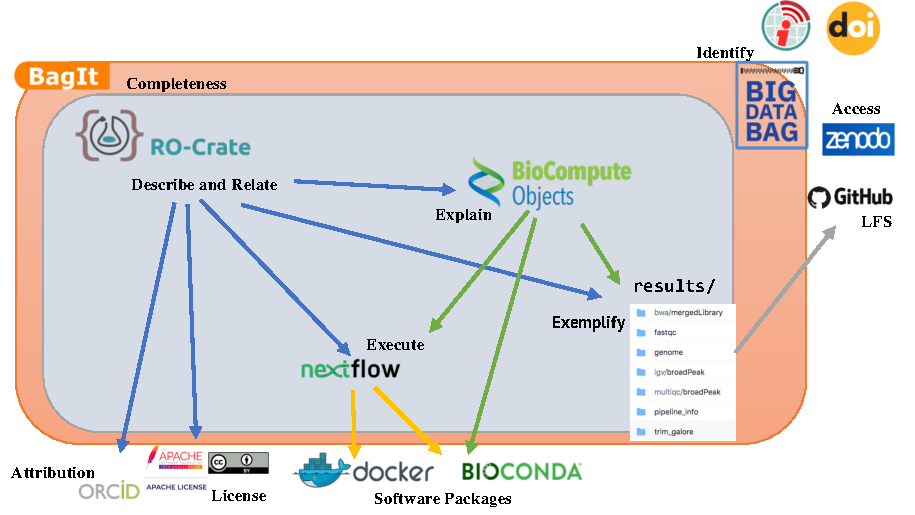
\includegraphics{content/images/ro-crate-bco-sep-of-concerns.pdf}
\caption{Separation of Concerns in BCO RO-Crate. BioCompute
Object (IEEE2791) is a JSON file that structurally explains the purpose
and implementation of a computational workflow, for instance
implemented in Common Workflow Language (CWL), that installs the
workflow's software dependencies as Docker containers or BioConda
packages. An example execution of the workflow shows the different
kinds of result outputs, which may be external, using GitHub LFS \cite
{github-lfs} to support larger data. RO-Crate gathers all these local
and external resources, relating them and giving individual
descriptions, for instance permanent DOI identifiers for reused
datasets accessed from Zenodo, but also adding external identifiers to
attribute authors using ORCID or to identify which licences apply to
individual resources. The RO-Crate and its local files are captured in
a BagIt whose checksum ensures completeness, combined with Big Data Bag
\cite{doi:10.1109/BigData.2016.7840618} features to ``complete'' the
bag with large external files such as the workflow outputs.}
\label{fig:sep_concerns}
\end{figure}
%
\subsection{Digital humanities: Cultural heritage}% {#culturalheritage}

\label{sec:culturalheritage}

The Pacific And Regional Archive for Digital Sources in Endangered
Cultures (PARADISEC\footnote{\url{https://www.paradisec.org.au/}}) \cite{doi:10125/4567}
maintains a repository of more than 500,000 files documenting
endangered languages across more than 16,000 items, collected and
digitised over many years by researchers interviewing and recording
native speakers across the region.

The Modern PARADISEC demonstrator\footnote{\url{https://mod.paradisec.org.au/}} has
been
proposed\footnote{\url{https://arkisto-platform.github.io/case-studies/paradisec/}}
as an update to the 18 year old infrastructure, to also help long-term
preservation of these artefacts in their digital form. The demonstrator
uses RO-Crate to describe the overall structure and to capture the
metadata of each item. The existing PARADISEC data collection has been
ported and captured as RO-Crates. A Web portal then exposes the
repository and its entries by indexing the RO-Crate metadata files,
presenting a domain-specific view of the items -- the RO-Crate is
``hidden'' and does not change the user interface.

The PARADISEC use case takes advantage of several RO-Crate features and
principles. Firstly, the transcribed metadata are now independent of
the PARADISEC platform and can be archived, preserved and processed in
its own right, using Schema.org as base vocabulary and extended with
PARADISEC-specific terms.

In this approach, RO-Crate is the holder of itemised metadata, stored
in regular files that are organised using Oxford Common File
Layout\footnote{\url{https://ocfl.io/1.0/spec/}} (OCFL) \cite{ocfl_2020}, which ensures
file integrity and versioning on a regular shared file system. This
lightweight infrastructure also gives flexibility for future
developments and maintenance. For example a consumer can use Linked
Data software such as a graph database and query the whole corpora
using SPARQL triple patterns across multiple RO-Crates. For long term
digital preservation, beyond the lifetime of PARADISEC portals, a
``last resort'' fallback is storing the generic RO-Crate HTML preview
\cite{ro-crate-html-js}. Such human-readable rendering of RO-Crates can be
hosted as static files by any Web server, in line with the approach
taken by the Endings Project.\footnote{The Endings Project \url{https://endings.uvic.ca/} is a five-year
project funded by the Social Sciences and Humanities Research Council
(SSHRC) that is creating tools, principles, policies and
recommendations for digital scholarship practitioners to create
accessible, stable, long-lasting resources in the humanities.}

\subsection{Machine-actionable Data Management Plans}% {#dmp}

\label{sec:dmp}

Machine-actionable Data Management Plans (maDMPs) have been proposed as
an improvement to automate FAIR data management tasks in research
\cite{doi:10.1371/journal.pcbi.1006750}; maDMPs use PIDs and controlled
vocabularies to describe what happens to data over the research life
cycle \cite{doi:10.1007/978-3-030-45442-5_15}. The Research Data Alliance's
\textit{DMP Common Standard} for maDMPs \cite{doi:10.15497/rda00039} is one such
formalisation for expressing maDMPs, which can be expressed as Linked
Data using the DMP Common Standard Ontology
\cite{doi:10.4126/frl01-006423289}, a specialisation of the W3C Data
Catalog Vocabulary (DCAT) \cite{dcat2}. RDA maDMPs are usually expressed
using regular JSON, conforming to the DMP JSON Schema.

A mapping has been produced between Research Object Crates and
Machine-actionable Data Management Plans
\cite{doi:10.4126/frl01-006423291}, implemented by the RO-Crate RDA maDMP
Mapper \cite{doi:10.5281/zenodo.3922136}. A similar mapping has been
implemented by \textit{RO-Crate\_2\_ma-DMP} \cite{doi:10.5281/zenodo.3903463}. In
both cases, a maDMP can be converted to a RO-Crate, or vice versa. In
\cite{doi:10.4126/frl01-006423291} this functionality caters for two use cases:
\begin{enumerate}
\item[1.] Start a skeleton data management plan based on an existing RO-Crate
dataset, e.g. an RO-Crate from WorkflowHub.
\item[2.] Instantiate an RO-Crate based on a data management plan.
\end{enumerate}

An important nuance here is that data management plans are (ideally)
written in \textit{advance} of data production, while RO-Crates are typically
created to describe data \textit{after} it has been generated. What is
significant to note in this approach is the importance of
\textbf{templating} in order to make both tasks automatable and achievable,
and how RO-Crate can fit into earlier stages of the research life cycle.
\subsection{Institutional data repositories -- Harvard Data Commons}% {#institutionalrepos}

\label{sec:institutionalrepos}

The concept of a \textbf{Data Commons} for research collaboration was
originally defined as \textit{``cyber-infrastructure that co-locates data,
storage, and computing infrastructure with commonly used tools for
analysing and sharing data to create an interoperable resource for the
research community''} \cite{doi:10.1109/MCSE.2016.92}. More recently, Data
Commons has been established to mean integration of active
data-intensive research with data management and archival best
practices, along with a supporting computational infrastructure.
Furthermore, the Commons features tools and services, such as
computation clusters and storage for scalability, data repositories for
disseminating and preserving regular, but also large or sensitive
datasets, and other research assets. Multiple initiatives were
undertaken to create Data Commons on national, research, and
institutional levels. For example, the Australian Research Data
Commons (ARDC)\footnote{\url{https://ardc.edu.au/}} \cite{doi:10.5334/dsj-2019-044} is a
national initiative that enables local researchers and industries to
access computing infrastructure, training, and curated datasets for
data-intensive research. NCI's Genomic Data
Commons\footnote{\url{https://gdc.cancer.gov/}} (GDC)
\cite{doi:10.1182/blood-2017-03-735654} provides the cancer research
community with access to a vast volume of genomic and clinical data.
Initiatives such as Research Data Alliance (RDA) Global Open Research
Commons\footnote{\url{https://www.rd-alliance.org/groups/global-open-research-commons-ig}}
propose standards for the implementation of Data Commons to prevent
them becoming ``data silos'' and thus, enable interoperability from one
Data Commons to another.

\textbf{Harvard Data Commons} \cite{doi:10.7557/5.5422} aims to address the
challenges of data access and cross-disciplinary research within a
research institution. It brings together multiple institutional
schools, libraries, computing centres and the Harvard
Dataverse\footnote{\url{https://dataverse.harvard.edu/}} data repository.
Dataverse\footnote{\url{https://dataverse.org/}} \cite{doi:10.1045/january2011-crosas}
is a free and open-source software platform to archive, share and cite
research data. The Harvard Dataverse repository is the largest of 70
Dataverse installations worldwide, containing over 120K datasets with
about 1.3M data files (as of 2021-11-16). Working toward the goal of
facilitating collaboration and data discoverability and management
within the university, Harvard Data Commons has the following primary
objectives:\looseness=1
\begin{enumerate}
\item[1.] the integration of Harvard Research Computing with Harvard Dataverse
by leveraging Globus endpoints \cite{doi:10.1109/MCC.2014.52}; this will
allow an automatic transfer of large datasets to the repository. In
some cases, only the metadata will be transferred while the data stays
stored in remote storage;
\item[2.] support for advanced research workflows and providing packaging
options for assets such as code and workflows in the Harvard Dataverse
repository to enable reproducibility and reuse, and
\item[3.] interation of repositories supported by Harvard, which include
DASH,\footnote{\url{https://dash.harvard.edu/}} the open access institutional
repository, the Digital Repository Services (DRS) for preserving
digital asset collections, and the Harvard Dataverse.
\end{enumerate}

Particularly relevant to this article is the second objective of the
Harvard Data Commons, which aims to support the deposit of research
artefacts to Harvard Dataverse with sufficient information in the
metadata to allow their future reuse (Fig.~\ref{fig:hdc}). To support
the incorporation of data, code, and other artefacts from various
institutional infrastructures, Harvard Data Commons is currently
working on RO-Crate adaptation. The RO-Crate metadata provides the
necessary structure to make all research artefacts FAIR. The Dataverse
software already has extensive support for metadata\footnote{\url{https://guides.dataverse.org/en/latest/user/appendix.html}}, including the Data
Documentation Initiative (DDI), Dublin Core, DataCite, and Schema.org.
Incorporating RO-Crate, which has the flexibility to describe a wide
range of research resources, will facilitate their seamless transition
from one infrastructure to the other within the Harvard Data Commons.

Even though the Harvard Data Commons is specific to Harvard University,
the overall vision and the three objectives can be abstracted and
applied to other universities or research organisations. The Commons
will be designed and implemented using standards and commonly-used
approaches to make it interoperable and reusable by others.

\begin{figure}%[t!]
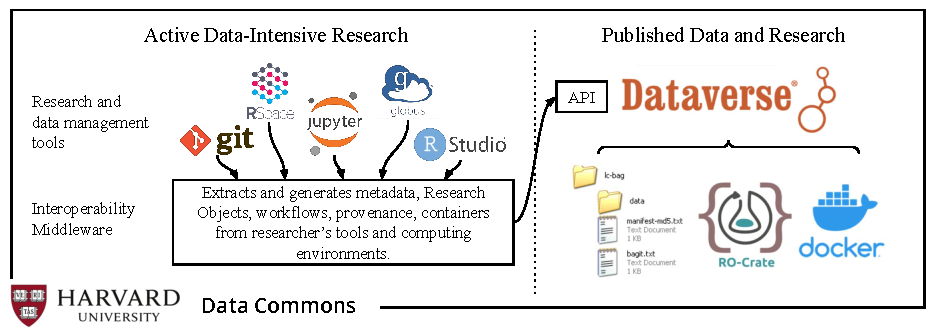
\includegraphics{content/images/data-commons-ro-crate-figure-5.pdf}
\caption{One aspect of Harvard Data Commons. Automatic
encapsulation and deposit of artefacts from data management tools used
during active research at the Harvard Dataverse repository.}
\label{fig:hdc}
\end{figure}

 \section{Related work}% {#relatedwork}

\label{sec:relatedwork}

With the increasing digitisation of research processes, there has been
a significant call for the wider adoption of interoperable sharing of
data and its associated metadata. We refer to
\cite{doi:10.1016/j.patter.2020.100136} for a comprehensive overview and
recommendations, in particular for data; notably that review highlights
the wide variety of metadata and documentation that the literature
prescribes for enabling data reuse. Likewise, we suggest
\cite{doi:10.1016/j.patter.2021.100322} that covers the importance of
metadata standards in reproducible computational research.

Here we focus on approaches for bundling research artefacts along with
their metadata. This notion of publishing compound objects for
scholarly communication has a long history behind it
\cite{doi:10.1190/1.1822162,vandesompel_2007}, but recent approaches
have followed three main strands: (1) publishing to centralised
repositories; (2) packaging approaches similar to RO-Crate; and (3)
bundling the computational workflow around a scientific experiment.

 \subsection{Bundling and packaging digital research artefacts}

Early work making the case for publishing compound scholarly
communication units \cite{vandesompel_2007} led to the development of the
Object Re-Use and Exchange
model\footnote{\url{http://www.openarchives.org/ore/1.0/primer}} (OAI-ORE), providing
a structured \textbf{resource map} of the digital artefacts that together
support a scholarly output.

The challenge of describing computational workflows was one of the main
motivations for the early proposal of \textit{Research Objects} (RO)
\cite{doi:10.1016/j.future.2011.08.004} as first-class citizens for sharing
and publishing. The RO approach involves bundling datasets, workflows,
scripts and results along with traditional dissemination materials like
journal articles and presentations, forming a single package.
Crucially, these resources are not just gathered, but also individually
typed, described and related to each other using semantic vocabularies.
As pointed out in \cite{doi:10.1016/j.future.2011.08.004} an open-ended
\textit{Linked Data} approach is not sufficient for scholarly communication: a
common data model is also needed in addition to common and best
practices for managing and annotating lifecycle, ownership, versioning
and attributions.

Considering the FAIR principles \cite{doi:10.1038/sdata.2016.18}, we can
say with hindsight that the initial RO approaches strongly targeted
\textit{Interoperability}, with a particular focus on the reproducibility of
\textit{in-silico experiments} involving computational workflows and the reuse
of existing RDF vocabularies.

The first implementation of Research Objects for sharing workflows in
myExperiment \cite{doi:10.1093/nar/gkq429} was based on RDF ontologies
\cite{newman2009}, building on Dublin Core, FOAF, SIOC, Creative Commons
and OAI-ORE to form myExperiment ontologies for describing social
networking, attribution and credit, annotations, aggregation packs,
experiments, view statistics, contributions, and workflow components
\cite{myExperimentOntology2009}.

This initially workflow-centric approach was further formalised as the
Wf4Ever Research Object Model \cite{doi:10.1016/j.websem.2015.01.003},
which is a general-purpose research artefact description framework.
This model is based on existing ontologies (FOAF, Dublin Core Terms,
OAI-ORE and AO/OAC precursors to the W3C Web Annotation Model
\cite{Ciccarese:17:WAD}) and adds specializations for workflow models and
executions using W3C PROV-O \cite{PROVO}. The Research Object statements
are saved in a \textit{manifest} (the OAI-ORE \textit{resource map}), with additional
annotation resources containing user-provided details such as title and
description.

We now claim that one barrier for wider adoption of the Wf4Eer Research
Object model for general packaging digital research artefacts was
exactly this re-use of multiple existing vocabularies (FAIR principle
I2: \textit{Metadata use vocabularies that follow FAIR principles}), which in
itself is recognised as a challenge \cite{doi:10.3233/978-1-61499-660-6-9}.
Adapters of the Wf4Ever RO model would have to navigate documentation
of multiple overlapping ontologies, in addition to facing the usual
Semantic Web development choices for RDF serialization formats,
identifier minting and publishing resources on the Web.

Several developments for Research Objects improved on this situation,
such as ROHub used by Earth Sciences
\cite{doi:10.1016/j.future.2019.03.046}, which provides a 
user-interface for making Research Objects, along with Research Object
Bundle \cite{doi:10.5281/zenodo.12586} (RO Bundle), which is a ZIP-archive
embedding data files and a JSON-LD serialization of the manifest with
mappings for a limited set of terms. RO Bundle was also used for
storing detailed workflow run provenance (TavernaPROV
\cite{doi:10.5281/zenodo.51314}).

RO-Bundle evolved to Research Object BagIt
archives,\footnote{\url{https://w3id.org/ro/bagit}} a variant of RO Bundle as a BagIt
archive \cite{doi:10.17487/rfc8493}, used by Big Data Bags
\cite{doi:10.1109/BigData.2016.7840618}, CWLProv
\cite{doi:10.1093/gigascience/giz095} and WholeTale
\cite{doi:10.3233/APC200107,doi:10.1109/eScience.2019.00068}.

\subsection{FAIR Digital Objects}

FAIR Digital Objects (FDO) \cite{doi:10.3390/publications8020021} have been
proposed as a conceptual framework for making digital resources
available in a Digital Objects (DO) architecture which encourages
active use of the objects and their metadata. In particular, an FDO has
five parts: (i) The FDO \textit{content}, bit sequences stored in an
accessible repository; (ii) a \textit{Persistent Identifier} (PID) such as a
DOI that identifies the FDO and can resolve these same parts; (iii)
Associated rich \textit{metadata}, as separate FDOs; (iv) Type definitions,
also separate FDOs; (v) Associated \textit{operations} for the given types. A
Digital Object typed as a Collection aggregates other DOs by reference.

The Digital Object Interface Protocol \cite{doip2.0} can be considered an
``abstract protocol'' of requirements, DOs could be implemented in
multiple ways. One suggested implementation is the FAIR Digital Object
Framework,\footnote{\url{https://fairdigitalobjectframework.org/}} based on HTTP and
the Linked Data Principles. While there is agreement on using PIDs
based on DOIs, consensus on how to represent common metadata, core
types and collections as FDOs has not yet been reached. We argue that
RO-Crate can play an important role for FDOs:
\begin{enumerate}
\item[1.] By providing a predictable and extensible serialisation of
structured metadata.
\item[2.] By formalising how to aggregate digital objects as collections (and
adding their context).
\item[3.] By providing a natural Metadata FDO in the form of the RO-Crate
Metadata File.
\item[4.] By being based on Linked Data and the Schema.org vocabulary, meaning
that PIDs already exist for common types and properties.
\end{enumerate}

At the same time, it is clear that the goal of FDO is broader than that
of RO-Crate; namely, FDOs are active objects with distributed
operations, and add further constraints such as PIDs for every element.
These features improve FAIR features of digital objects and are also
useful for RO-Crate, but they also severely restrict the infrastructure
that needs to be implemented and maintained in order for FDOs to remain
accessible. RO-Crate, on the other hand, is more flexible: it can
minimally be used within any file system structure, or ideally exposed
through a range of Web-based scenarios. A \textit{FAIR profile of RO-Crate}
(e.g. enforcing PID usage) will fit well within a FAIR Digital Object ecosystem.

 \subsection{Packaging workflows}

The use of computational workflows, typically combining a chain of
tools in an analytical pipeline, has gained prominence in particular in
the life sciences. Workflows might be used primarily to improve
computational scalability, as well as to assist in making computed
data results FAIR \cite{doi:10.1162/dint_a_00033}, for instance by
improving reproducibility \cite{doi:10.1016/j.future.2017.01.012}, but also
because programmatic data usage help propagate their metadata and
provenance \cite{doi:10.1002/cpe.1228}. At the same time, workflows raise
additional FAIR challenges, since they can be considered important
research artefacts themselves. This viewpoint poses the problem of
capturing and explaining the computational methods of a pipeline in
sufficient machine-readable detail \cite{doi:10.3233/DS-190026}.

Even when researchers follow current best practices for workflow
reproducibility \cite{doi:10.1016/j.cels.2018.03.014,doi:10.1016/j.future.2017.01.012}, the communication of computational
outcomes through traditional academic publishing routes effectively
adds barriers as authors are forced to rely on a textual manuscript
representations. This hinder reproducibility and FAIR use of the
knowledge previously captured in the workflow.

As a real-life example, let us look at a metagenomics article
\cite{doi:10.1038/s41586-019-0965-1} that describes a computational
pipeline. Here the authors have gone to extraordinary efforts to
document the individual tools that have been reused, including their
citations, versions, settings, parameters and combinations. The
\textit{Methods} section is two pages in tight double-columns with twenty four
additional references, supported by the availability of data on an FTP
server (60 GB) \cite{ebi_ftp_umgs2019} and of open source code in GitHub
Finn-Lab/MGS-gut\footnote{\url{https://github.com/Finn-Lab/MGS-gut}}
\cite{finn-lab-mgsgut}, including the pipeline as shell scripts and
associated analysis scripts in R and Python.

This attention to reporting detail for computational workflows is
unfortunately not yet the norm, and although bioinformatics journals
have strong \textit{data availability} requirements, they frequently do not
require authors to include or cite \textit{software, scripts and pipelines}
used for analysing and producing results \cite{soilandreyes_tweet_2020}.
Indeed, in the absence of a specific requirement and an editorial
policy to back it up -- such as eliminating the reference limit --
authors are effectively discouraged from properly and comprehensively
citing software \cite{doi:10.1038/s41592-019-0350-x}.

However detailed this additional information might be, another
researcher who wants to reuse a particular computational method may
first want to assess if the described tool or workflow is Re-runnable
(executable at all), Repeatable (same results for original inputs on
same platform), Reproducible (same results for original inputs with
different platform or newer tools) and ultimately Reusable (similar
results for different input data), Repurposable (reusing parts of the
method for making a new method) or Replicable (rewriting the workflow
following the method description)
\cite{doi:10.3389/fninf.2017.00069,goble_presentation_2016}.

Following the textual description alone, researchers would be forced to
jump straight to evaluate ``Replicable'' by rewriting the pipeline from
scratch. This can be expensive and error-prone. They would firstly need
to install all the software dependencies and download reference
datasets. This can be a daunting task, which may have to be repeated
multiple times as workflows typically are developed at small scale on
desktop computers, scaled up to local clusters, and potentially put
into production using cloud instances, each of which will have
different requirements for software installations.

In recent years the situation has been greatly improved by software
packaging and container technologies like Docker and Conda, these
technologies have been increasingly adopted in life sciences
\cite{doi:10.1007/s41019-017-0050-4} thanks to collaborative efforts such
as BioConda \cite{doi:10.1038/s41592-018-0046-7} and BioContainers
\cite{doi:10.1093/bioinformatics/btx192}, and support by Linux
distributions (e.g. Debian Med \cite{doi:10.1186/1471-2105-11-S12-S5}). As
of November 2021, more than 9,000 software packages are available in
BioConda alone,\footnote{\url{https://anaconda.org/bioconda/}} and 10,000 containers
in BioContainers.\footnote{\url{https://biocontainers.pro/\#/registry}}

Docker and Conda have been integrated into workflow systems such as
Snakemake \cite{doi:10.1093/bioinformatics/bts480}, Galaxy
\cite{doi:10.1093/nar/gky379} and Nextflow \cite{doi:10.1038/nbt.3820}, meaning
a downloaded workflow definition can now be executed on a ``blank''
machine (except for the workflow engine) with the underlying analytical
tools installed on demand. Even with using containers there is a
reproducibility challenge, for instance Docker Hub's retention policy
will expire container images after six
months,\footnote{\url{https://www.docker.com/blog/docker-hub-image-retention-policy-delayed-and-subscription-updates/}}
or a lack of recording versions of transitive dependencies of Conda
packages could cause incompatibilities if the packages are subsequently updated.

These container and package systems only capture small amounts of
metadata.\footnote{Docker and Conda can use \textit{build recipes}, a set of commands
that construct the container image through downloading and installing
its requirements. However these recipes are effectively another piece
of software code, which may itself decay and become difficult to rerun.} In particular, they do not capture any of the semantic
relationships between their content. Understanding these relationships
is made harder by the opaque wrapping of arbitrary tools with unclear
functionality, licenses and attributions.

From this we see that computational workflows are themselves complex
digital objects that need to be recorded not just as files, but in the
context of their execution environment, dependencies and analytical
purpose in research -- as well as other metadata (e.g. version,
license, attribution and identifiers).

It is important to note that having all these computational details in
order to represent them in an RO-Crate is an ideal scenario -- in
practice there will always be gaps of knowledge, and exposing all
provenance details automatically would require improvements to the data
sources, workflow, workflow engine and its dependencies. RO-Crate can
be seen as a flexible annotation mechanism for augmenting automatic
workflow provenance. Additional metadata can be added manually, e.g.
for sensitive clinical data that cannot be publicly exposed\footnote{FAIR principle A2: \textit{Metadata are accessible, even when the
data are no longer available} \cite{doi:10.1038/sdata.2016.18}.}, or
to cite software that lack persistent identifiers. This inline
\textit{FAIRifying} allows researchers to achieve ``just enough FAIR'' to
explain their computational experiments.

\section{Conclusion}

\label{sec:conclusion}

RO-Crate has been established as an approach to packaging digital
research artefacts with structured metadata. This approach assists
developers and researchers to produce and consume FAIR archives of
their research.

RO-Crate is formed by a set of best practice recommendations, developed
by an open and broad community. These guidelines show how to use ``just
enough'' standards in a consistent way. The use of
structured metadata with a rich base vocabulary can cover
general-purpose contextual relations, with a Linked Data foundation
that ensures extensibility to domain- and application-specific uses. We
can therefore consider an RO-Crate not just as a structured data
archive, but as a multimodal scholarly knowledge graph that can help
``FAIRify'' and combine metadata of existing resources.

The adoption of simple Web technologies in the RO-Crate specification
has helped a rapid development of a wide variety of supporting open
source tools and libraries. RO-Crate fits into the larger landscape of
open scholarly communication and FAIR Digital Object infrastructure,
and can be integrated into data repository platforms. RO-Crate can be
applied as a data/metadata exchange mechanism, assist in long-term
archival preservation of metadata and data, or simply used at a small
scale by individual researchers. Thanks to its strong community
support, new and improved profiles and tools are being continuously
added to the RO-Crate landscape, making it easier for adopters
to find examples and support for their own use case.

\subsection{Strictness vs flexibility}

There is always a tradeoff between flexibility and strictness
\cite{doi:10.1007/s11042-009-0397-2} when deciding on semantics of metadata
models. Strict requirements make it easier for users and code to
consume and populate a model, by reducing choices and having mandated
``slots'' to fill in. But such rigidity can also restrict richness and
applicability of the model, as it in turn enforce the initial
assumptions about what can be described.

RO-Crate attempts to strike a balance between these tensions, and
provides a common metadata framework that encourages extensions.
However, just like the RO-Crate specification can be thought of as a
\textit{core profile} of Schema.org in JSON-LD, we cannot stress the
importance of also establishing domain-specific RO-Crate profiles and
conventions, as explored in Sections~\ref{sec:profiles} and \ref
{sec:inuse}. Specialization comes hand-in-hand with the principle of
\textit{graceful degradation}; RO-Crate applications and users are free to
choose the semantic detail level they participate at, as long as they
follow the common syntactic requirements.

 \section{Future work}% {#futurework}

\label{sec:futurework}

The direction of future RO-Crate work is determined by the community
around it as a collaborative effort. We currently plan on further
outreach, building training material (including a comprehensive
entry-level tutorial) and maturing the reference implementation
libraries. We will also collect and build examples of RO-Crate
\textit{consumption}, e.g. Jupyter Notebooks that query multiple crates using
knowledge graphs. In addition, we are exploring ways to support some
entity types requested by users, e.g. detailed workflow runs or
container provenance, which do not have a good match in Schema.org.
Such support could be added, for instance, by integrating other
vocabularies or by having separated (but linked) metadata files.

Furthermore, we want to better understand how the community uses
RO-Crate in practice and how it contrasts with other related efforts;
this will help us to improve our specification and tools. By
discovering commonalities in emerging usage (e.g. additional Schema.org
types), the community helps to reduce divergence that could otherwise
occur with proliferation of further RO-Crate profiles. We plan to
gather feedback via user studies, with the Linked Open Data community
or as part of EOSC Bring-your-own-Data training events.

We operate in an open community where future and potential users of
RO-Crate are actively welcomed to participate and contribute feedback
and requirements. In addition, we are targeting a wider audience through
extensive outreach
activities\footnote{\url{https://www.researchobject.org/ro-crate/outreach.html}} and
by initiating new connections. Recent contacts include American
Geophysical Union (AGU) on Data Citation Reliquary
\cite{doi:10.5281/zenodo.4916734}, National Institute of Standards and
Technology (NIST) on material science, and
InvenioRDM\footnote{\url{https://inveniosoftware.org/products/rdm/}} used by the
Zenodo data repository. New Horizon Europe projects adapting RO-Crate
include BY-COVID,\footnote{\url{https://by-covid.org/}} which aims to improve FAIR
access to data on COVID-19 and other infectious diseases.

The main addition in the upcoming 1.2 release of the RO-Crate
specifications will be the formalization of
profiles\footnote{\url{https://www.researchobject.org/ro-crate/1.2-DRAFT/profiles}}
for different categories of crates. Additional entity types have been
requested by users, e.g. workflow runs, business workflows, containers
and software packages, tabular data structures; these are not always
matched well with existing Schema.org types, but may benefit from other
vocabularies or even separate metadata files, e.g. from Frictionless
Data.\footnote{\url{https://frictionlessdata.io/}} We will be further aligning
and collaborating with related research artefact description efforts
like CodeMeta\footnote{\url{https://codemeta.github.io/}} for software metadata,
Science-on-Schema.org\footnote{\url{https://science-on-schema.org/}}
\cite{doi:10.5281/zenodo.4477164} for datasets, FAIR Digital
Objects\footnote{\url{https://fairdo.org/}} \cite{doi:10.3390/publications8020021} and
activities in EOSC task forces\footnote{\url{https://www.eosc.eu/task-force-faq}}
including the EOSC Interoperability Framework \cite{doi:10.2777/620649}.




%%%%%%%%%%%%%%%%%%%%%%%%%%%%%%%%%%%%%%%%%%%%%%%%%%%%%%%%%%%%%%%%%%%%%%%%%%
%%%%%%%%%% Supplementary data
%\begin{esm}%[title=]
%\esmtitle{Supplementary data}
%\esmdescription{} is available at: \url{http://dx.doi.org/???}.
%\esmfiletype{pdf} %file type list:
%%http://www.freeformatter.com/mime-types-list.html#mime-types-list
%\esmfilename{MANUSCRIPTsupp.pdf}
%\end{esm}


%% Put support info here:
%\begin{ack}
%\end{ack}
\begin{acks}
This work has received funding from the European Commission's Horizon
2020 research and innovation programme for projects
BioExcel-2\footnote{\url{https://cordis.europa.eu/project/id/823830}}
(H2020-INFRAEDI-2018-1 823830), IBISBA
1.0\footnote{\url{https://cordis.europa.eu/project/id/730976}}
(H2020-INFRAIA-2017-1-two-stage 730976),
PREP-IBISBA\footnote{\url{https://cordis.europa.eu/project/id/871118}}
(H2020-INFRADEV-2019-2 871118),
EOSC-Life\footnote{\url{https://cordis.europa.eu/project/id/824087}}
(H2020-INFRAEOSC-2018-2 824087),
SyntheSys+\footnote{\url{https://cordis.europa.eu/project/id/823827}}
(H2020-INFRAIA-2018-1 823827). From the Horizon Europe Framework
Programme this work has received funding for
BY-COVID\footnote{\url{https://cordis.europa.eu/project/id/101046203}}
(HORIZON-INFRA-2021-EMERGENCY-01 101046203).

Bj\"{o}rn Gr\"{u}ning is supported by DataPLANT (NFDI 7/1 --
42077441\footnote{\url{https://gepris.dfg.de/gepris/projekt/442077441}}), part of the
German National Research Data Infrastructure (NFDI), funded by the
Deutsche Forschungsgemeinschaft (DFG).

Ana Trisovic is funded by the Alfred P. Sloan Foundation (grant number
P-2020-13988).\footnote{\url{https://sloan.org/grant-detail/9555}} Harvard Data
Commons is supported by an award from Harvard University Information
Technology (HUIT).
\end{acks}

 \section*{Contributions}

Author contributions to this article and the RO-Crate project according
to the Contributor Roles Taxonomy CASRAI
CrEDiT\footnote{\url{https://casrai.org/credit/}} \cite{doi:10.1087/20150211}:
\begin{description}
\item[Stian Soiland-Reyes]  Conceptualization, Data curation, Formal Analysis, Funding
acquisition, Investigation, Methodology, Project administration,
Software, Visualization, Writing -- original draft, Writing -- review
\& editing

\item[Peter Sefton]  Conceptualization, Investigation, Methodology, Project
administration, Resources, Software, Writing -- review \& editing

\item[Merc\`{e} Crosas]  Writing -- review \& editing

\item[Leyla Jael Castro]  Methodology, Writing -- review \& editing

\item[Frederik Coppens]  Writing -- review \& editing

\item[Jos\'{e} M. Fern\'{a}ndez]  Methodology, Software, Writing -- review \& editing

\item[Daniel Garijo]  Methodology, Writing -- review \& editing

\item[Bj\"{o}rn Gr\"{u}ning]  Writing -- review \& editing

\item[Marco La Rosa]  Software, Methodology, Writing -- review \& editing

\item[Simone Leo]  Software, Methodology, Writing -- review \& editing

\item[Eoghan \'{O} Carrag\'{a}in]  Investigation, Methodology, Project administration, Writing -- review
\& editing

\item[Marc Portier]  Methodology, Writing -- review \& editing

\item[Ana Trisovic]  Software, Writing -- review \& editing

\item[RO-Crate Community]  Investigation, Software, Validation, Writing -- review \& editing

\item[Paul Groth]  Methodology, Supervision, Writing -- original draft, Writing --
review \& editing

\item[Carole Goble]  Conceptualization, Funding acquisition, Methodology, Project
administration, Supervision, Visualization, Writing -- review \& editing
\end{description}

We would also like to acknowledge contributions from:
\begin{description}
\item[Finn Bacall]
 Software, Methodology

\item[Herbert Van de Sompel]
 Writing -- review \& editing

\item[Ignacio Eguinoa]
 Software, Methodology

\item[Nick Juty]
 Writing -- review \& editing

\item[Oscar Corcho]
 Writing -- review \& editing

\item[Stuart Owen]
 Writing -- review \& editing

\item[Laura Rodr\'iguez-Navas]
 Software, Visualization, Writing -- review \& editing

\item[Alan R. Williams]
 Writing -- review \& editing
\end{description}
\begin{appendix}


\section{Formalizing RO-Crate in First Order Logic}
\label{sec:formaldefinition}

Below is a formalization of the concept of RO-Crate as a set of
relations using First Order Logic.

\subsection{Language}

Definition of language $\mathcal{L}_{\mathit{rocrate}}$:
%
\begin{eqnarray*}
\mathcal{L}_{\mathit{rocrate}} &=& \bigl\{\mathit{Property}(p), \mathit{Class}(c),
\mathit{Value}(x), \mathbb{R}, \mathbb{S} \bigr\}
\\
\mathbb{D} &=& \mathbb{IRI}
\\
\mathbb{IRI} &\equiv& { \text{IRIs as defined in RFC3987 \cite{doi:10.17487/rfc3987}} }
\\
\mathbb{R} &\equiv& { \text{real or integer numbers} }
\\
\mathbb{S} &\equiv& { \text{literal strings} }
\end{eqnarray*}

The domain of discourse $\mathbb{D}$ is the set of $\mathbb{IRI}$
identifiers (notation \texttt
{<http://example.\noxml{\break}com/>}),\footnote{For simplicity, blank nodes are not included in this formalisation, as RO-Crate
recommends the use of IRI identifiers: \url
{https://www.researchobject.org/ro-crate/1.1/appendix/jsonld.html\#describing-entities-in-json-ld}.} with additional descriptions using numbers $\mathbb{R}$ (notation
$13.37$) and literal strings $\mathbb{S}$ (notation $\text{``Hello''}$).

From this formalised language $\mathcal{L}_{\mathit{rocrate}}$ we can interpret
an RO-Crate in any representation that can gather these descriptions,
their properties, classes, and literal attributes.

\subsection{Minimal RO-Crate}

Below we use $\mathcal{L}_{\mathit{rocrate}}$ to define a minimal\footnote{The full
list of types, relations and attribute properties from the
RO-Crate specification are not included. Examples shown include
$\textit{datePublished}$, $\textit{CreativeWork}$ and $\textit{name}$.
} RO-Crate:
%
\begin{eqnarray*}
\textit{ROCrate}(R) & \models& \textit{Root}(R) \land \textit{Mentions}(R, R)
\land \textit{hasPart}(R, d) \land
\\
& & {}\textit{Mentions}(R, d) \land \textit{DataEntity}(d) \land
\\
& & {}\textit{Mentions}(R, c) \land \textit{ContextualEntity}(c)
\\
\forall r \ \textit{Root}(r) & \Rightarrow& \textit{Dataset}(r) \land
\textit{name}(r, n) \land \textit{description}(r, d) \land
\\
& &{} \textit{datePublished}(r, date) \land \textit{license}(e, l)
\\
\forall e \forall n \ \textit{name}(e, n) & \Rightarrow& \textit{Value}(n)
\\
\forall e \forall s \ \textit{description}(e, s) & \Rightarrow&
\textit{Value}(s)
\\
\forall e \forall d \ \textit{datePublished}(e, d) & \Rightarrow&
\textit{Value}(d)
\\
\forall e \forall l \ \textit{license}(e, l) & \Rightarrow&
\textit{ContextualEntity}(l)
\\
\textit{DataEntity}(e) & \equiv& \textit{File}(e) \oplus \textit{Dataset}(e)
\\
\textit{Entity}(e) & \equiv& \textit{DataEntity}(e) \lor \textit{ContextualEntity}(e)
\\
\forall e \ \textit{Entity}(e) & \Rightarrow& \textit{type}(e, c) \land
\textit{Class}(c)
\\
\forall e \ \textit{ContextualEntity}(e) & \Rightarrow& \textit{name}(e, n)
\\
\textit{Mentions}(R, s) & \models& \textit{Relation}(s, p, e) \oplus
\textit{Attribute}(s, p, l)
\\
\textit{Relation}(s, p, o) & \models& \textit{Entity}(s) \land
\textit{Property}(p) \land \textit{Entity}(o)
\\
\textit{Attribute}(s, p, v) & \models& \textit{Entity}(s) \land
\textit{Property}(p) \land \textit{Value}(v)
\\
\textit{Value}(v) & \equiv& v \in\mathbb{R} \oplus v \in\mathbb{S}
\end{eqnarray*}

An $\textit{ROCrate}(R)$ is defined as a self-described \emph{Root Data Entity},
which contains parts (\emph{data entities}), which are
further described in \emph{contextual entities}. These terms align with
their use in the RO-Crate 1.1 terminology.\footnote{\url{https://www.researchobject.org/ro-crate/1.1/terminology}}

The $\textit{Root}(r)$ is a type of $\textit{Dataset}(r)$, and must as metadata 
have at least the attributes $\textit{name}$, $description$ and
$\textit{datePublished}$ as literal values, as well as a contextual entity that identify its
$\textit{license}$. These predicates correspond to the RO-Crate 1.1 minimal requirements
for the root data entity.\footnote{\url
{https://www.researchobject.org/ro-crate/1.1/root-data-entity.html\#direct-properties-of-the-root-data-entity}}

The concept of an $\textit{Entity}(e)$ is introduced as being either a
$\textit{DataEntity}(e)$, a $\textit{ContextualEntity}(e)$, or both.\footnote{\url
{https://www.researchobject.org/ro-crate/1.1/contextual-entities.html\#contextual-vs-data-entities}} Any $\textit{Entity}(e)$ must be
typed with at least one $\textit{Class}(c)$, and
every $\textit{ContextualEntity}(e)$ must also have a $\textit{name}(e,n)$; this
corresponds to expectations for any \emph{referenced contextual entity}
(Section~\ref{sec:contextualentities}).

For simplicity in this formalization (and to assist production rules
below) $R$ is a constant representing a single RO-Crate, typically
written to independent RO-Crate Metadata files. $R$ is used by
$\textit{Mentions}(R, e)$ to indicate that $e$ is an Entity described by the
RO-Crate and therefore its metadata (a set of $\textit{Relation}$ and
$\textit{Attribute}$ predicates) form part of the RO-Crate serialization.
$\textit{Relation}(s, p, o)$ and $\textit{Attribute}(s, p, x)$ are defined as a \emph
{subject--predicate--object} triple pattern from an $\textit{Entity}(s)$ using
a $\textit{Property}(p)$ to either another $\textit{Entity}(o)$ or a $\textit{Value}(x)$ value.

\subsection{Example of formalised RO-Crate}

The below is an example RO-Crate represented using the above
formalisation, assuming a base IRI of \texttt{<http://example.com/ro/123/>}:
%
{\fontsize{9.7}{11.7}\selectfont{\begin{gather*}
\textit{ROCrate}(\texttt{<http://example.com/ro/123/>})
\\
\textit{name}\bigl(\texttt{<http://example.com/ro/123/>},
\\
\quad \text{``Data files associated with the manuscript:Effects of {
\ldots}''}\bigr)
\\
\textit{description}\bigl(\texttt{<http://example.com/ro/123/>},
\\
\quad \text{``Palliative care planning for nursing home residents {
\ldots}''}\bigr)
\\
\textit{license}(\texttt{<http://example.com/ro/123/>},
\\
\quad \texttt{<https://spdx.org/licenses/CC-BY-4.0>})
\\
\textit{datePublished}\bigl(\texttt{<http://example.com/ro/123/>}, \text
{``2017-02-23''}\bigr)
\\
\textit{hasPart}(\texttt{<http://example.com/ro/123/>}, \texttt{<http://example.com/ro/123/file.txt>})
\\
\textit{hasPart}(\texttt{<http://example.com/ro/123/>}, \texttt{<http://example.com/ro/123/interviews/>})
\\
\\
\textit{ContextualEntity}(\texttt{<https://spdx.org/licenses/CC-BY-4.0>})
\\
\textit{name}\bigl(\texttt{<https://spdx.org/licenses/CC-BY-4.0>},
\\
\quad \text{``Creative Commons Attribution 4.0''}\bigr)
\\
\\
\textit{ContextualEntity}(\texttt{<https://spdx.org/licenses/CC-BY-NC-4.0>})
\\
\textit{name}\bigl(\texttt{<https://spdx.org/licenses/CC-BY-NC-4.0>},
\\
\quad \text{``Creative Commons Attribution Non Commercial 4.0''}
\bigr)
\\
\\
\textit{File}(\texttt{<http://example.com/ro/123/survey.csv>})
\\
\textit{name}\bigl(\texttt{<http://example.com/ro/123/survey.csv>},
\text{``Survey of care providers''}\bigr)
\\
\\
\textit{Dataset}(\texttt{<http://example.com/ro/123/interviews/>})
\\
\textit{name}\bigl(\texttt{<http://example.com/ro/123/interviews/>},
\\
\quad \text{``Audio recordings of care provider interviews''}
\bigr)
\\
\textit{license}(\texttt{<http://example.com/ro/123/interviews/>},
\\*
\quad \texttt{<https://spdx.org/licenses/CC-BY-NC-4.0>})
\end{gather*}}}

Notable from this triple-like formalization is that a RO-Crate $R$ is
fully represented as a tree at depth 2 helped by the use of
%PDAG%
$\mathbh{IRI}$
%PDAG%
nodes. For instance the aggregation from the root entity
$\textit{hasPart}(\texttt{{\ldots}interviews/>})$ is at same level as the data
entity's property \textit{license}(\texttt{{\ldots}CC-BY-\noxml{\break}NC-4.0>}) and that
contextual entity's attribute $ \textit{name}(\text{{\ldots}Non Commercial
4.0''})$. As shown in Section~\ref{sec:jsonld}, the RO-Crate Metadata
File serialization is an equivalent shallow tree, although at depth 3
to cater for the JSON-LD preamble of \texttt{"@context"} and \texttt{"@graph"}.

In reality many additional attributes and contextual types from
Schema.org types like \url{http://schema.org/affiliation} and \url
{http://schema.org/Organization} would be used to further describe the
RO-Crate and its entities, but as these are optional (\textit{SHOULD}
requirements) they do not form part of this formalization.

\subsection{Mapping to RDF with Schema.org}

A formalised RO-Crate in $\mathcal{L}_{\mathit{rocrate}}$ can be mapped to
different serializations.
Assume a simplified\footnote{This simplification and mapping does not cover the extensive list of literal
datatypes built into RDF 1.1, only strings and decimal real numbers.
Likewise, \textit{LanguageTag} is deliberately not utillised below.} language $\mathcal{L}_{\textit{RDF}}$
based on the RDF abstract syntax \cite{rdfworkinggroup_2014}:
%
{\fontsize{9.8}{11.8}\selectfont{\begin{eqnarray*}
\mathcal{L}_{\textit{RDF}} & \equiv& \bigl\{ \textit{Triple}(s,p,o),
\textit{IRI}(i), \textit{BlankNode}(b), \textit{Literal}(s), \mathbb{IRI},
\mathbb{S}, \mathbb{R} \bigr\}
\\
\mathbb{D}_{\textit{RDF}} & \equiv& \mathbb{S}
\\
\forall i \ \textit{IRI}(i) & \Rightarrow& i \in\mathbb{IRI}
\\
\forall s \forall p \forall o \ \textit{Triple}(s,p,o) & \Rightarrow& \bigl(
\textit{IRI}(s) \lor \textit{BlankNode}(s) \bigr) \land
\\
& & \textit{IRI}(p) \land
\\
& & \bigl(\textit{IRI}(o) \lor \textit{BlankNode}(o) \lor \textit{Literal}(o)
\bigr)
\\
\textit{Literal}(v) & \models& \textit{Value}(v) \land \textit{Datatype}(v,t)
\land \textit{IRI}(t)
\\
\forall v \ \textit{Value}(v) & \Rightarrow& v \in\mathbb{S}
\\
\textit{LanguageTag}(v, l) & \equiv& Datatype (v,
\\
&& \texttt{<http://www.w3.org/1999/02/22-rdf-syntax-ns\#langString>} )
\end{eqnarray*}}}

Below follows a mapping from $\mathcal{L}_{\mathit{rocrate}}$ to $\mathcal
{L}_{\textit{RDF}}$ using Schema.org as vocabulary:
%
{\fontsize{9.6}{11.6}\selectfont{\begin{eqnarray*}
\textit{Property}(p) & \Rightarrow& \textit{type}(p, \texttt
{<http://www.w3.org/2000/01/rdf-schema\#Property>})
\\
\textit{Class}(c) & \Rightarrow& \textit{type}(c, \texttt {<http://www.w3.org/2000/01/rdf-schema\#Class>})
\\
\textit{Dataset}(d) & \Rightarrow& \textit{type}(d, \texttt {<http://schema.org/Dataset>})
\\
\textit{File}(f) & \Rightarrow& \textit{type}(f, \texttt {<http://schema.org/MediaObject>})
\\
\textit{ContextualEntity}(e) & \Rightarrow& \textit{type}(f, \texttt
{<http://schema.org/Thing>})
\\
\textit{CreativeWork}(e) & \Rightarrow& \textit{ContextualEntity}(e) \land
\textit{type}(e, \texttt{<http://schema.org/CreativeWork>})
\\
\textit{hasPart}(e, t) & \Rightarrow& \textit{Relation}(e, \texttt
{<http://schema.org/hasPart>}, t)
\\
\textit{name}(e, n) & \Rightarrow& \textit{Attribute}(e, \texttt
{<http://schema.org/name>}, n)
\\
\textit{description}(e, s) & \Rightarrow& \textit{Attribute}(e, \texttt
{<http://schema.org/description>}, s)
\\
\textit{datePublished}(e, d) & \Rightarrow& Attribute(e, \texttt
{<http://schema.org/datePublished>}, d)
\\
\textit{license}(e, l) & \Rightarrow& \textit{Relation}(e, \texttt
{<http://schema.org/license>}, l) \land \textit{CreativeWork}(l)
\\
\textit{type}(e, t) & \Rightarrow& \textit{Relation}(e, \texttt
{<http://www.w3.org/1999/02/22-rdf-syntax-ns\#type>}, t)
\\
& & {}\land \textit{Class}(t)
\\
\textit{String}(s) & \equiv& \textit{Value}(s) \land s \in\mathbb{S}
\\
\textit{String}(s) & \Rightarrow& \textit{Datatype}(s, \texttt
{<http://www.w3.org/2001/XMLSchema\#string>})
\\
\textit{Decimal}(d) & \equiv& \textit{Value}(d) \land d \in\mathbb{R}
\\
\textit{Decimal}(d) & \Rightarrow& \textit{Datatype}(d, \texttt
{<http://www.w3.org/2001/XMLSchema\#decimal>})
\\
\textit{Relation}(s,p,o) & \Rightarrow& \textit{Triple}(s,p,o) \land
\textit{IRI}(s) \land \textit{IRI}(o)
\\
\textit{Attribute}(s,p,o) & \Rightarrow& \textit{Triple}(s,p,o) \land
\textit{IRI}(s) \land \textit{Literal}(o)
\end{eqnarray*}}}

Note that in the JSON-LD serialization of RO-Crate, the expression of
$\textit{Class}$ and $\textit{Property}$ is typically indirect: The JSON-LD \texttt
{@context} maps to Schema.org IRIs, which, when resolved as Linked
Data, embed their formal definition as RDFa. Extensions may however
include such term definitions directly in the RO-Crate.

\subsection{RO-Crate 1.1 Metadata File Descriptor}

An important RO-Crate principle is that of being \textbf
{self-described}. Therefore the serialisation of the RO-Crate into a
file should also describe itself in a Metadata File Descriptor,\footnote{\url
{https://www.researchobject.org/ro-crate/1.1/root-data-entity.html\#ro-crate-metadata-file-descriptor}} indicating it is $\textit{about}$ (describing) the RO-Crate root data entity,
and that it $\textit{conformsTo}$ a particular version of the RO-Crate specification:
%
\begin{eqnarray*}
\textit{about}(s,o) & \Rightarrow& \textit{Relation}(s, \texttt
{<http://schema.org/about>}, o)
\\
\textit{conformsTo}(s,o) & \Rightarrow& \textit{Relation}(s, \texttt
{<http://purl.org/dc/terms/conformsTo>}, o)
\\
\textit{MetadataFile}(m) & \Rightarrow& \textit{CreativeWork}(m) \land
\textit{about}(m,R) \land \textit{ROCrate}(R) \land
\\
& &{} \textit{conformsTo}(m, \texttt{<https://w3id.org/ro/crate/1.1>})
\end{eqnarray*}

Note that although the metadata file necessarily is an \emph
{information resource} written to disk or served over the network (as
JSON-LD), it is not considered to be a contained \emph{part} of the
RO-Crate in the form of a \emph{data entity}, rather it is described
only as a \emph{contextual entity}.

In the conceptual model, the \emph{RO-Crate Metadata File} can be seen
as the top-level node that describes the \emph{RO-Crate Root}, however
in the formal model (and the JSON-LD format) the metadata file
descriptor is an additional contextual entity that is not affecting the
depth-limit of the RO-Crate.

\subsection{Forward-chained production rules for JSON-LD}

Combining the above predicates and Schema.org mapping with rudimentary
JSON templates, these forward-chaining production rules can output
JSON-LD according to the RO-Crate 1.1 specification:\footnote{\textbf{Limitations:}
 Contextual entities not related from the
RO-Crate (e.g. using inverse relations to a data entity) would not be
covered by the single direction $Mentions(R, s)$ production rule; see
\href{https://github.com/ResearchObject/ro-crate/issues/122}{GitHub
issue ResearchObject/ro-crate\#122}. The $\textit{datePublished}(e, d)$ rule do
not include syntax checks for the ISO 8601 datetime format. Compared
with RO-Crate examples, this generated JSON-LD does not use a
$\textit{@context}$ as the IRIs are produced unshortened, a post-step could do
JSON-LD Flattening with a versioned RO-Crate context. The \texttt
{@type} expansion is included for clarity, even though this is also
implied by the $\textit{type}(e, t)$ expansion to $\textit{Relation}(e, \texttt{xsd:type})$.}
%
\begin{eqnarray*}
\textit{Mentions}(R, s) \land \textit{Relation}(s,p,o) & \Rightarrow&
\textit{Mentions}(R, o)
\\
\textit{IRI}(i) & \Rightarrow& \texttt{"} i \texttt{"}
\\
\textit{Decimal}(d) & \Rightarrow& d
\\
\textit{String}(s) & \Rightarrow& \texttt{"} s \texttt{"}
\\
\forall e \forall t \ \textit{type}(e, t) & \Rightarrow& \texttt{\{"@id":} e
\texttt{,}
\\
&& \ \ \texttt{"@type":} t
\\
&& \texttt{\}}
\\
\forall s \forall p \forall o \ \textit{Relation}(s,p,o) & \Rightarrow& 
\texttt{\{"@id":} s \texttt{,}
\\
&& \ \ p \texttt{: \{"@id":} o \texttt{\}}
\\
&& \texttt{\}}
\\
\forall s \forall p \forall v \ \textit{Attribute}(s,p,v) & \Rightarrow&
\texttt{\{"@id":} s \texttt{,}
\\
&& \ \ p \texttt{:} v
\\
&& \texttt{\}}
\\
\forall r \forall c\ \textit{ROCrate}(r) & \Rightarrow& 
\texttt{\{"@graph": [}
\\
&& \ \ \ \ \ \ \textit{Mentions}(r, c)*
\\
&& \ \ \ \texttt{]}
\\
&& \texttt{\}}
\\
R & \equiv& \texttt{<./>}
\\
R & \Rightarrow& \textit{MetadataFile}(\texttt{<ro-crate-metadata.json>})
\end{eqnarray*}

This exposes the first order logic domain of discourse of IRIs, with
rational numbers and strings as their corresponding JSON-LD
representation. These production rules first grow the graph of $R$ by
adding a transitive rule -- anything described in $R$ which is related
to $o$, means that $o$ is also mentioned by the $\textit{ROCrate}(R)$. For
simplicity this rule is one-way; in theory the graph can also contain
free-standing contextual entities that have outgoing relations to data-
and contextual entities, but these are proposed to be bound to the root
data entity with Schema.org relation \url{http://schema.org/mentions}.


\section{RO-Crate Community}

\label{sec:communitylist}

As of 2021-10-04, the \textit{RO-Crate} Community members are:
\begin{itemize}
\item[*] Peter Sefton \url{https://orcid.org/0000-0002-3545-944X} (co-chair)
\item[*] Stian Soiland-Reyes \url{https://orcid.org/0000-0001-9842-9718} (co-chair)
\item[*] Eoghan \'{O} Carrag\'{a}in \url
{https://orcid.org/0000-0001-8131-2150} (emeritus chair)
\item[*] Oscar Corcho \url{https://orcid.org/0000-0002-9260-0753}
\item[*] Daniel Garijo \url{https://orcid.org/0000-0003-0454-7145}
\item[*] Raul Palma \url{https://orcid.org/0000-0003-4289-4922}
\item[*] Frederik Coppens \url{https://orcid.org/0000-0001-6565-5145}
\item[*] Carole Goble \url{https://orcid.org/0000-0003-1219-2137}
\item[*] Jos\'{e} Mar\'ia Fern\'{a}ndez \url{https://orcid.org/0000-0002-4806-5140}
\item[*] Kyle Chard \url{https://orcid.org/0000-0002-7370-4805}
\item[*] Jose Manuel Gomez-Perez \url{https://orcid.org/0000-0002-5491-6431}
\item[*] Michael R Crusoe \url{https://orcid.org/0000-0002-2961-9670}
\item[*] Ignacio Eguinoa \url{https://orcid.org/0000-0002-6190-122X}
\item[*] Nick Juty \url{https://orcid.org/0000-0002-2036-8350}
\item[*] Kristi Holmes \url{https://orcid.org/0000-0001-8420-5254}
\item[*] Jason A. Clark \url{https://orcid.org/0000-0002-3588-6257}
\item[*] Salvador Capella-Gutierrez \url{https://orcid.org/0000-0002-0309-604X}
\item[*] Alasdair J. G. Gray \url{https://orcid.org/0000-0002-5711-4872}
\item[*] Stuart Owen \url{https://orcid.org/0000-0003-2130-0865}
\item[*] Alan R Williams \url{https://orcid.org/0000-0003-3156-2105}
\item[*] Giacomo Tartari \url{https://orcid.org/0000-0003-1130-2154}
\item[*] Finn Bacall \url{https://orcid.org/0000-0002-0048-3300}
\item[*] Thomas Thelen \url{https://orcid.org/0000-0002-1756-2128}
\item[*] Herv\'{e} M\'{e}nager \url{https://orcid.org/0000-0002-7552-1009}
\item[*] Laura Rodr\'iguez-Navas \url{https://orcid.org/0000-0003-4929-1219}
\item[*] Paul Walk \url{https://orcid.org/0000-0003-1541-5631}
\item[*] brandon whitehead \url{https://orcid.org/0000-0002-0337-8610}
\item[*] Mark Wilkinson \url{https://orcid.org/0000-0001-6960-357X}
\item[*] Paul Groth \url{https://orcid.org/0000-0003-0183-6910}
\item[*] Erich Bremer \url{https://orcid.org/0000-0003-0223-1059}
\item[*] LJ Garcia Castro \url{https://orcid.org/0000-0003-3986-0510}
\item[*] Karl Sebby \url{https://orcid.org/0000-0001-6022-9825}
\item[*] Alexander Kanitz \url{https://orcid.org/0000-0002-3468-0652}
\item[*] Ana Trisovic \url{https://orcid.org/0000-0003-1991-0533}
\item[*] Gavin Kennedy \url{https://orcid.org/0000-0003-3910-0474}
\item[*] Mark Graves \url{https://orcid.org/0000-0003-3486-8193}
\item[*] Jasper Koehorst \url{https://orcid.org/0000-0001-8172-8981}
\item[*] Simone Leo \url{https://orcid.org/0000-0001-8271-5429}
\item[*] Marc Portier \url{https://orcid.org/0000-0002-9648-6484}
\item[*] Paul Brack \url{https://orcid.org/0000-0002-5432-2748}
\item[*] Milan Ojster\v{s}ek \url{https://orcid.org/0000-0003-1743-8300}
\item[*] Bert Droesbeke \url{https://orcid.org/0000-0003-0522-5674}
\item[*] Chenxu Niu \url{https://github.com/UstcChenxu}
\item[*] Kosuke Tanabe \url{https://orcid.org/0000-0002-9986-7223}
\item[*] Tomasz Miksa \url{https://orcid.org/0000-0002-4929-7875}
\item[*] Marco La Rosa \url{https://orcid.org/0000-0001-5383-6993}
\item[*] Cedric Decruw \url{https://orcid.org/0000-0001-6387-5988}
\item[*] Andreas Czerniak \url{https://orcid.org/0000-0003-3883-4169}
\item[*] Jeremy Jay \url{https://orcid.org/0000-0002-5761-7533}
\item[*] Sergio Serra \url{https://orcid.org/0000-0002-0792-8157}
\item[*] Ronald Siebes \url{https://orcid.org/0000-0001-8772-7904}
\item[*] Shaun de Witt \url{https://orcid.org/0000-0003-4196-3658}
\item[*] Shady El Damaty \url{https://orcid.org/0000-0002-2318-4477}
\item[*] Douglas Lowe \url{https://orcid.org/0000-0002-1248-3594}
\item[*] Sergio Serra \url{https://orcid.org/0000-0002-0792-8157}
\item[*] Xuanqi Li \url{https://orcid.org/0000-0003-1498-6205}
\end{itemize}
\end{appendix}



%\markdownInput{../content/70.acknowledgements.md}

%%%% Appendix

%\newpage
%\appendix
%%\markdownInput{../content/80.formal-definition.md}
%% Because this file is added with \include, do not use
% Markdown setions within.
%
% Edit here before syncing to 80.formal-definition.md for HTML version


\section{Formalizing RO-Crate in First Order Logic}

\label{sec:formaldefinition}

Below is a formalization of the concept of RO-Crate as a set of relations using First Order Logic:

\subsection{Language}

Definition of language $\mathcal{L}_{rocrate}$:

\begin{eqnarray*}
    \mathcal{L}_{rocrate}   & = & \big\{ Property(p), Class(c),
                            Value(x), \mathbb{R}, \mathbb{S} \big\} \\
    \mathbb{D}              & = & \mathbb{IRI} \\
    \mathbb{IRI}            & \equiv & { \text{IRIs as defined in RFC3987} } \\
    \mathbb{R}              & \equiv & { \text{real or integer numbers} } \\
    \mathbb{S}              & \equiv & { \text{literal strings} }
\end{eqnarray*}


The domain of discourse $\mathbb{D}$ is the set of $\mathbb{IRI}$ identifiers \cite{doi:10.17487/rfc3987} (notation $\texttt{<http://example.com/>}$)\footnote{
    For simplicity, blank nodes are not included in this formalisation, as RO-Crate
    recommends the use of IRI identifiers: \url{https://www.researchobject.org/ro-crate/1.1/appendix/jsonld.html\#describing-entities-in-json-ld}
}, with additional descriptions using numbers $\mathbb{R}$ (notation $13.37$) and literal strings $\mathbb{S}$ (notation $\text{“Hello”}$).

From this formalised language $\mathcal{L}_{rocrate}$ we can interpret an RO-Crate in any representation that can gather these descriptions, their properties, classes, and literal attributes.

\subsection{Minimal RO-Crate}

Below we use $\mathcal{L}_{rocrate}$ to define a minimal\footnote{
    The full list of types, relations and attribute properties from the RO-Crate specification are not included. Examples shown include $datePublished$, $CreativeWork$ and $name$.
} RO-Crate:


\begin{eqnarray*}
ROCrate(R)                                  & \models & Root(R) \land Mentions(R, R) \land hasPart(R, d) \land \\
                                            & & Mentions(R, d) \land DataEntity(d) \land \\
                                            & & Mentions(R, c) \land ContextualEntity(c) \\
\forall r \ Root(r)                         & \Rightarrow & Dataset(r) \land name(r, n) \land description(r, d) \land \\
                                            & &             datePublished(r, date) \land license(e, l) \\
\forall e \forall n \ name(e, n)            & \Rightarrow & Value(n) \\
\forall e \forall s \ description(e, s)     & \Rightarrow & Value(s) \\
\forall e \forall d \ datePublished(e, d)   & \Rightarrow & Value(d) \\
\forall e \forall l \ license(e, l)         & \Rightarrow & ContextualEntity(l) \\
DataEntity(e)                               & \equiv &      File(e) \oplus Dataset(e) \\
Entity(e)                                   & \equiv &      DataEntity(e) \lor ContextualEntity(e) \\
\forall e \ Entity(e)                       & \Rightarrow & type(e, c) \land Class(c) \\
\forall e \ ContextualEntity(e)             & \Rightarrow & name(e, n)  \\
Mentions(R, s)                              & \models &     Relation(s, p, e) \oplus Attribute(s,  p, l) \\
Relation(s, p, o)                           & \models &     Entity(s) \land Property(p) \land  Entity(o) \\
Attribute(s, p, v)                          & \models &     Entity(s) \land Property(p) \land Value(v) \\
Value(v)                                    & \equiv &      v \in \mathbb{R} \oplus v \in \mathbb{S}
\end{eqnarray*}

An $ROCrate(R)$ is defined as a self-described \emph{Root Data Entity}, which describes and contains parts (\emph{data entities}), which are further described in \emph{contextual entities}.  These terms align with their use in the RO-Crate 1.1 terminology\footnote{
    \url{https://www.researchobject.org/ro-crate/1.1/terminology}}.

The $Root(r)$ is a type of $Dataset(r)$, and must have the metadata to literal attributes to provide a $name$, $description$ and $datePublished$, as well as a contextual entity identifying its license. These predicates correspond to the RO-Crate 1.1 requirements for the root data entity\footnote{
    \url{https://www.researchobject.org/ro-crate/1.1/root-data-entity.html\#direct-properties-of-the-root-data-entity}
}.

The concept of an $Entity(e)$ is introduced as being either a $DataEntity(e)$, a $ContextualEntity(e)$, or both\footnote{
    \url{https://www.researchobject.org/ro-crate/1.1/contextual-entities.html\#contextual-vs-data-entities}
}. Any $Entity(e)$ must be typed with at least one $Class(c)$, and every $ContextualEntity(e)$ must also have a $name(e,n)$; this corresponds to expectations for any \emph{referenced contextual entity} (section \ref{sec:contextualentities}). 

For simplicity in this formalization (and to assist production rules below) $R$ is a constant representing a single RO-Crate, typically written to independent RO-Crate Metadata files. $R$ is used by $Mentions(R, e)$ to indicate that $e$ is an Entity described by the RO-Crate and therefore its metadata (a set of $Relation$ and $Attribute$ predicates) form part of the RO-Crate serialization. $Relation(s, p, o)$ and $Attribute(s, p, x)$ are defined as a \emph{subject—predicate—object} triple pattern from an $Entity(s)$ using a $Property(p)$ to either another $Entity(o)$ or a $Value(x)$ value.

\subsection{Example of formalized RO-Crate}

The below is an example RO-Crate represented using the above formalisation, assuming a base URI of \texttt{<http://example.com/ro/123/>}:

\allowdisplaybreaks
\begin{eqnarray*}
&& ROCrate(\texttt{<http://example.com/ro/123/>}) \\
&& name(\texttt{<http://example.com/ro/123/>}, \\
&& \ \ \ \ \ \text{“Data files associated with the manuscript:Effects of …”}) \\
&& description(\texttt{<http://example.com/ro/123/}, \\
&& \ \ \ \ \ \text{“Palliative care planning for nursing home residents …”}) \\
&& license(\texttt{<http://example.com/ro/123/>}, \\
&& \ \ \ \ \ \texttt{<https://spdx.org/licenses/CC-BY-4.0>}) \\
&& datePublished(\texttt{<http://example.com/ro/123/>}, \text{“2017-02-23”}) \\
&& hasPart(\texttt{<http://example.com/ro/123/>},
        \texttt{<http://example.com/ro/123/file.txt>}) \\
&& hasPart(\texttt{<http://example.com/ro/123/>},
        \texttt{<http://example.com/ro/123/interviews/>}) \\
\\
&& ContextualEntity(\texttt{<https://spdx.org/licenses/CC-BY-4.0>}) \\
&& name(\texttt{<https://spdx.org/licenses/CC-BY-4.0>},  \\
&& \ \ \ \ \  \text{Creative Commons Attribution 4.0”}) \\
\\
&& ContextualEntity(\texttt{<https://spdx.org/licenses/CC-BY-NC-4.0>}) \\
&& name(\texttt{<https://spdx.org/licenses/CC-BY-NC-4.0>},  \\
&& \ \ \ \ \  \text{Creative Commons Attribution Non Commercial 4.0”}) \\
\\
&& File(\texttt{<http://example.com/ro/123/survey.csv>}) \\
&& name(\texttt{<http://example.com/ro/123/survey.csv>},
        \text{“Survey of care providers”}) \\
\\
&& Dataset(\texttt{<http://example.com/ro/123/interviews/>}) \\
&& name(\texttt{<http://example.com/ro/123/interviews/>},  \\
&& \ \ \ \ \  \text{“Audio recordings of care provider interviews”}) \\
&& license(\texttt{<http://example.com/ro/123/interviews/>}, \\
&& \ \ \ \ \ \texttt{<https://spdx.org/licenses/CC-BY-NC-4.0>})
\end{eqnarray*}


Notable from this triple-like formalization is that a RO-Crate $R$ is fully represented as a tree at depth 2 helped by the use of $𝕀𝕣𝕚$ nodes. For instance the aggregation from the root entity $hasPart(\texttt{…interviews/>})$ is at same level as the data entity’s property $license(\texttt{…CC-BY-NC-4.0>})$ and that contextual entity’s attribute $ name(\text{…Non Commercial 4.0”})$. As shown in section \ref{sec:jsonld}, the RO-Crate Metadata File serialization is an equivalent shallow tree, although at depth 3 to cater for the JSON-LD preamble of \texttt{"@context"} and \texttt{"@graph"}.

In reality many additional attributes and contextual types from Schema.org types like \url{http://schema.org/affiliation} and \url{http://schema.org/Organization} would be used to further describe the RO-Crate and its entities, but as these are optional (\textit{SHOULD} requirements) they do not form part of this formalization.


\subsection{Mapping to RDF with Schema.org}

A formalized RO-Crate in $\mathcal{L}_{rocrate}$ can be mapped to different serializations.
Assume a simplified\footnote{
 This simplification does not cover the extensive list of literal datatypes built-in to RDF 1.1, only strings and decimal real numbers. Likewise, language of literals are not included.
} language $\mathcal{L}_{RDF}$
based on the RDF abstract syntax \cite{rdfworkinggroup_2014}:

\begin{eqnarray*}
\mathcal{L}_{RDF}           & \equiv &      \big\{ Triple(s,p,o), IRI(i), BlankNode(b), Literal(s),
    \mathbb{IRI}, \mathbb{S}, \mathbb{R}    \big\} \\
\mathbb{D}_{RDF}            & \equiv &      \mathbb{S} \\
\forall i \ IRI(i)          & \Rightarrow & i \in \mathbb{IRI} \\
\forall s \forall p \forall o \
    Triple(s,p,o)           & \Rightarrow & \Big( IRI(s) \lor BlankNode(s) \Big) \land  \\
                            & &             IRI(p) \land  \\
                            & &             \Big(IRI(o) \lor BlankNode(o) \lor Literal(o) \Big) \\
Literal(v)                  & \models &     Value(v) \land Datatype(v,t) \land IRI(t) \\
\forall v \ Value(v)        & \Rightarrow & v \in \mathbb{S} \\
LanguageTag(v, l)           & \equiv &      Datatype\big(v, \\
    && \texttt{<http://www.w3.org/1999/02/22-rdf-syntax-ns\#langString>}\big)
\end{eqnarray*}

Below follows a mapping from $\mathcal{L}_{rocrate}$ to $\mathcal{L}_{RDF}$ using Schema.org as vocabulary:

\begin{eqnarray*}
Property(p)         & \Rightarrow &     type(p, \texttt{<http://www.w3.org/2000/01/rdf-schema\#Property>})   \\
Class(c)            & \Rightarrow &     type(c, \texttt{<http://www.w3.org/2000/01/rdf-schema\#Class>})  \\
Dataset(d)          & \Rightarrow &     type(d, \texttt{<http://schema.org/Dataset>})   \\
File(f)             & \Rightarrow &     type(f, \texttt{<http://schema.org/MediaObject>})   \\
ContextualEntity(e) & \Rightarrow &     type(f, \texttt{<http://schema.org/Thing>})   \\
CreativeWork(e)     & \Rightarrow &     ContextualEntity(e) \land type(e, \texttt{<http://schema.org/CreativeWork>})  \\
hasPart(e, t)       & \Rightarrow &     Relation(e, \texttt{<http://schema.org/hasPart>}, t)    \\
name(e, n)          & \Rightarrow &     Attribute(e, \texttt{<http://schema.org/name>}, n)  \\
description(e, s)   & \Rightarrow &     Attribute(e, \texttt{<http://schema.org/description>}, s)   \\
datePublished(e, d) & \Rightarrow &     Attribute(e, \texttt{<http://schema.org/datePublished>}, d) \\
license(e, l)       & \Rightarrow &     Relation(e, \texttt{<http://schema.org/license>}, l) \land CreativeWork(l) \\
type(e, t)          & \Rightarrow &     Relation(e, \texttt{<http://www.w3.org/1999/02/22-rdf-syntax-ns\#type>}, t) \\
                    & & \land Class(t)   \\
String(s)           & \equiv &          Value(s) \land  s \in \mathbb{S} \\
String(s)           & \Rightarrow &     Datatype(s, \texttt{<http://www.w3.org/2001/XMLSchema\#string>}) \\
Decimal(d)          & \equiv &          Value(d) \land  d \in \mathbb{R} \\
Decimal(d)          & \Rightarrow &     Datatype(d, \texttt{<http://www.w3.org/2001/XMLSchema\#decimal>}) \\
Relation(s,p,o)     & \Rightarrow &     Triple(s,p,o) \land IRI(s) \land IRI(o) \\
Attribute(s,p,o)    & \Rightarrow &     Triple(s,p,o) \land IRI(s) \land Literal(o) \\
\end{eqnarray*}

Note that in the JSON-LD serialization of RO-Crate, the expression of $Class$ and $Property$ is typically indirect: The JSON-LD \texttt{@context} maps to Schema.org IRIs, which, when resolved as Linked Data, embed their formal definition as RDFa. Extensions may however include such term definitions directly in the RO-Crate.

\subsection{RO-Crate 1.1 Metadata File Descriptor}

An important RO-Crate principle is that of being \textbf{self-described} Therefore the serialisation of the RO-Crate into a file should also describe itself in a Metadata File Descriptor\footnote{
    \url{https://www.researchobject.org/ro-crate/1.1/root-data-entity.html\#ro-crate-metadata-file-descriptor}
}, indicating it is $about$ (describing) the RO-Crate root data entity, and that it $conformsTo$ a particular version of the RO-Crate specification:

\begin{eqnarray*}
about(s,o)      & \Rightarrow & Relation(s, \texttt{<http://schema.org/about>}, o)   \\
conformsTo(s,o) & \Rightarrow & Relation(s, \texttt{<http://purl.org/dc/terms/conformsTo>}, o)   \\
MetadataFile(m) & \Rightarrow & CreativeWork(m) \land about(m,R) ∧ ROCrate(R) \land    \\
                &             & conformsTo(m, \texttt{<https://w3id.org/ro/crate/1.1>})
\end{eqnarray*}

Note that although the metadata file necessarily is an \emph{information resource} written to disk or served over the network (as JSON-LD), it is not considered to be a contained \emph{part} of the RO-Crate in the form of a \emph{data entity}, rather it is described only as a \emph{contextual entity}.

In the conceptual model the \emph{RO-Crate Metadata File} can be seen as the top-level node that describes the \emph{RO-Crate Root}, however in the formal model (and the JSON-LD format) the metadata file descriptor is an additional contextual entity that is not affecting the depth-limit of the RO-Crate.

\subsection{Forward-chained Production Rules for JSON-LD}

Combining the above predicates and Schema.org mapping with rudimentary JSON templates, these forward-chaining production rules can output JSON-LD according to the RO-Crate 1.1 specification\footnote{
    \textbf{Limitations:} Contextual entities not related from the RO-Crate (e.g. using inverse relations to a data entity) would not be covered by the single direction $Mentions(R, s)$ production rule; see \href{https://github.com/ResearchObject/ro-crate/issues/122}{GitHub issue ResearchObject/ro-crate\#122}. The $datePublished(e, d)$ rule do not include syntax checks for the ISO 8601 datetime format. Compared with RO-Crate examples, this generated JSON-LD does not use a $@context$ as the IRIs are produced unshortened, a post-step could do JSON-LD Flattening with a versioned RO-Crate context. The \texttt{@type} expansion is included for clarity, even though this is also implied by the $type(e, t)$ expansion to $Relation(e, \texttt{xsd:type})$.
}:

\begin{eqnarray*}
Mentions(R, s) \land Relation(s,p,o)
                        & \Rightarrow & Mentions(R, o) \\
IRI(i)                  & \Rightarrow & \texttt{"} i \texttt{"} \\
Decimal(d)              & \Rightarrow & d \\
String(s)               & \Rightarrow & \texttt{"} s \texttt{"} \\
\forall e \forall t
\ type(e, t)            & \Rightarrow & \texttt{\{"@id":}  e \texttt{,} \\
&&                               \ \  \texttt{"@type":} t \\
&&                              \texttt{\}} \\
\forall s \forall p \forall o
\ Relation(s,p,o)
                        & \Rightarrow &  \texttt{\{"@id":}  s \texttt{,} \\
&&                               \ \  p \texttt{: \{ "@id":} o \texttt{\}} \\
&&                              \texttt{\}} \\
\forall s \forall p \forall v
\ Attribute(s,p,v)    & \Rightarrow &  \texttt{\{"@id":} s \texttt{,} \\
&&                               \ \ p \texttt{:} v  \\
&&                               \texttt{\}} \\
\forall r  \forall c
    ROCrate(r)      & \Rightarrow &  \texttt{\{ "@graph": [} \\
&& \ \ \ \ Mentions(r, c)* \\
&& \ \ \ \texttt{]} \\
&& \texttt{\}} \\
R   & \equiv & \texttt{<./>}  \\
R   & \Rightarrow &  MetadataFile(\texttt{<ro-crate-metadata.json>}) \\
\end{eqnarray*}

This exposes the first order logic domain of discourse of IRIs, with rational numbers and strings as their corresponding JSON-LD representation. These production rules first grow the graph of $R$ by adding a transitive rule – anything described in $R$ which is related to $o$, means that $o$ is also mentioned by the $ROCrate(R)$. For simplicity this rule is one-way; in theory the graph can also contain free-standing contextual entities that have outgoing relations to data- and contextual entities, but these are proposed to be bound to the root data entity with Schema.org relation \href{http://schema.org/mentions}.


%\newpage
%\markdownInput{../content/89.community.md}

%%%%%%%%%%% The bibliography starts:
%\nocite{label}
%\bibliographystyle{ios1}
%\bibliography{ro-crate}

% Explicit bibliography from proof
%
% structpyb loaded by imikolaityte, 2021-12-28 10:21:28
%
\begin{thebibliography}{}

%%% bbsrt2.pl, ver. 2.5.8, 2017.08.09
%b1 ###bbsrt2
%b122 ###
\bibitem{doi:10.1093/nar/gky379}
%
\begin{barticle}
\bauthor{\binits{E.}~\bsnm{Afgan}},
\bauthor{\binits{D.}~\bsnm{Baker}},
\bauthor{\binits{B.}~\bsnm{Batut}},
\bauthor{\binits{M.}~\bsnm{van den Beek}},
\bauthor{\binits{D.}~\bsnm{Bouvier}},
\bauthor{\binits{M.}~\bsnm{Cech}},
\bauthor{\binits{J.}~\bsnm{Chilton}},
\bauthor{\binits{D.}~\bsnm{Clements}},
\bauthor{\binits{N.}~\bsnm{Coraor}},
\bauthor{\binits{B.A.}~\bsnm{Gr\"{u}ning}},
\bauthor{\binits{A.}~\bsnm{Guerler}},
\bauthor{\binits{J.}~\bsnm{Hillman-Jackson}},
\bauthor{\binits{S.}~\bsnm{Hiltemann}},
\bauthor{\binits{V.}~\bsnm{Jalili}},
\bauthor{\binits{H.}~\bsnm{Rasche}},
\bauthor{\binits{N.}~\bsnm{Soranzo}},
\bauthor{\binits{J.}~\bsnm{Goecks}},
\bauthor{\binits{J.}~\bsnm{Taylor}},
\bauthor{\binits{A.}~\bsnm{Nekrutenko}} and
\bauthor{\binits{D.}~\bsnm{Blankenberg}},
\batitle{The Galaxy platform for accessible, reproducible and collaborative
biomedical analyses: 2018 update},
\bjtitle{Nucleic Acids Research}
\bvolume{46}(\bissue{W1})
(\byear{2018}),
\bfpage{W537}--\blpage{W544}.
\bid{doi={10.1093/nar/gky379}}
\end{barticle}
%
\OrigBibText
E.~Afgan,
D.~Baker,
B.~Batut,
M.~van~den Beek,
D.~Bouvier,
M.~Cech,
J.~Chilton,
D.~Clements,
N.~Coraor,
B.A.~Gr\"{u}ning,
A.~Guerler,
J.~Hillman-Jackson,
S.~Hiltemann,
V.~Jalili,
H.~Rasche,
N.~Soranzo,
J.~Goecks,
J.~Taylor,
A.~Nekrutenko and
D.~Blankenberg,
\textit{The Galaxy platform for accessible, reproducible and collaborative
biomedical analyses: 2018 update.},
Nucleic Acids Research
46(W1)
(2018),
W537--W544.
doi:10.1093/nar/gky379.
\endOrigBibText
\bptok{structpyb}
\endbibitem

%b2 ###bbsrt2
%b124 ###
\bibitem{doi:10.5281/zenodo.4916734}
%
\begin{botherref}
\oauthor{\binits{D.}~\bsnm{Agarwal}},
\oauthor{\binits{C.}~\bsnm{Goble}},
\oauthor{\binits{S.}~\bsnm{Soiland-Reyes}},
\oauthor{\binits{U.}~\bsnm{Sarkans}},
\oauthor{\binits{D.}~\bsnm{Noesgaard}},
\oauthor{\binits{U.}~\bsnm{Schindler}},
\oauthor{\binits{M.}~\bsnm{Fenner}},
\oauthor{\binits{P.}~\bsnm{Manghi}},
\oauthor{\binits{S.}~\bsnm{Stall}},
\oauthor{\binits{C.}~\bsnm{Coward}} and
\oauthor{\binits{C.}~\bsnm{Erdmann}},
Data Citation Community of Practice -- 8,
Workshop, Zenodo/AGU, 2021.
\url{https://data.agu.org/DataCitationCoP/2nd-workshop-data-citation}.
\bid{doi={10.5281/zenodo.4916734}}
\end{botherref}
%
\OrigBibText
D.~Agarwal,
C.~Goble,
S.~Soiland-Reyes,
U.~Sarkans,
D.~Noesgaard,
U.~Schindler,
M.~Fenner,
P.~Manghi,
S.~Stall,
C.~Coward and
C.~Erdmann,
Data Citation Community of Practice -- 8 June 2021 Workshop,
Zenodo/AGU,
2021.
doi:10.5281/zenodo.4916734.
\url{https://data.agu.org/DataCitationCoP/2nd-workshop-data-citation}.
\endOrigBibText
\bptok{structpyb}
\endbibitem

%b3 ###bbsrt2
%b87 ###
\bibitem{dcat2}
%
\begin{botherref}
\oauthor{\binits{R.}~\bsnm{Albertoni}},
\oauthor{\binits{D.}~\bsnm{Browning}},
\oauthor{\binits{S.}~\bsnm{Cox}},
\oauthor{\binits{A.}~\bsnm{Gonzalez Beltran}},
\oauthor{\binits{A.}~\bsnm{Perego}},
\oauthor{\binits{P.}~\bsnm{Winstanley}} and
\binstitute{Dataset Exchange Working Group},
Data Catalog Vocabulary
({DCAT}) -- Version 2,
\textit{{W3C} Recommendation}
(2020),
\url{https://www.w3.org/TR/2020/REC-vocab-dcat-2-20200204/}.
\end{botherref}
%
\OrigBibText
R.~Albertoni,
D.~Browning,
S.~Cox,
A.~Gonzalez~Beltran,
A.~Perego,
P.~Winstanley and
Dataset Exchange Working Group:
Data Catalog Vocabulary ({DCAT}) - Version 2,
{W3C} Recommendation,
2020.
\url{https://www.w3.org/TR/2020/REC-vocab-dcat-2-20200204/}.
\endOrigBibText
\bptok{structpyb}
\endbibitem

%b4 ###bbsrt2
%b111 ###
\bibitem{doi:10.1038/s41586-019-0965-1}
%
\begin{barticle}
\bauthor{\binits{A.}~\bsnm{Almeida}},
\bauthor{\binits{A.L.}~\bsnm{Mitchell}},
\bauthor{\binits{M.}~\bsnm{Boland}},
\bauthor{\binits{S.C.}~\bsnm{Forster}},
\bauthor{\binits{G.B.}~\bsnm{Gloor}},
\bauthor{\binits{A.}~\bsnm{Tarkowska}},
\bauthor{\binits{T.D.}~\bsnm{Lawley}} and
\bauthor{\binits{R.D.}~\bsnm{Finn}},
\batitle{A new genomic blueprint of the human gut microbiota},
\bjtitle{Nature}
\bvolume{568}(\bissue{7753})
(\byear{2019}),
\bfpage{499}--\blpage{504}.
\bid{doi={10.1038/s41586-019-0965-1}}
\end{barticle}
%
\OrigBibText
A.~Almeida,
A.L.~Mitchell,
M.~Boland,
S.C.~Forster,
G.B.~Gloor,
A.~Tarkowska,
T.D.~Lawley and
R.D.~Finn,
\textit{A new genomic blueprint of the human gut microbiota.},
Nature
568(7753)
(2019),
499--504.
doi:10.1038/s41586-019-0965-1.
\endOrigBibText
\bptok{structpyb}
\endbibitem

%b5 ###bbsrt2
%b77 ###
\bibitem{doi:10.1371/journal.pbio.3000099}
%
\begin{barticle}
\bauthor{\binits{G.}~\bsnm{Alterovitz}},
\bauthor{\binits{D.}~\bsnm{Dean}},
\bauthor{\binits{C.}~\bsnm{Goble}},
\bauthor{\binits{M.R.}~\bsnm{Crusoe}},
\bauthor{\binits{S.}~\bsnm{Soiland-Reyes}},
\bauthor{\binits{A.}~\bsnm{Bell}},
\bauthor{\binits{A.}~\bsnm{Hayes}},
\bauthor{\binits{A.}~\bsnm{Suresh}},
\bauthor{\binits{A.}~\bsnm{Purkayastha}},
\bauthor{\binits{C.H.}~\bsnm{King}},
\bauthor{\binits{D.}~\bsnm{Taylor}},
\bauthor{\binits{E.}~\bsnm{Johanson}},
\bauthor{\binits{E.E.}~\bsnm{Thompson}},
\bauthor{\binits{E.}~\bsnm{Donaldson}},
\bauthor{\binits{H.}~\bsnm{Morizono}},
\bauthor{\binits{H.}~\bsnm{Tsang}},
\bauthor{\binits{J.K.}~\bsnm{Vora}},
\bauthor{\binits{J.}~\bsnm{Goecks}},
\bauthor{\binits{J.}~\bsnm{Yao}},
\bauthor{\binits{J.S.}~\bsnm{Almeida}},
\bauthor{\binits{J.}~\bsnm{Keeney}},
\bauthor{\binits{K.}~\bsnm{Addepalli}},
\bauthor{\binits{K.}~\bsnm{Krampis}},
\bauthor{\binits{K.M.}~\bsnm{Smith}},
\bauthor{\binits{L.}~\bsnm{Guo}},
\bauthor{\binits{M.}~\bsnm{Walderhaug}},
\bauthor{\binits{M.}~\bsnm{Schito}},
\bauthor{\binits{M.}~\bsnm{Ezewudo}},
\bauthor{\binits{N.}~\bsnm{Guimera}},
\bauthor{\binits{P.}~\bsnm{Walsh}},
\bauthor{\binits{R.}~\bsnm{Kahsay}},
\bauthor{\binits{S.}~\bsnm{Gottipati}},
\bauthor{\binits{T.C.}~\bsnm{Rodwell}},
\bauthor{\binits{T.}~\bsnm{Bloom}},
\bauthor{\binits{Y.}~\bsnm{Lai}},
\bauthor{\binits{V.}~\bsnm{Simonyan}} and
\bauthor{\binits{R.}~\bsnm{Mazumder}},
\batitle{Enabling precision medicine via standard communication of {HTS}
provenance, analysis, and results},
\bjtitle{PLOS Biology}
\bvolume{16}(\bissue{12})
(\byear{2018}),
\bnumber{e3000099}.
\bid{doi={10.1371/journal.pbio.3000099}}
\end{barticle}
%
\OrigBibText
G.~Alterovitz,
D.~Dean,
C.~Goble,
M.R.~Crusoe,
S.~Soiland-Reyes,
A.~Bell,
A.~Hayes,
A.~Suresh,
A.~Purkayastha,
C.H.~King,
D.~Taylor,
E.~Johanson,
E.E.~Thompson,
E.~Donaldson,
H.~Morizono,
H.~Tsang,
J.K.~Vora,
J.~Goecks,
J.~Yao,
J.S.~Almeida,
J.~Keeney,
K.~Addepalli,
K.~Krampis,
K.M.~Smith,
L.~Guo,
M.~Walderhaug,
M.~Schito,
M.~Ezewudo,
N.~Guimera,
P.~Walsh,
R.~Kahsay,
S.~Gottipati,
T.C.~Rodwell,
T.~Bloom,
Y.~Lai,
V.~Simonyan and
R.~Mazumder,
\textit{Enabling precision medicine via standard communication of {HTS}
provenance, analysis, and results.},
{PLOS} Biology
16(12)
(2018),
e3000099.
doi:10.1371/journal.pbio.3000099.
\endOrigBibText
\bptok{structpyb}
\endbibitem

%b6 ###bbsrt2
%b14 ###
\bibitem{doi:10.1007/s10209-016-0475-y}
%
\begin{barticle}
\bauthor{\binits{R.C.}~\bsnm{Amorim}},
\bauthor{\binits{J.A.}~\bsnm{Castro}},
\bauthor{\binits{J.}~\bsnm{Rocha da Silva}} and
\bauthor{\binits{C.}~\bsnm{Ribeiro}},
\batitle{A comparison of research data management platforms: Architecture,
flexible metadata and interoperability},
\bjtitle{Universal Access in the Information Society}
(\byear{2016}),
\bfpage{1}--\blpage{12}.
\bid{doi={10.1007/s10209-016-0475-y}}
\end{barticle}
%
\OrigBibText
R.C.~Amorim,
J.A.~Castro,
J.~Rocha~da Silva and
C.~Ribeiro,
A comparison of research data management platforms: architecture, flexible
metadata and interoperability,
\textit{Universal Access in the Information Society}
\textbf{00}
(2016),
1--12.
doi:10.1007/s10209-016-0475-y.
\endOrigBibText
\bptok{structpyb}
\endbibitem

%b7 ###bbsrt2
%b56 ###
\bibitem{doi:10.5281/zenodo.3922136}
%
\begin{bbook}
\bauthor{\binits{G.}~\bsnm{Arfaoui}} and
\bauthor{\binits{M.}~\bsnm{Jaoua}},
\bbtitle{{RO}-Crate {RDA} {maDMP} Mapper, Zenodo},
\byear{2020}.
\url{https://github.com/GhaithArf/ro-crate-rda-madmp-mapper}.
\bid{doi={10.5281/zenodo.3922136}}
\end{bbook}
%
\OrigBibText
G.~Arfaoui and
M.~Jaoua,
\textit{{RO}-Crate {RDA} {maDMP} Mapper},
Zenodo
(2020).
doi:10.5281/zenodo.3922136.
\url{https://github.com/GhaithArf/ro-crate-rda-madmp-mapper}.
\endOrigBibText
\bptok{structpyb}
\endbibitem

%b8 ###bbsrt2
%b55 ###
\bibitem{ro-composer}
%
\begin{botherref}
\oauthor{\binits{F.}~\bsnm{Bacall}},
\oauthor{\binits{S.}~\bsnm{Soiland-Reyes}} and
\oauthor{\binits{M.}~\bsnm{Soares e Silva}},
eScienceLab: RO-Composer. \url
{https://esciencelab.org.uk/projects/ro-composer/}.
\end{botherref}
%
\OrigBibText
F.~Bacall,
S.~Soiland-Reyes and
M.~Soares~e Silva,
eScienceLab: RO-Composer.
\url{https://esciencelab.org.uk/projects/ro-composer/}.
\endOrigBibText
\bptok{structpyb}
\endbibitem

%b9 ###bbsrt2
%b46 ###
\bibitem{ro-crate-ruby}
%
\begin{botherref}
\oauthor{\binits{F.}~\bsnm{Bacall}} and
\oauthor{\binits{M.}~\bsnm{Whitwell}},
{GitHub} -- {ResearchObject}/ro-crate-ruby: A Ruby gem for creating,
manipulating and reading {RO}-Crates.
\url{https://github.com/ResearchObject/ro-crate-ruby}.
\end{botherref}
%
\OrigBibText
F.~Bacall and
M.~Whitwell,
{GitHub} - {ResearchObject}/ro-crate-ruby: A Ruby gem for creating,
manipulating and reading {RO}-Crates.
\url{https://github.com/ResearchObject/ro-crate-ruby}.
\endOrigBibText
\bptok{structpyb}
\endbibitem

%b10 ###bbsrt2
%b64 ###
\bibitem{doi:10.1371/journal.ppat.1008643}
%
\begin{barticle}
\bauthor{\binits{D.}~\bsnm{Baker}},
\bauthor{\binits{M.}~\bsnm{van den Beek}},
\bauthor{\binits{D.}~\bsnm{Blankenberg}},
\bauthor{\binits{D.}~\bsnm{Bouvier}},
\bauthor{\binits{J.}~\bsnm{Chilton}},
\bauthor{\binits{N.}~\bsnm{Coraor}},
\bauthor{\binits{F.}~\bsnm{Coppens}},
\bauthor{\binits{I.}~\bsnm{Eguinoa}},
\bauthor{\binits{S.}~\bsnm{Gladman}},
\bauthor{\binits{B.}~\bsnm{Gr\"{u}ning}},
\bauthor{\binits{N.}~\bsnm{Keener}},
\bauthor{\binits{D.}~\bsnm{Larivi\`{e}re}},
\bauthor{\binits{A.}~\bsnm{Lonie}},
\bauthor{\binits{S.}~\bsnm{Kosakovsky Pond}},
\bauthor{\binits{W.}~\bsnm{Maier}},
\bauthor{\binits{A.}~\bsnm{Nekrutenko}},
\bauthor{\binits{J.}~\bsnm{Taylor}} and
\bauthor{\binits{S.}~\bsnm{Weaver}},
\batitle{No more business as usual: Agile and effective responses to emerging
pathogen threats require open data and open analytics},
\bjtitle{PLOS Pathogens}
\bvolume{16}(\bissue{8})
(\byear{2020}),
\bnumber{e1008643}.
\bid{doi={10.1371/journal.ppat.1008643}}
\end{barticle}
%
\OrigBibText
D.~Baker,
M.~van~den Beek,
D.~Blankenberg,
D.~Bouvier,
J.~Chilton,
N.~Coraor,
F.~Coppens,
I.~Eguinoa,
S.~Gladman,
B.~Gr\"{u}ning,
N.~Keener,
D.~Larivi\`{e}re,
A.~Lonie,
S.~Kosakovsky~Pond,
W.~Maier,
A.~Nekrutenko,
J.~Taylor and
S.~Weaver,
\textit{No more business as usual: Agile and effective responses to emerging
pathogen threats require open data and open analytics.},
{PLOS} Pathogens
16(8)
(2020),
e1008643.
doi:10.1371/journal.ppat.1008643.
\endOrigBibText
\bptok{structpyb}
\endbibitem

%b11 ###bbsrt2
%b89 ###
\bibitem{doi:10.5334/dsj-2019-044}
%
\begin{barticle}
\bauthor{\binits{M.}~\bsnm{Barker}},
\bauthor{\binits{R.}~\bsnm{Wilkinson}} and
\bauthor{\binits{A.}~\bsnm{Treloar}},
\batitle{The Australian Research Data Commons},
\bjtitle{Data Science Journal}
\bvolume{18}
(\byear{2019}).
\bid{doi={10.5334/dsj-2019-044}}
\end{barticle}
%
\OrigBibText
M.~Barker,
R.~Wilkinson and
A.~Treloar,
The Australian Research Data Commons,
\textit{Data Science Journal}
\textbf{18}
(2019), 00.
doi:10.5334/dsj-2019-044.
\endOrigBibText
\bptok{structpyb}
\endbibitem

%b12 ###bbsrt2
%b11 ###
\bibitem{doi:10.1016/j.future.2011.08.004}
%
\begin{barticle}
\bauthor{\binits{S.}~\bsnm{Bechhofer}},
\bauthor{\binits{I.}~\bsnm{Buchan}},
\bauthor{\binits{D.}~\bsnm{De Roure}},
\bauthor{\binits{P.}~\bsnm{Missier}},
\bauthor{\binits{J.}~\bsnm{Ainsworth}},
\bauthor{\binits{J.}~\bsnm{Bhagat}},
\bauthor{\binits{P.}~\bsnm{Couch}},
\bauthor{\binits{D.}~\bsnm{Cruickshank}},
\bauthor{\binits{M.}~\bsnm{Delderfield}},
\bauthor{\binits{I.}~\bsnm{Dunlop}},
\bauthor{\binits{M.}~\bsnm{Gamble}},
\bauthor{\binits{D.}~\bsnm{Michaelides}},
\bauthor{\binits{S.}~\bsnm{Owen}},
\bauthor{\binits{D.}~\bsnm{Newman}},
\bauthor{\binits{S.}~\bsnm{Sufi}} and
\bauthor{\binits{C.}~\bsnm{Goble}},
\batitle{Why linked data is not enough for scientists},
\bjtitle{Future Generation Computer Systems}
\bvolume{29}(\bissue{2})
(\byear{2013}),
\bfpage{599}--\blpage{611}.
\bid{doi={10.1016/j.future.2011.08.004}}
\end{barticle}
%
\OrigBibText
S.~Bechhofer,
I.~Buchan,
D.~De~Roure,
P.~Missier,
J.~Ainsworth,
J.~Bhagat,
P.~Couch,
D.~Cruickshank,
M.~Delderfield,
I.~Dunlop,
M.~Gamble,
D.~Michaelides,
S.~Owen,
D.~Newman,
S.~Sufi and
C.~Goble,
\textit{Why linked data is not enough for scientists},
Future Generation Computer Systems
29(2)
(2013),
599--611.
doi:10.1016/j.future.2011.08.004.
\endOrigBibText
\bptok{structpyb}
\endbibitem

%b13 ###bbsrt2
%b59 ###
\bibitem{CheckMyCrate}
%
\begin{botherref}
\oauthor{\binits{K.}~\bsnm{Belchev}},
{KockataEPich}/{CheckMyCrate}: A command line application for
validating a {RO}-Crate object against a {JSON} profile,
\textit{GitHub}
(2021).
\url{https://github.com/KockataEPich/CheckMyCrate}.
\end{botherref}
%
\OrigBibText
K.~Belchev,
{KockataEPich}/{CheckMyCrate}: A command line application for
validating a
{RO}-Crate object against a {JSON} profile.,
GitHub,
2021.
\url{https://github.com/KockataEPich/CheckMyCrate}.
\endOrigBibText
\bptok{structpyb}
\endbibitem

%b14 ###bbsrt2
%b12 ###
\bibitem{doi:10.1016/j.websem.2015.01.003}
%
\begin{barticle}
\bauthor{\binits{K.}~\bsnm{Belhajjame}},
\bauthor{\binits{J.}~\bsnm{Zhao}},
\bauthor{\binits{D.}~\bsnm{Garijo}},
\bauthor{\binits{M.}~\bsnm{Gamble}},
\bauthor{\binits{K.}~\bsnm{Hettne}},
\bauthor{\binits{R.}~\bsnm{Palma}},
\bauthor{\binits{E.}~\bsnm{Mina}},
\bauthor{\binits{O.}~\bsnm{Corcho}},
\bauthor{\binits{J.M.}~\bsnm{G\'{o}mez-P\'{e}rez}},
\bauthor{\binits{S.}~\bsnm{Bechhofer}},
\bauthor{\binits{G.}~\bsnm{Klyne}} and
\bauthor{\binits{C.}~\bsnm{Goble}},
\batitle{Using a suite of ontologies for preserving workflow-centric
research objects},
\bjtitle{Web Semantics: Science, Services and Agents on the World Wide Web}
\bvolume{32}
(\byear{2015}),
\bfpage{16}--\blpage{42}.
\bid{doi={10.1016/j.websem.2015.01.003}}
\end{barticle}
%
\OrigBibText
K.~Belhajjame,
J.~Zhao,
D.~Garijo,
M.~Gamble,
K.~Hettne,
R.~Palma,
E.~Mina,
O.~Corcho,
J.M.~G\'{o}mez-P\'{e}rez,
S.~Bechhofer,
G.~Klyne and
C.~Goble,
\textit{Using a suite of ontologies for preserving workflow-centric research
objects},
Web Semantics: Science, Services and Agents on the World Wide Web
32
(2015),
16--42.
doi:10.1016/j.websem.2015.01.003.
\endOrigBibText
\bptok{structpyb}
\endbibitem

%b15 ###bbsrt2
%b116 ###
\bibitem{doi:10.3389/fninf.2017.00069}
%
\begin{barticle}
\bauthor{\binits{F.C.Y.}~\bsnm{Benureau}} and
\bauthor{\binits{N.P.}~\bsnm{Rougier}},
\batitle{Re-run, repeat, reproduce, reuse, replicate: Transforming code
into scientific contributions},
\bjtitle{Frontiers in Neuroinformatics}
\bvolume{11}
(\byear{2017}),
\bnumber{69}.
\bid{doi={10.3389/fninf.2017.00069}}
\end{barticle}
%
\OrigBibText
F.C.Y.~Benureau and
N.P.~Rougier,
\textit{Re-run, Repeat, Reproduce, Reuse, Replicate: Transforming Code into
Scientific Contributions.},
Frontiers in Neuroinformatics
11
(2017),
69.
doi:10.3389/fninf.2017.00069.
\endOrigBibText
\bptok{structpyb}
\endbibitem

%b16 ###bbsrt2
%b8 ###
\bibitem{doi:10.1093/nar/gkl971}
%
\begin{barticle}
\bauthor{\binits{H.}~\bsnm{Berman}},
\bauthor{\binits{K.}~\bsnm{Henrick}},
\bauthor{\binits{H.}~\bsnm{Nakamura}} and
\bauthor{\binits{J.L.}~\bsnm{Markley}},
\batitle{The worldwide Protein Data Bank ({wwPDB}): Ensuring a single,
uniform archive of {PDB} data},
\bjtitle{Nucleic Acids Research}
\bvolume{35}\bcomment{(Database issue)}
(\byear{2007}),
\bfpage{D301}--\blpage{D303}.
\bid{doi={10.1093/nar/gkl971}}
\end{barticle}
%
\OrigBibText
H.~Berman,
K.~Henrick,
H.~Nakamura and
J.L.~Markley,
\textit{The worldwide Protein Data Bank ({wwPDB}): ensuring a single, uniform
archive of {PDB} data}.
Nucleic Acids Research
35 (Database issue)
(2007),
D301--3.
doi:10.1093/nar/gkl971.
\endOrigBibText
\bptok{structpyb}
\endbibitem

%b17 ###bbsrt2
%b68 ###
\bibitem{doi:10.5281/zenodo.4705078}
%
\begin{barticle}
\bauthor{\binits{F.}~\bsnm{Bietrix}},
\bauthor{\binits{J.M.}~\bsnm{Carazo}},
\bauthor{\binits{S.}~\bsnm{Capella-Gutierrez}},
\bauthor{\binits{F.}~\bsnm{Coppens}},
\bauthor{\binits{M.L.}~\bsnm{Chiusano}},
\bauthor{\binits{R.}~\bsnm{David}},
\bauthor{\binits{J.M.}~\bsnm{Fernandez}},
\bauthor{\binits{M.}~\bsnm{Fratelli}},
\bauthor{\binits{J.-K.}~\bsnm{Heriche}},
\bauthor{\binits{C.}~\bsnm{Goble}},
\bauthor{\binits{P.}~\bsnm{Gribbon}},
\bauthor{\binits{P.}~\bsnm{Holub}},
\bauthor{\binits{R.P.}~\bsnm{Joosten}},
\bauthor{\binits{S.}~\bsnm{Leo}},
\bauthor{\binits{S.}~\bsnm{Owen}},
\bauthor{\binits{H.}~\bsnm{Parkinson}},
\bauthor{\binits{R.}~\bsnm{Pieruschka}},
\bauthor{\binits{L.}~\bsnm{Pireddu}},
\bauthor{\binits{L.}~\bsnm{Porcu}},
\bauthor{\binits{M.}~\bsnm{Raess}},
\bauthor{\binits{L.}~\bsnm{Rodriguez- Navas}},
\bauthor{\binits{A.}~\bsnm{Scherer}},
\bauthor{\binits{S.}~\bsnm{Soiland-Reyes}} and
\bauthor{\binits{J.}~\bsnm{Tang}},
\batitle{{EOSC}-life methodology framework to enhance reproducibility
within {EOSC}-life},
\bjtitle{Zenodo}
(\byear{2021}).
\bid{doi={10.5281/zenodo.4705078}}
\end{barticle}
%
\OrigBibText
F.~Bietrix,
J.M.~Carazo,
S.~Capella-Gutierrez,
F.~Coppens,
M.L.~Chiusano,
R.~David,
J.M.~Fernandez,
M.~Fratelli,
J.-K.~Heriche,
C.~Goble,
P.~Gribbon,
P.~Holub,
R.~P.~Joosten,
S.~Leo,
S.~Owen,
H.~Parkinson,
R.~Pieruschka,
L.~Pireddu,
L.~Porcu,
M.~Raess,
L.~Rodriguez-~Navas,
A.~Scherer,
S.~Soiland-Reyes and
J.~Tang,
\textit{{EOSC}-Life Methodology framework to enhance reproducibility within
{EOSC}-Life},
Zenodo
(2021).
doi:10.5281/zenodo.4705078.
\endOrigBibText
\bptok{structpyb}
\endbibitem

%b18 ###bbsrt2
%b29 ###
\bibitem{doi:10.4018/978-1-60960-593-3.ch008}
%
\begin{bchapter}
\bauthor{\binits{C.}~\bsnm{Bizer}},
\bauthor{\binits{T.}~\bsnm{Heath}} and
\bauthor{\binits{T.}~\bsnm{Berners-Lee}},
\bctitle{Linked data: The story so far},
in: \bbtitle{Semantic Services, Interoperability and Web Applications:
Emerging Concepts},
\beditor{\binits{A.}~\bsnm{Sheth}}, ed.,
\bsertitle{{IGI} Global},
\byear{2011},
pp.~\bfpage{205}--\blpage{227}.
ISBN \bisbn{9781609605933}.
\bid{doi={10.4018/978-1-60960-593-3.ch008}}
\end{bchapter}
%
\OrigBibText
C.~Bizer,
T.~Heath and
T.~Berners-Lee,
\textit{Linked data: the story so far},
in: Semantic services, interoperability and web applications: emerging
concepts,
A.~Sheth, ed.,
{IGI} Global,
2011,
pp.~205--227.
ISBN 9781609605933.
doi:10.4018/978-1-60960-593-3.ch008.
\endOrigBibText
\bptok{structpyb}
\endbibitem

%b19 ###bbsrt2
%b126 ###
\bibitem{doi:10.1087/20150211}
%
\begin{barticle}
\bauthor{\binits{A.}~\bsnm{Brand}},
\bauthor{\binits{L.}~\bsnm{Allen}},
\bauthor{\binits{M.}~\bsnm{Altman}},
\bauthor{\binits{M.}~\bsnm{Hlava}} and
\bauthor{\binits{J.}~\bsnm{Scott}},
\batitle{Beyond authorship: Attribution, contribution, collaboration,
and credit},
\bjtitle{Learned Publishing}
\bvolume{28}(\bissue{2})
(\byear{2015}),
\bfpage{151}--\blpage{155}.
\bid{doi={10.1087/20150211}}
\end{barticle}
%
\OrigBibText
A.~Brand,
L.~Allen,
M.~Altman,
M.~Hlava and
J.~Scott,
\textit{Beyond authorship: attribution, contribution, collaboration, and
credit},
Learned Publishing
28(2)
(2015),
151--155.
doi:10.1087/20150211.
\endOrigBibText
\bptok{structpyb}
\endbibitem

%b20 ###bbsrt2
%b58 ###
\bibitem{doi:10.5281/zenodo.3903463}
%
\begin{botherref}
\oauthor{\binits{G.}~\bsnm{Brenner}},
BrennerG/Ro-Crate\_2\_ma-DMP: v1.0.0,
2020.
\url{https://github.com/BrennerG/Ro-Crate\_2\_ma-DMP}.
\bid{doi={10.5281/zenodo.3903463}}
\end{botherref}
%
\OrigBibText
G.~Brenner,
BrennerG/Ro-Crate\_2\_ma-DMP: v1.0.0,
2020.
doi:10.5281/zenodo.3903463.
\url{https://github.com/BrennerG/Ro-Crate_2_ma-DMP}.
\endOrigBibText
\bptok{structpyb}
\endbibitem

%b21 ###bbsrt2
%b86 ###
\bibitem{doi:10.4126/frl01-006423289}
%
\begin{bbook}
\bauthor{\binits{J.}~\bsnm{Cardoso}},
\bauthor{\binits{L.J.}~\bsnm{Garcia Castro}},
\bauthor{\binits{F.}~\bsnm{Ekaputra}},
\bauthor{\binits{M.-C.}~\bsnm{Jacquemot-Perbal}},
\bauthor{\binits{T.}~\bsnm{Miksa}} and
\bauthor{\binits{J.}~\bsnm{Borbinha}},
\bbtitle{Towards Semantic Representation of Machine-Actionable Data
Management Plans, PUBLISSO},
\byear{2020}.
\url{https://repository.publisso.de/resource/frl:6423289}.
\bid{doi={10.4126/frl01-006423289}}
\end{bbook}
%
\OrigBibText
J.~Cardoso,
L.J.~Garcia~Castro,
F.~Ekaputra,
M.-C.~Jacquemot-Perbal,
T.~Miksa and
J.~Borbinha,
\textit{Towards semantic representation of machine-actionable Data Management
Plans},
PUBLISSO
(2020).
doi:10.4126/frl01-006423289.
\url{https://repository.publisso.de/resource/frl:6423289}.
\endOrigBibText
\bptok{structpyb}
\endbibitem

%b22 ###bbsrt2
%b84 ###
\bibitem{doi:10.1007/978-3-030-45442-5_15}
%
\begin{bchapter}
\bauthor{\binits{J.}~\bsnm{Cardoso}},
\bauthor{\binits{D.}~\bsnm{Proen\c{c}a}} and
\bauthor{\binits{J.}~\bsnm{Borbinha}},
\bctitle{Machine-actionable data management plans: A knowledge retrieval
approach to automate the assessment of funders' requirements},
in: \bbtitle{Advances in Information Retrieval},
\beditor{\binits{J.M.}~\bsnm{Jose}},
\beditor{\binits{E.}~\bsnm{Yilmaz}},
\beditor{\binits{J.}~\bsnm{Magalh\~{a}es}},
\beditor{\binits{P.}~\bsnm{Castells}},
\beditor{\binits{N.}~\bsnm{Ferro}},
\beditor{\binits{M.J.}~\bsnm{Silva}} and
\beditor{\binits{F.}~\bsnm{Martins}}, eds,
\bpublisher{Springer International Publishing},
\blocation{Cham},
\byear{2020},
pp.~\bfpage{118}--\blpage{125}.
ISBN \bisbn{978-3-030-45442-5}.
\bid{doi={10.1007/978-3-030-45442-5_15}}
\end{bchapter}
%
\OrigBibText
J.~Cardoso,
D.~Proen{\c{c}}a and
J.~Borbinha,
\textit{Machine-Actionable Data Management Plans: A Knowledge Retrieval
Approach to Automate the Assessment of Funders' Requirements},
in: Advances in Information Retrieval,
J.M.~Jose,
E.~Yilmaz,
J.~Magalh{\~a}es,
P.~Castells,
N.~Ferro,
M.J.~Silva and
F.~Martins, eds,
Springer International Publishing,
Cham,
2020,
pp.~118--125.
ISBN 978-3-030-45442-5.
doi:10.1007/978-3-030-45442-5\_15.
\endOrigBibText
\bptok{structpyb}
\endbibitem

%b23 ###bbsrt2
%b13 ###
\bibitem{doi:10.5281/zenodo.3250687}
%
\begin{bchapter}
\bauthor{\binits{E.}~\bsnm{\'{O}~Carrag\'{a}in}},
\bauthor{\binits{C.}~\bsnm{Goble}},
\bauthor{\binits{P.}~\bsnm{Sefton}} and
\bauthor{\binits{S.}~\bsnm{Soiland-Reyes}},
\bctitle{A lightweight approach to research object data packaging}.
in: \bbtitle{Bioinformatics Open Source Conference (BOSC2019)}, 
2019-07-24/2019-07-25, 
\blocation{Basel, Switzerland}.
\bpublisher{Zenodo}
(\byear{2019}).
\bid{doi={10.5281/zenodo.3250687}}
\end{bchapter}
%
\OrigBibText
E.{\'{O}}.~Carrag\'{a}in,
C.~Goble,
P.~Sefton and
S.~Soiland-Reyes,
\textit{A lightweight approach to research object data packaging},
Zenodo
(2019).
doi:10.5281/zenodo.3250687.
\endOrigBibText
\bptok{structpyb}
\endbibitem

%b24 ###bbsrt2
%b17 ###
\bibitem{chan_1995}
%
\begin{bbook}
\bauthor{\binits{L.M.}~\bsnm{Chan}},
\bbtitle{Library of Congress Subject Headings: Principles and Application},
\bedition{3}rd edn,
\bpublisher{Libraries Unlimited},
\blocation{Englewood, Colo},
\byear{1995},
p.~\bfpage{556}.
\url{https://eric.ed.gov/?id=ED387146}.
ISBN \bisbn{9781563081910}.
\end{bbook}
%
\OrigBibText
L.M.~Chan,
\textit{Library of Congress Subject Headings: Principles and Application},
3rd edn,
Libraries Unlimited,
Englewood, Colo,
1995,
p.~556.
ISBN 9781563081910.
\url{https://eric.ed.gov/?id=ED387146}.
\endOrigBibText
\bptok{structpyb}
\endbibitem

%b25 ###bbsrt2
%b81 ###
\bibitem{doi:10.1109/BigData.2016.7840618}
%
\begin{bchapter}
\bauthor{\binits{K.}~\bsnm{Chard}},
\bauthor{\binits{M.}~\bsnm{D'Arcy}},
\bauthor{\binits{B.}~\bsnm{Heavner}},
\bauthor{\binits{I.}~\bsnm{Foster}},
\bauthor{\binits{C.}~\bsnm{Kesselman}},
\bauthor{\binits{R.}~\bsnm{Madduri}},
\bauthor{\binits{A.}~\bsnm{Rodriguez}},
\bauthor{\binits{S.}~\bsnm{Soiland-Reyes}},
\bauthor{\binits{C.}~\bsnm{Goble}},
\bauthor{\binits{K.}~\bsnm{Clark}},
\bauthor{\binits{E.W.}~\bsnm{Deutsch}},
\bauthor{\binits{I.}~\bsnm{Dinov}},
\bauthor{\binits{N.}~\bsnm{Price}} and
\bauthor{\binits{A.}~\bsnm{Toga}},
\bctitle{I'll take that to go: Big data bags and minimal identifiers for
exchange of large, complex datasets},
in: \bbtitle{2016 {IEEE} International Conference on Big Data (Big Data)},
\bpublisher{IEEE},
\byear{2016},
pp.~\bfpage{319}--\blpage{328}.
\url{https://static.aminer.org/pdf/fa/bigdata2016/BigD418.pdf}.
ISBN \bisbn{978-1-4673-9005-7}.
\bid{doi={10.1109/BigData.2016.7840618}}
\end{bchapter}
%
\OrigBibText
K.~Chard,
M.~D'Arcy,
B.~Heavner,
I.~Foster,
C.~Kesselman,
R.~Madduri,
A.~Rodriguez,
S.~Soiland-Reyes,
C.~Goble,
K.~Clark,
E.W.~Deutsch,
I.~Dinov,
N.~Price and
A.~Toga,
\textit{I'll take that to go: Big data bags and minimal identifiers for
exchange of large, complex datasets},
in: 2016 {IEEE} International Conference on Big Data (Big Data),
IEEE,
2016,
pp.~319--328.
ISBN 978-1-4673-9005-7.
doi:10.1109/BigData.2016.7840618.
\url{https://static.aminer.org/pdf/fa/bigdata2016/BigD418.pdf}.
\endOrigBibText
\bptok{structpyb}
\endbibitem

%b26 ###bbsrt2
%b106 ###
\bibitem{doi:10.1109/eScience.2019.00068}
%
\begin{bchapter}
\bauthor{\binits{K.}~\bsnm{Chard}},
\bauthor{\binits{N.}~\bsnm{Gaffney}},
\bauthor{\binits{M.B.}~\bsnm{Jones}},
\bauthor{\binits{K.}~\bsnm{Kowalik}},
\bauthor{\binits{B.}~\bsnm{Ludascher}},
\bauthor{\binits{T.}~\bsnm{McPhillips}},
\bauthor{\binits{J.}~\bsnm{Nabrzyski}},
\bauthor{\binits{V.}~\bsnm{Stodden}},
\bauthor{\binits{I.}~\bsnm{Taylor}},
\bauthor{\binits{T.}~\bsnm{Thelen}},
\bauthor{\binits{M.J.}~\bsnm{Turk}} and
\bauthor{\binits{C.}~\bsnm{Willis}},
\bctitle{Application of {BagIt}-serialized research object bundles for
packaging and re-execution of computational analyses},
in: \bbtitle{15th International Conference on {eScience} ({eScience} 2019)},
\bpublisher{IEEE},
\byear{2019},
pp.~\bfpage{514}--\blpage{521}.
\url{https://zenodo.org/record/3381754}.
ISBN \bisbn{978-1-7281-2451-3}.
\bid{doi={10.1109/eScience.2019.00068}}
\end{bchapter}
%
\OrigBibText
K.~Chard,
N.~Gaffney,
M.B.~Jones,
K.~Kowalik,
B.~Ludascher,
T.~{McPhillips},
J.~Nabrzyski,
V.~Stodden,
I.~Taylor,
T.~Thelen,
M.J.~Turk and
C.~Willis,
\textit{Application of {BagIt}-Serialized Research Object Bundles for
Packaging and Re-Execution of Computational Analyses},
in: 15th International Conference on {eScience} ({eScience} 2019),
IEEE,
2019,
pp.~514--521.
ISBN 978-1-7281-2451-3.
doi:10.1109/eScience.2019.00068.
\url{https://zenodo.org/record/3381754}.
\endOrigBibText
\bptok{structpyb}
\endbibitem

%b27 ###bbsrt2
%b93 ###
\bibitem{doi:10.1109/MCC.2014.52}
%
\begin{barticle}
\bauthor{\binits{K.}~\bsnm{Chard}},
\bauthor{\binits{S.}~\bsnm{Tuecke}} and
\bauthor{\binits{I.}~\bsnm{Foster}},
\batitle{Efficient and secure transfer, synchronization, and sharing of
big data},
\bjtitle{IEEE Cloud Computing}
\bvolume{1}(\bissue{3})
(\byear{2014}),
\bfpage{46}--\blpage{55}.
\bid{doi={10.1109/MCC.2014.52}}
\end{barticle}
%
\OrigBibText
K.~Chard,
S.~Tuecke and
I.~Foster,
\textit{Efficient and Secure Transfer, Synchronization, and Sharing of Big
Data},
IEEE Cloud Computing
1(3)
(2014),
46--55.
doi:10.1109/MCC.2014.52.
\endOrigBibText
\bptok{structpyb}
\endbibitem

%b28 ###bbsrt2
%b101 ###
\bibitem{Ciccarese:17:WAD}
%
\begin{botherref}
\oauthor{\binits{P.}~\bsnm{Ciccarese}},
\oauthor{\binits{R.}~\bsnm{Sanderson}} and
\oauthor{\binits{B.}~\bsnm{Young}},
Web Annotation Data Model, {W3C} Recommendation,
W3C,
2017.
\url{https://www.w3.org/TR/2017/REC-annotation-model-20170223/}.
\end{botherref}
%
\OrigBibText
P.~Ciccarese,
R.~Sanderson and
B.~Young,
Web Annotation Data Model,
{W3C} Recommendation,
W3C,
2017,
https://www.w3.org/TR/2017/REC-annotation-model-20170223/.
\endOrigBibText
\bptok{structpyb}
\endbibitem

%b29 ###bbsrt2
%b96 ###
\bibitem{doi:10.1190/1.1822162}
%
\begin{bchapter}
\bauthor{\binits{J.F.}~\bsnm{Claerbout}} and
\bauthor{\binits{M.}~\bsnm{Karrenbach}},
\bctitle{Electronic documents give reproducible research a new meaning},
in: \bbtitle{{SEG} Technical Program Expanded Abstracts 1992, Society
of Exploration Geophysicists},
\byear{1992},
pp.~\bfpage{601}--\blpage{604}.
\bid{doi={10.1190/1.1822162}}
\end{bchapter}
%
\OrigBibText
J.F.~Claerbout and
M.~Karrenbach,
\textit{Electronic documents give reproducible research a new meaning},
in: {SEG} Technical Program Expanded Abstracts 1992,
Society of Exploration Geophysicists,
1992,
pp.~601--604.
doi:10.1190/1.1822162.
\endOrigBibText
\bptok{structpyb}
\endbibitem

%b30 ###bbsrt2
%b108 ###
\bibitem{doi:10.1016/j.future.2017.01.012}
%
\begin{barticle}
\bauthor{\binits{S.}~\bsnm{Cohen-Boulakia}},
\bauthor{\binits{K.}~\bsnm{Belhajjame}},
\bauthor{\binits{O.}~\bsnm{Collin}},
\bauthor{\binits{J.}~\bsnm{Chopard}},
\bauthor{\binits{C.}~\bsnm{Froidevaux}},
\bauthor{\binits{A.}~\bsnm{Gaignard}},
\bauthor{\binits{K.}~\bsnm{Hinsen}},
\bauthor{\binits{P.}~\bsnm{Larmande}},
\bauthor{\binits{Y.L.}~\bsnm{Bras}},
\bauthor{\binits{F.}~\bsnm{Lemoine}},
\bauthor{\binits{F.}~\bsnm{Mareuil}},
\bauthor{\binits{H.}~\bsnm{M\'{e}nager}},
\bauthor{\binits{C.}~\bsnm{Pradal}} and
\bauthor{\binits{C.}~\bsnm{Blanchet}},
\batitle{Scientific workflows for computational reproducibility in the
life sciences: Status, challenges and opportunities},
\bjtitle{Future Generation Computer Systems}
\bvolume{75}
(\byear{2017}),
\bfpage{284}--\blpage{298}.
\bid{doi={10.1016/j.future.2017.01.012}}
\end{barticle}
%
\OrigBibText
S.~Cohen-Boulakia,
K.~Belhajjame,
O.~Collin,
J.~Chopard,
C.~Froidevaux,
A.~Gaignard,
K.~Hinsen,
P.~Larmande,
Y.L.~Bras,
F.~Lemoine,
F.~Mareuil,
H.~M\'{e}nager,
C.~Pradal and
C.~Blanchet,
\textit{Scientific workflows for computational reproducibility in the life
sciences: Status, challenges and opportunities},
Future Generation Computer Systems
75
(2017),
284--298.
doi:10.1016/j.future.2017.01.012.
\endOrigBibText
\bptok{structpyb}
\endbibitem

%b31 ###bbsrt2
%b36 ###
\bibitem{pcdm}
%
\begin{botherref}
\oauthor{\binits{S.}~\bsnm{Cossu}},
\oauthor{\binits{E.}~\bsnm{Cowles}},
\oauthor{\binits{K.}~\bsnm{Estlund}},
\oauthor{\binits{C.}~\bsnm{Harlow}},
\oauthor{\binits{T.}~\bsnm{Johnson}},
\oauthor{\binits{M.}~\bsnm{Matienzo}},
\oauthor{\binits{D.}~\bsnm{Lamb}},
\oauthor{\binits{L.}~\bsnm{Rayle}},
\oauthor{\binits{R.}~\bsnm{Sanderson}},
\oauthor{\binits{J.}~\bsnm{Stroop}} and
\oauthor{\binits{A.}~\bsnm{Woods}},
Portland Common Data Model,
2018.
\url{https://github.com/duraspace/pcdm/wiki}.
\end{botherref}
%
\OrigBibText
S.~Cossu,
E.~Cowles,
K.~Estlund,
C.~Harlow,
T.~Johnson,
M.~Matienzo,
D.~Lamb,
L.~Rayle,
R.~Sanderson,
J.~Stroop and
A.~Woods,
Portland Common Data Model,
2018.
\url{https://github.com/duraspace/pcdm/wiki}.
\endOrigBibText
\bptok{structpyb}
\endbibitem

%b32 ###bbsrt2
%b92 ###
\bibitem{doi:10.1045/january2011-crosas}
%
\begin{barticle}
\bauthor{\binits{M.}~\bsnm{Crosas}},
\batitle{The DataVerse Network: An open-source application for sharing,
discovering and preserving data},
\bjtitle{D-Lib Magazine}
\bvolume{17}(\bissue{1/2})
(\byear{2011}).
\bid{doi={10.1045/january2011-crosas}}
\end{barticle}
%
\OrigBibText
M.~Crosas,
The Dataverse Network: An Open-Source Application for Sharing,
Discovering and
Preserving Data,
\textit{D-Lib Magazine}
\textbf{17}(1/2)
(2011)
00.
doi:10.1045/january2011-crosas.
\endOrigBibText
\bptok{structpyb}
\endbibitem

%b33 ###bbsrt2
%b91 ###
\bibitem{doi:10.7557/5.5422}
%
\begin{botherref}
\oauthor{\binits{M.}~\bsnm{Crosas}},
Harvard Data Commons,
European Dataverse Workshop 2020,
Troms{\o}, Norway,
2020. ISSN 2387-3086.
\bid{doi={10.7557/5.5422}}
\end{botherref}
%
\OrigBibText
M.~Crosas,
Harvard Data Commons,
2020,
European Dataverse Workshop 2020, Troms{\o}, Norway. 2020-01-23/--24.
ISSN 2387-3086.
doi:10.7557/5.5422.
\endOrigBibText
\bptok{structpyb}
\endbibitem

%b34 ###bbsrt2
%b40 ###
\bibitem{doi:10.1016/j.tibtech.2012.02.002}
%
\begin{barticle}
\bauthor{\binits{L.C.}~\bsnm{Crosswell}} and
\bauthor{\binits{J.M.}~\bsnm{Thornton}},
\batitle{{ELIXIR}: A distributed infrastructure for European biological data},
\bjtitle{Trends in Biotechnology}
\bvolume{30}(\bissue{5})
(\byear{2012}),
\bfpage{241}--\blpage{242}.
\bid{doi={10.1016/j.tibtech.2012.02.002}}
\end{barticle}
%
\OrigBibText
L.C.~Crosswell and
J.M.~Thornton,
\textit{{ELIXIR}: a distributed infrastructure for European biological data},
Trends in Biotechnology
30(5)
(2012),
241--242.
doi:10.1016/j.tibtech.2012.02.002.
\endOrigBibText
\bptok{structpyb}
\endbibitem

%b35 ###bbsrt2
%b49 ###
\bibitem{about-lifemonitor}
%
\begin{botherref}
{CRS4},
{LifeMonitor}, a testing and monitoring service for scientific workflows.
\url{https://about.lifemonitor.eu/}.
\end{botherref}
%
\OrigBibText
CRS4,
{LifeMonitor}, a testing and monitoring service for scientific workflows.
\url{https://about.lifemonitor.eu/}.
\endOrigBibText
\bptok{structpyb}
\endbibitem

%b36 ###bbsrt2
%b69 ###
\bibitem{doi:10.1145/3486897}
%
\begin{bbook}
\bauthor{\binits{M.R.}~\bsnm{Crusoe}},
\bauthor{\binits{S.}~\bsnm{Abeln}},
\bauthor{\binits{A.}~\bsnm{Iosup}},
\bauthor{\binits{P.}~\bsnm{Amstutz}},
\bauthor{\binits{J.}~\bsnm{Chilton}},
\bauthor{\binits{N.}~\bsnm{Tijani\'{c}}},
\bauthor{\binits{H.}~\bsnm{M\'{e}nager}},
\bauthor{\binits{S.}~\bsnm{Soiland-Reyes}} and
\bauthor{\binits{C.}~\bsnm{Goble}},
\bbtitle{Methods Included: Standardizing Computational Reuse and Portability
with the Common Workflow Language},
\bpublisher{Communications of the ACM},
\byear{2022}.
\bcomment{Accepted}.
\bid{doi={10.1145/3486897}}
\end{bbook}
%
\OrigBibText
M.R.~Crusoe,
S.~Abeln,
A.~Iosup,
P.~Amstutz,
J.~Chilton,
N.~Tijani\'{c},
H.~M\'{e}nager,
S.~Soiland-Reyes and
C.~Goble,
\textit{Methods Included: Standardizing Computational Reuse and Portability
with the Common Workflow Language},
Communications of the ACM
(2022),
Accepted.
doi:10.1145/3486897.
\endOrigBibText
\bptok{structpyb}
\endbibitem

%b37 ###bbsrt2
%b120 ###
\bibitem{doi:10.1093/bioinformatics/btx192}
%
\begin{barticle}
\bauthor{\binits{F.}~\bsnm{da~Veiga Leprevost}},
\bauthor{\binits{B.A.}~\bsnm{Gr\"{u}ning}},
\bauthor{\binits{S.}~\bsnm{Alves Aflitos}},
\bauthor{\binits{H.L.}~\bsnm{R\"{o}st}},
\bauthor{\binits{J.}~\bsnm{Uszkoreit}},
\bauthor{\binits{H.}~\bsnm{Barsnes}},
\bauthor{\binits{M.}~\bsnm{Vaudel}},
\bauthor{\binits{P.}~\bsnm{Moreno}},
\bauthor{\binits{L.}~\bsnm{Gatto}},
\bauthor{\binits{J.}~\bsnm{Weber}},
\bauthor{\binits{M.}~\bsnm{Bai}},
\bauthor{\binits{R.C.}~\bsnm{Jimenez}},
\bauthor{\binits{T.}~\bsnm{Sachsenberg}},
\bauthor{\binits{J.}~\bsnm{Pfeuffer}},
\bauthor{\binits{R.}~\bsnm{Vera Alvarez}},
\bauthor{\binits{J.}~\bsnm{Griss}},
\bauthor{\binits{A.I.}~\bsnm{Nesvizhskii}} and
\bauthor{\binits{Y.}~\bsnm{Perez-Riverol}},
\batitle{{BioContainers}: An open-source and community-driven framework
for software standardization},
\bjtitle{Bioinformatics}
\bvolume{33}(\bissue{16})
(\byear{2017}),
\bfpage{2580}--\blpage{2582}.
\bid{doi={10.1093/bioinformatics/btx192}}
\end{barticle}
%
\OrigBibText
F.~da~Veiga~Leprevost,
B.A.~Gr\"{u}ning,
S.~Alves~Aflitos,
H.L.~R\"{o}st,
J.~Uszkoreit,
H.~Barsnes,
M.~Vaudel,
P.~Moreno,
L.~Gatto,
J.~Weber,
M.~Bai,
R.C.~Jimenez,
T.~Sachsenberg,
J.~Pfeuffer,
R.~Vera~Alvarez,
J.~Griss,
A.I.~Nesvizhskii and
Y.~Perez-Riverol,
\textit{{BioContainers}: an open-source and community-driven framework for
software standardization.},
Bioinformatics
33(16)
(2017),
2580--2582.
doi:10.1093/bioinformatics/btx192.
\endOrigBibText
\bptok{structpyb}
\endbibitem

%b38 ###bbsrt2
%b73 ###
\bibitem{doi:10.3390/publications8020021}
%
\begin{barticle}
\bauthor{\binits{K.}~\bsnm{De Smedt}},
\bauthor{\binits{D.}~\bsnm{Koureas}} and
\bauthor{\binits{P.}~\bsnm{Wittenburg}},
\batitle{{FAIR} digital objects for science: From data pieces to
actionable knowledge units},
\bjtitle{Publications}
\bvolume{8}(\bissue{2})
(\byear{2020}),
\bnumber{21}.
\bid{doi={10.3390/publications8020021}}
\end{barticle}
%
\OrigBibText
K.~De~Smedt,
D.~Koureas and
P.~Wittenburg,
\textit{{FAIR} digital objects for science: from data pieces to actionable
knowledge units},
Publications
8(2)
(2020),
21.
doi:10.3390/publications8020021.
\endOrigBibText
\bptok{structpyb}
\endbibitem

%b39 ###bbsrt2
%b66 ###
\bibitem{doi:10.1038/nbt.3820}
%
\begin{barticle}
\bauthor{\binits{P.}~\bsnm{Di Tommaso}},
\bauthor{\binits{M.}~\bsnm{Chatzou}},
\bauthor{\binits{E.W.}~\bsnm{Floden}},
\bauthor{\binits{P.P.}~\bsnm{Barja}},
\bauthor{\binits{E.}~\bsnm{Palumbo}} and
\bauthor{\binits{C.}~\bsnm{Notredame}},
\batitle{Nextflow enables reproducible computational workflows},
\bjtitle{Nature Biotechnology}
\bvolume{35}(\bissue{4})
(\byear{2017}),
\bfpage{316}--\blpage{319}.
\bid{doi={10.1038/nbt.3820}}
\end{barticle}
%
\OrigBibText
P.~Di~Tommaso,
M.~Chatzou,
E.W.~Floden,
P.P.~Barja,
E.~Palumbo and
C.~Notredame,
\textit{Nextflow enables reproducible computational workflows.},
Nature Biotechnology
35(4)
(2017),
316--319.
doi:10.1038/nbt.3820.
\endOrigBibText
\bptok{structpyb}
\endbibitem

%b40 ###bbsrt2
%b7 ###
\bibitem{doi:10.3897/biss.3.37080}
%
\begin{barticle}
\bauthor{\binits{M.}~\bsnm{Dillen}},
\bauthor{\binits{Q.}~\bsnm{Groom}},
\bauthor{\binits{D.}~\bsnm{Agosti}} and
\bauthor{\binits{L.}~\bsnm{Nielsen}},
\batitle{Zenodo, an archive and publishing repository: A tale of two herbarium
specimen pilot projects},
\bjtitle{Biodiversity Information Science and Standards}
\bvolume{3}
(\byear{2019}).
\bid{doi={10.3897/biss.3.37080}}
\end{barticle}
%
\OrigBibText
M.~Dillen,
Q.~Groom,
D.~Agosti and
L.~Nielsen,
Zenodo, an Archive and Publishing Repository: A tale of two herbarium specimen
pilot projects,
\textit{Biodiversity Information Science and Standards}
\textbf{3}
(2019), 00-00.
doi:10.3897/biss.3.37080.
\endOrigBibText
\bptok{structpyb}
\endbibitem

%b41 ###bbsrt2
%b47 ###
\bibitem{ro-crate-py}
%
\begin{botherref}
\oauthor{\binits{B.}~\bsnm{Droesbeke}},
\oauthor{\binits{I.}~\bsnm{Eguinoa}},
\oauthor{\binits{A.}~\bsnm{Gaignard}},
\oauthor{\binits{L.}~\bsnm{Simone}},
\oauthor{\binits{L.}~\bsnm{Pireddu}},
\oauthor{\binits{L.}~\bsnm{Rodr\'{\i}guez-Navas}} and
\oauthor{\binits{S.}~\bsnm{Soiland-Reyes}},
{GitHub} -- {ResearchObject}/ro-crate-py: Python library for {RO}-Crate.
\url{https://github.com/researchobject/ro-crate-py}.
\bid{doi={10.5281/zenodo.3956493}}
\end{botherref}
%
\OrigBibText
B.~Droesbeke,
I.~Eguinoa,
A.~Gaignard,
L.~Simone,
L.~Pireddu,
L.~Rodr\'iguez-Navas and
S.~Soiland-Reyes,
{GitHub} - {ResearchObject}/ro-crate-py: Python library for {RO}-Crate.
doi:10.5281/zenodo.3956493.
\url{https://github.com/researchobject/ro-crate-py}.
\endOrigBibText
\bptok{structpyb}
\endbibitem

%b42 ###bbsrt2
%b30 ###
\bibitem{doi:10.17487/rfc3987}
%
\begin{botherref}
\oauthor{\binits{M.}~\bsnm{Duerst}} and
\oauthor{\binits{M.}~\bsnm{Suignard}},
Internationalized resource identifiers ({IRI}s),
RFC 3987,
Internet Requests for Comments,
RFC Editor,
\byear(2005).
\bid{doi={10.17487/rfc3987}}
\end{botherref}
%
\OrigBibText
M.~Duerst and
M.~Suignard,
Internationalized resource identifiers ({IRI}s),
RFC 3987,
2005.
doi:10.17487/rfc3987.
\url{https://www.rfc-editor.org/info/rfc3987}.
\endOrigBibText
\bptok{structpyb}
\endbibitem

%b43 ###bbsrt2
%b112 ###
\bibitem{ebi_ftp_umgs2019}
%
\begin{botherref}
{EMBL-EBI Microbiome Informatics Team},
{FTP} index of /pub/databases/metagenomics/umgs\_analyses/,
2019.
\url{http://ftp.ebi.ac.uk/pub/databases/metagenomics/umgs\_analyses/}.
\end{botherref}
%
\OrigBibText
{EMBL-EBI Microbiome Informatics Team},
{FTP} index of /pub/databases/metagenomics/umgs\_analyses/,
2019.
\url{http://ftp.ebi.ac.uk/pub/databases/metagenomics/umgs\_analyses/}.
\endOrigBibText
\bptok{structpyb}
\endbibitem

%b44 ###bbsrt2
% NO SURNAME/INITIALS TAGS! Surnames and initials may be identified
%incorrectly.
%b113 ###
\bibitem{finn-lab-mgsgut}
%
\begin{botherref}
EMBL-EBI Microbiome Informatics Team,
{GitHub} -- Finn-Lab/{MGS}-gut: Analysing Metagenomic Species ({MGS}),
\url{https://github.com/Finn-Lab/MGS-gut}.
\end{botherref}
%
\OrigBibText
{EMBL-EBI Microbiome Informatics Team},
{GitHub} - Finn-Lab/{MGS}-gut: Analysing Metagenomic Species ({MGS}).
\url{https://github.com/Finn-Lab/MGS-gut}.
\endOrigBibText
\bptok{structpyb}
\endbibitem

%b45 ###bbsrt2
%b65 ###
\bibitem{doi:10.1038/s41587-020-0439-x}
%
\begin{barticle}
\bauthor{\binits{P.A.}~\bsnm{Ewels}},
\bauthor{\binits{A.}~\bsnm{Peltzer}},
\bauthor{\binits{S.}~\bsnm{Fillinger}},
\bauthor{\binits{H.}~\bsnm{Patel}},
\bauthor{\binits{J.}~\bsnm{Alneberg}},
\bauthor{\binits{A.}~\bsnm{Wilm}},
\bauthor{\binits{M.U.}~\bsnm{Garcia}},
\bauthor{\binits{P.}~\bsnm{Di Tommaso}} and
\bauthor{\binits{S.}~\bsnm{Nahnsen}},
\batitle{The nf-core framework for community-curated bioinformatics pipelines},
\bjtitle{Nature Biotechnology}
\bvolume{38}(\bissue{3})
(\byear{2020}),
\bfpage{276}--\blpage{278}.
\bid{doi={10.1038/s41587-020-0439-x}}
\end{barticle}
%
\OrigBibText
P.A.~Ewels,
A.~Peltzer,
S.~Fillinger,
H.~Patel,
J.~Alneberg,
A.~Wilm,
M.U.~Garcia,
P.~Di~Tommaso and
S.~Nahnsen,
\textit{The nf-core framework for community-curated bioinformatics
pipelines.},
Nature Biotechnology
38(3)
(2020),
276--278.
doi:10.1038/s41587-020-0439-x.
\endOrigBibText
\bptok{structpyb}
\endbibitem

%b46 ###bbsrt2
%b15 ###
\bibitem{farnel_2014}
%
\begin{bchapter}
\bauthor{\binits{S.}~\bsnm{Farnel}} and
\bauthor{\binits{A.}~\bsnm{Shiri}},
\bctitle{Metadata for research data: Current practices and trends},
in: \bbtitle{2014 Proceedings of the International Conference on Dublin
Core and Metadata Applications},
\beditor{\binits{W.}~\bsnm{Moen}} and
\beditor{\binits{A.}~\bsnm{Rushing}}, eds,
\bsertitle{Dublin Core Metadata Initiative},
\byear{2014},
\bcomment{ISSN 1939-1366}. \url
{https://dcpapers.dublincore.org/pubs/article/view/3714}.
\end{bchapter}
%
\OrigBibText
S.~Farnel and
A.~Shiri,
\textit{Metadata for Research Data: Current Practices and Trends},
in: 2014 Proceedings of the International Conference on Dublin Core
and Metadata Applications,
W.~Moen and
A.~Rushing, eds,
Dublin Core Metadata Initiative,
2014.
ISSN 1939-1366.
\url{https://dcpapers.dublincore.org/pubs/article/view/3714}.
\endOrigBibText
\bptok{structpyb}
\endbibitem

%b47 ###bbsrt2
%b107 ###
\bibitem{doip2.0}
%
\begin{botherref}
\oauthor{\binits{D.}~\bsnm{Foundation}},
Digital Object Interface Protocol Specification,
version 2.0, Technical Report,
(2018).
\url{https://www.dona.net/sites/default/files/2018-11/DOIPv2Spec\_1.pdf}.
\end{botherref}
%
\OrigBibText
D.~Foundation,
Digital Object Interface Protocol Specification, version 2.0,
Technical Report,
2018.
\url{https://www.dona.net/sites/default/files/2018-11/DOIPv2Spec_1.pdf}.
\endOrigBibText
\bptok{structpyb}
\endbibitem

%b48 ###bbsrt2
%b104 ###
\bibitem{doi:10.1016/j.future.2019.03.046}
%
\begin{barticle}
\bauthor{\binits{A.}~\bsnm{Garcia-Silva}},
\bauthor{\binits{J.M.}~\bsnm{Gomez-Perez}},
\bauthor{\binits{R.}~\bsnm{Palma}},
\bauthor{\binits{M.}~\bsnm{Krystek}},
\bauthor{\binits{S.}~\bsnm{Mantovani}},
\bauthor{\binits{F.}~\bsnm{Foglini}},
\bauthor{\binits{V.}~\bsnm{Grande}},
\bauthor{\binits{F.}~\bsnm{De Leo}},
\bauthor{\binits{S.}~\bsnm{Salvi}},
\bauthor{\binits{E.}~\bsnm{Trasatti}},
\bauthor{\binits{V.}~\bsnm{Romaniello}},
\bauthor{\binits{M.}~\bsnm{Albani}},
\bauthor{\binits{C.}~\bsnm{Silvagni}},
\bauthor{\binits{R.}~\bsnm{Leone}},
\bauthor{\binits{F.}~\bsnm{Marelli}},
\bauthor{\binits{S.}~\bsnm{Albani}},
\bauthor{\binits{M.}~\bsnm{Lazzarini}},
\bauthor{\binits{H.J.}~\bsnm{Napier}},
\bauthor{\binits{H.M.}~\bsnm{Glaves}},
\bauthor{\binits{T.}~\bsnm{Aldridge}},
\bauthor{\binits{C.}~\bsnm{Meertens}},
\bauthor{\binits{F.}~\bsnm{Boler}},
\bauthor{\binits{H.W.}~\bsnm{Loescher}},
\bauthor{\binits{C.}~\bsnm{Laney}},
\bauthor{\binits{M.A.}~\bsnm{Genazzio}},
\bauthor{\binits{D.}~\bsnm{Crawl}} and
\bauthor{\binits{I.}~\bsnm{Altintas}},
\batitle{Enabling {FAIR} research in Earth science through research objects},
\bjtitle{Future Generation Computer Systems}
\bvolume{98}
(\byear{2019}),
\bfpage{550}--\blpage{564}.
\bid{doi={10.1016/j.future.2019.03.046}}
\end{barticle}
%
\OrigBibText
A.~Garcia-Silva,
J.M.~Gomez-Perez,
R.~Palma,
M.~Krystek,
S.~Mantovani,
F.~Foglini,
V.~Grande,
F.~De~Leo,
S.~Salvi,
E.~Trasatti,
V.~Romaniello,
M.~Albani,
C.~Silvagni,
R.~Leone,
F.~Marelli,
S.~Albani,
M.~Lazzarini,
H.J.~Napier,
H.M.~Glaves,
T.~Aldridge,
C.~Meertens,
F.~Boler,
H.W.~Loescher,
C.~Laney,
M.A.~Genazzio,
D.~Crawl and
I.~Altintas,
\textit{Enabling {FAIR} research in Earth Science through research objects},
Future Generation Computer Systems
98
(2019),
550--564.
doi:10.1016/j.future.2019.03.046.
\endOrigBibText
\bptok{structpyb}
\endbibitem

%b49 ###bbsrt2
%b45 ###
\bibitem{ro-crate-js}
%
\begin{botherref}
{{GitHub}} -- {UTS}-{eResearch}/ro-crate-js: Research Object
Crate ({RO}-Crate) utilities,
\url{https://github.com/UTS-eResearch/ro-crate-js}.
\end{botherref}
%
\OrigBibText
{GitHub} - {UTS}-{eResearch}/ro-crate-js: Research Object Crate ({RO}-Crate)
utilities.
\url{https://github.com/UTS-eResearch/ro-crate-js}.
\endOrigBibText
\bptok{structpyb}
\endbibitem

%b50 ###bbsrt2
% NO SURNAME/INITIALS TAGS! Surnames and initials may be identified
%incorrectly.
%b51 ###
\bibitem{galaxy2cwl}
%
\begin{botherref}
{GitHub} -- workflowhub-eu/galaxy2cwl: Standalone version tool
to get cwl descriptions (initially an abstract cwl interface)
of galaxy workflows and Galaxy workflows executions.
\url{https://github.com/workflowhub-eu/galaxy2cwl}.
\end{botherref}
%
\OrigBibText
{GitHub} - workflowhub-eu/galaxy2cwl: Standalone version tool to get cwl
descriptions (initially an abstract cwl interface) of galaxy workflows and
Galaxy workflows executions.
\url{https://github.com/workflowhub-eu/galaxy2cwl}.
\endOrigBibText
\bptok{structpyb}
\endbibitem

%b51 ###bbsrt2
%b52 ###
\bibitem{modpdsc}
%
\begin{botherref}
{{GitHub} -- {CoEDL}/modpdsc},
\url{https://github.com/CoEDL/modpdsc/}.
\end{botherref}
%
\OrigBibText
{GitHub} - {CoEDL}/modpdsc.
\url{https://github.com/CoEDL/modpdsc/}.
\endOrigBibText
\bptok{structpyb}
\endbibitem

%b52 ###bbsrt2
% NO SURNAME/INITIALS TAGS! Surnames and initials may be identified
%incorrectly.
%b54 ###
\bibitem{ocfl-tools}
%
\begin{botherref}
{GitHub} -- {CoEDL}/ocfl-tools: Tools to process and manipulate an
{OCFL} tree.
\url{https://github.com/CoEDL/ocfl-tools}.
\end{botherref}
%
\OrigBibText
{GitHub} - {CoEDL}/ocfl-tools: Tools to process and manipulate an
{OCFL} tree.
\url{https://github.com/CoEDL/ocfl-tools}.
\endOrigBibText
\bptok{structpyb}
\endbibitem

%b53 ###bbsrt2
% NO SURNAME/INITIALS TAGS! Surnames and initials may be identified
%incorrectly.
%b115 ###
\bibitem{doi:10.1038/s41592-019-0350-x}
%
\begin{botherref}
Giving software its due,
\textit{Nature Methods}
\textbf{16}(3)
(2019),
207--207.
\bid{doi={10.1038/s41592-019-0350-x}}
\end{botherref}
%
\OrigBibText
Giving software its due,
\textit{Nature Methods}
\textbf{16}(3)
(2019),
207--207.
doi:10.1038/s41592-019-0350-x.
\endOrigBibText
\bptok{structpyb}
\endbibitem

%b54 ###bbsrt2
%b117 ###
\bibitem{goble_presentation_2016}
%
\begin{bchapter}
\bauthor{\binits{C.}~\bsnm{Goble}},
in: \bbtitle{What Is Reproducibility? The R* Brouhaha},
\bconflocation{Hannover, Germany},
\byear{2016}.
\url
{http://repscience2016.research-infrastructures.eu/img/CaroleGoble-ReproScience2016v2.pdf}.
\end{bchapter}
%
\OrigBibText
C.~Goble,
What is Reproducibility? The R* Brouhaha,
Hannover, Germany, 2016.
\url
{http://repscience2016.research-infrastructures.eu/img/CaroleGoble-ReproScience2016v2.pdf}.
\endOrigBibText
\bptok{structpyb}
\endbibitem

%b55 ###bbsrt2
%b4 ###
\bibitem{doi:10.1162/dint_a_00033}
%
\begin{barticle}
\bauthor{\binits{C.}~\bsnm{Goble}},
\bauthor{\binits{S.}~\bsnm{Cohen-Boulakia}},
\bauthor{\binits{S.}~\bsnm{Soiland-Reyes}},
\bauthor{\binits{D.}~\bsnm{Garijo}},
\bauthor{\binits{Y.}~\bsnm{Gil}},
\bauthor{\binits{M.R.}~\bsnm{Crusoe}},
\bauthor{\binits{K.}~\bsnm{Peters}} and
\bauthor{\binits{D.}~\bsnm{Schober}},
\bjtitle{{FAIR} Computational Workflows, Data Intelligence}
\bvolume{2}(\bissue{1--2})
(\byear{2019}),
\bfpage{108}--\blpage{121}.
\bid{doi={10.1162/dint\_a\_00033}}
\end{barticle}
%
\OrigBibText
C.~Goble,
S.~Cohen-Boulakia,
S.~Soiland-Reyes,
D.~Garijo,
Y.~Gil,
M.R.~Crusoe,
K.~Peters and
D.~Schober,
\textit{{FAIR} Computational Workflows},
Data Intelligence
2(1--2)
(2019),
108--121.
doi:10.1162/dint\_a\_00033.
\endOrigBibText
\bptok{structpyb}
\endbibitem

%b56 ###bbsrt2
%b70 ###
\bibitem{doi:10.5281/zenodo.4605654}
%
\begin{barticle}
\bauthor{\binits{C.}~\bsnm{Goble}},
\bauthor{\binits{S.}~\bsnm{Soiland-Reyes}},
\bauthor{\binits{F.}~\bsnm{Bacall}},
\bauthor{\binits{S.}~\bsnm{Owen}},
\bauthor{\binits{A.}~\bsnm{Williams}},
\bauthor{\binits{I.}~\bsnm{Eguinoa}},
\bauthor{\binits{B.}~\bsnm{Droesbeke}},
\bauthor{\binits{S.}~\bsnm{Leo}},
\bauthor{\binits{L.}~\bsnm{Pireddu}},
\bauthor{\binits{L.}~\bsnm{Rodr\'{\i}guez-Navas}},
\bauthor{\binits{J.M.}~\bsnm{Fern\'{a}ndez}},
\bauthor{\binits{S.}~\bsnm{Capella-Gutierrez}},
\bauthor{\binits{H.}~\bsnm{M\'{e}nager}},
\bauthor{\binits{B.}~\bsnm{Gr\"{u}ning}},
\bauthor{\binits{B.}~\bsnm{Serrano-Solano}},
\bauthor{\binits{P.}~\bsnm{Ewels}} and
\bauthor{\binits{F.}~\bsnm{Coppens}},
\batitle{Implementing {FAIR} digital objects in the {EOSC}-life
workflow collaboratory},
\bjtitle{Zenodo}
(\byear{2021}).
\bid{doi={10.5281/zenodo.4605654}}
\end{barticle}
%
\OrigBibText
C.~Goble,
S.~Soiland-Reyes,
F.~Bacall,
S.~Owen,
A.~Williams,
I.~Eguinoa,
B.~Droesbeke,
S.~Leo,
L.~Pireddu,
L.~Rodr\'iguez-Navas,
J.M.~Fern\'{a}ndez,
S.~Capella-Gutierrez,
H.~M\'{e}nager,
B.~Gr\"{u}ning,
B.~Serrano-Solano,
P.~Ewels and
F.~Coppens,
\textit{Implementing {FAIR} Digital Objects in the {EOSC}-Life Workflow
Collaboratory},
Zenodo
(2021).
doi:10.5281/zenodo.4605654.
\endOrigBibText
\bptok{structpyb}
\endbibitem

%b57 ###bbsrt2
%b98 ###
\bibitem{doi:10.1093/nar/gkq429}
%
\begin{barticle}
\bauthor{\binits{C.A.}~\bsnm{Goble}},
\bauthor{\binits{J.}~\bsnm{Bhagat}},
\bauthor{\binits{S.}~\bsnm{Aleksejevs}},
\bauthor{\binits{D.}~\bsnm{Cruickshank}},
\bauthor{\binits{D.}~\bsnm{Michaelides}},
\bauthor{\binits{D.}~\bsnm{Newman}},
\bauthor{\binits{M.}~\bsnm{Borkum}},
\bauthor{\binits{S.}~\bsnm{Bechhofer}},
\bauthor{\binits{M.}~\bsnm{Roos}},
\bauthor{\binits{P.}~\bsnm{Li}} and
\bauthor{\binits{D.}~\bsnm{De Roure}},
\batitle{{myExperiment}: A repository and social network for the sharing
of bioinformatics workflows},
\bjtitle{Nucleic Acids Research}
\bvolume{38}\bcomment{(Web Server issue)}
(\byear{2010}),
\bfpage{W677}--\blpage{W682}.
\bid{doi={10.1093/nar/gkq429}}
\end{barticle}
%
\OrigBibText
C.A.~Goble,
J.~Bhagat,
S.~Aleksejevs,
D.~Cruickshank,
D.~Michaelides,
D.~Newman,
M.~Borkum,
S.~Bechhofer,
M.~Roos,
P.~Li and
D.~DeRoure,
\textit{{myExperiment}: a repository and social network for the sharing of
bioinformatics workflows}.
Nucleic Acids Research
38 (Web Server issue)
(2010),
W677--82.
doi:10.1093/nar/gkq429.
\endOrigBibText
\bptok{structpyb}
\endbibitem

%b58 ###bbsrt2
%b37 ###
\bibitem{bioschemas_2017}
%
\begin{bchapter}
\bauthor{\binits{A.}~\bsnm{Gray}},
\bauthor{\binits{C.}~\bsnm{Goble}} and
\bauthor{\binits{R.}~\bsnm{Jimenez}},
in: \bbtitle{{Bioschemas Community}, Bioschemas: From Potato Salad to
Protein Annotation},
\bconflocation{Vienna, Austria},
\byear{2017}.
\url{https://iswc2017.semanticweb.org/paper-579/}.
\end{bchapter}
%
\OrigBibText
A.~Gray,
C.~Goble,
R.~Jimenez and
{Bioschemas Community},
Bioschemas: From Potato Salad to Protein Annotation,
Vienna, Austria, 2017.
\url{https://iswc2017.semanticweb.org/paper-579/}.
\endOrigBibText
\bptok{structpyb}
\endbibitem

%b59 ###bbsrt2
%b88 ###
\bibitem{doi:10.1109/MCSE.2016.92}
%
\begin{barticle}
\bauthor{\binits{R.L.}~\bsnm{Grossman}},
\bauthor{\binits{A.}~\bsnm{Heath}},
\bauthor{\binits{M.}~\bsnm{Murphy}},
\bauthor{\binits{M.}~\bsnm{Patterson}} and
\bauthor{\binits{W.}~\bsnm{Wells}},
\batitle{A case for data commons: Toward data science as a service},
\bjtitle{Computing in Science \& Engineering}
\bvolume{18}(\bissue{5})
(\byear{2016}),
\bfpage{10}--\blpage{20}.
\bid{doi={10.1109/MCSE.2016.92}}
\end{barticle}
%
\OrigBibText
R.L.~Grossman,
A.~Heath,
M.~Murphy,
M.~Patterson and
W.~Wells,
\textit{A case for data commons: toward data science as a service},
Computing in science \& engineering
18(5)
(2016),
10--20.
doi:10.1109/MCSE.2016.92.
\endOrigBibText
\bptok{structpyb}
\endbibitem

%b60 ###bbsrt2
%b110 ###
\bibitem{doi:10.1016/j.cels.2018.03.014}
%
\begin{barticle}
\bauthor{\binits{B.}~\bsnm{Gr\"{u}ning}},
\bauthor{\binits{J.}~\bsnm{Chilton}},
\bauthor{\binits{J.}~\bsnm{K\"{o}ster}},
\bauthor{\binits{R.}~\bsnm{Dale}},
\bauthor{\binits{N.}~\bsnm{Soranzo}},
\bauthor{\binits{M.}~\bsnm{van den Beek}},
\bauthor{\binits{J.}~\bsnm{Goecks}},
\bauthor{\binits{R.}~\bsnm{Backofen}},
\bauthor{\binits{A.}~\bsnm{Nekrutenko}} and
\bauthor{\binits{J.}~\bsnm{Taylor}},
\batitle{Practical computational reproducibility in the life sciences},
\bjtitle{Cell Systems}
\bvolume{6}(\bissue{6})
(\byear{2018}),
\bfpage{631}--\blpage{635}.
\bid{doi={10.1016/j.cels.2018.03.014}}
\end{barticle}
%
\OrigBibText
B.~Gr\"{u}ning,
J.~Chilton,
J.~K\"{o}ster,
R.~Dale,
N.~Soranzo,
M.~van~den Beek,
J.~Goecks,
R.~Backofen,
A.~Nekrutenko and
J.~Taylor,
\textit{Practical computational reproducibility in the life sciences.},
Cell Systems
6(6)
(2018),
631--635.
doi:10.1016/j.cels.2018.03.014.
\endOrigBibText
\bptok{structpyb}
\endbibitem

%b61 ###bbsrt2
%b119 ###
\bibitem{doi:10.1038/s41592-018-0046-7}
%
\begin{barticle}
\bauthor{\binits{B.}~\bsnm{Gr\"{u}ning}},
\bauthor{\binits{R.}~\bsnm{Dale}},
\bauthor{\binits{A.}~\bsnm{Sj\"{o}din}},
\bauthor{\binits{B.A.}~\bsnm{Chapman}},
\bauthor{\binits{J.}~\bsnm{Rowe}},
\bauthor{\binits{C.H.}~\bsnm{Tomkins-Tinch}},
\bauthor{\binits{R.}~\bsnm{Valieris}},
\bauthor{\binits{J.}~\bsnm{K\"{o}ster}} and
\bauthor{\binits{B.}~\bsnm{Team}},
\batitle{Bioconda: Sustainable and comprehensive software distribution
for the life sciences},
\bjtitle{Nature Methods}
\bvolume{15}(\bissue{7})
(\byear{2018}),
\bfpage{475}--\blpage{476}.
\bid{doi={10.1038/s41592-018-0046-7}}
\end{barticle}
%
\OrigBibText
B.~Gr\"{u}ning,
R.~Dale,
A.~Sj\"{o}din,
B.A.~Chapman,
J.~Rowe,
C.H.~Tomkins-Tinch,
R.~Valieris,
J.~K\"{o}ster and
B.~Team,
\textit{Bioconda: sustainable and comprehensive software distribution
for the
life sciences.},
Nature Methods
15(7)
(2018),
475--476.
doi:10.1038/s41592-018-0046-7.
\endOrigBibText
\bptok{structpyb}
\endbibitem

%b62 ###bbsrt2
%b34 ###
\bibitem{doi:10.1145/2857274.2857276}
%
\begin{barticle}
\bauthor{\binits{R.V.}~\bsnm{Guha}},
\bauthor{\binits{D.}~\bsnm{Brickley}} and
\bauthor{\binits{S.}~\bsnm{Macbeth}},
\batitle{Schema.org: Evolution of Structured Data on the Web: Big data
makes common schemas even more necessary},
\bjtitle{Queue}
\bvolume{13}(\bissue{9})
(\byear{2015}),
\bfpage{10}--\blpage{37}.
\bid{doi={10.1145/2857274.2857276}}
\end{barticle}
%
\OrigBibText
R.V.~Guha,
D.~Brickley and
S.~Macbeth,
\textit{Schema.org: Evolution of Structured Data on the Web: Big data makes
common schemas even more necessary},
Queue
13(9)
(2015),
10--37.
doi:10.1145/2857274.2857276.
\endOrigBibText
\bptok{structpyb}
\endbibitem

%b63 ###bbsrt2
%b24 ###
\bibitem{doi:10.2200/S00334ED1V01Y201102WBE001}
%
\begin{bchapter}
\bauthor{\binits{T.}~\bsnm{Heath}} and
\bauthor{\binits{C.}~\bsnm{Bizer}},
in: \bbtitle{Linked Data: Evolving the Web into a Global Data Space},
Vol.~\bseriesno{1},
\byear{2011},
pp.~\bfpage{1}--\blpage{136},
\bcomment{ISSN 2160-4711}.
ISBN \bisbn{9781608454310}.
\end{bchapter}
%
\OrigBibText
T.~Heath and
C.~Bizer,
\textit{Linked Data: Evolving the Web into a Global Data Space},
Vol.~1,
2011,
pp.~1--136.
ISSN 2160-4711.
ISBN 9781608454310.
doi:10.2200/S00334ED1V01Y201102WBE001.
\endOrigBibText
\bptok{structpyb}
\endbibitem

%b64 ###bbsrt2
% NO SURNAME/INITIALS TAGS! Surnames and initials may be identified
%incorrectly.
%b78 ###
\bibitem{doi:10.1109/IEEESTD.2020.9094416}
%
\begin{botherref}
IEEE Standard for Bioinformatics Analyses Generated by High-Throughput
Sequencing (HTS) to Facilitate Communication,
IEEE Std 2791-2020.
ISBN 978-1-5044-6466-6.
\bid{doi={10.1109/IEEESTD.2020.9094416}}
\end{botherref}
%
\OrigBibText
IEEE Standard for Bioinformatics Analyses Generated by High-Throughput
Sequencing (HTS) to Facilitate Communication,
IEEE Std 2791-2020.
ISBN 978-1-5044-6466-6.
doi:10.1109/IEEESTD.2020.9094416.
\endOrigBibText
\bptok{structpyb}
\endbibitem

%b65 ###bbsrt2
%b90 ###
\bibitem{doi:10.1182/blood-2017-03-735654}
%
\begin{barticle}
\bauthor{\binits{M.A.}~\bsnm{Jensen}},
\bauthor{\binits{V.}~\bsnm{Ferretti}},
\bauthor{\binits{R.L.}~\bsnm{Grossman}} and
\bauthor{\binits{L.M.}~\bsnm{Staudt}},
\batitle{The {NCI} Genomic Data Commons as an engine for precision medicine},
\bjtitle{Blood}
\bvolume{130}(\bissue{4})
(\byear{2017}),
\bfpage{453}--\blpage{459}.
\bid{doi={10.1182/blood-2017-03-735654}}
\end{barticle}
%
\OrigBibText
M.A.~Jensen,
V.~Ferretti,
R.L.~Grossman and
L.M.~Staudt,
\textit{The {NCI} Genomic Data Commons as an engine for precision medicine.},
Blood
130(4)
(2017),
453--459.
doi:10.1182/blood-2017-03-735654.
\endOrigBibText
\bptok{structpyb}
\endbibitem

%b66 ###bbsrt2
%b125 ###
\bibitem{doi:10.5281/zenodo.4477164}
%
\begin{botherref}
\oauthor{\binits{M.B.}~\bsnm{Jones}},
\oauthor{\binits{S.}~\bsnm{Richard}},
\oauthor{\binits{D.}~\bsnm{Vieglais}},
\oauthor{\binits{A.}~\bsnm{Shepherd}},
\oauthor{\binits{R.}~\bsnm{Duerr}},
\oauthor{\binits{D.}~\bsnm{Fils}} and
\oauthor{\binits{L.}~\bsnm{McGibbney}},
Science-on-Schema.org v1.2.0, 
2021.
\bid{doi={10.5281/zenodo.4477164}}
\end{botherref}
%
\OrigBibText
M.B.~Jones,
S.~Richard,
D.~Vieglais,
A.~Shepherd,
R.~Duerr,
D.~Fils and
L.~McGibbney,
Science-on-Schema.org v1.2.0,
2021.
doi:10.5281/zenodo.4477164.
\url{https://science-on-schema.org/}.
\endOrigBibText
\bptok{structpyb}
\endbibitem

%b67 ###bbsrt2
%b103 ###
\bibitem{doi:10.3233/978-1-61499-660-6-9}
%
\begin{bchapter}
\bauthor{\binits{M.}~\bsnm{Katsumi}} and
\bauthor{\binits{M.}~\bsnm{Gr\"{u}ninger}},
\bctitle{What is ontology reuse?}
in: \bbtitle{Formal Ontology in Information Systems},
\beditor{\binits{R.}~\bsnm{Ferrario}} and
\beditor{\binits{W.}~\bsnm{Kuhn}}, eds,
\bsertitle{Frontiers in Artificial Intelligence and Applications},
Vol.~\bseriesno{283},
\bpublisher{{IOS} Press},
\byear{2016},
pp.~\bfpage{9}--\blpage{22}.
ISBN \bisbn{978-1-61499-660-6}.
\bid{doi={10.3233/978-1-61499-660-6-9}}
\end{bchapter}
%
\OrigBibText
M.~Katsumi and
M.~Gr\"{u}ninger,
\textit{What Is Ontology Reuse?},
in: Formal Ontology in Information Systems,
R.~Ferrario and
W.~Kuhn, eds,
Frontiers in Artificial Intelligence and Applications,
Vol.~283,
{IOS} Press,
2016,
pp.~9--22.
ISBN 978-1-61499-660-6.
doi:10.3233/978-1-61499-660-6-9.
\endOrigBibText
\bptok{structpyb}
\endbibitem

%b68 ###bbsrt2
%b35 ###
\bibitem{doi:10.1093/gigascience/giz095}
%
\begin{barticle}
\bauthor{\binits{F.Z.}~\bsnm{Khan}},
\bauthor{\binits{S.}~\bsnm{Soiland-Reyes}},
\bauthor{\binits{R.O.}~\bsnm{Sinnott}},
\bauthor{\binits{A.}~\bsnm{Lonie}},
\bauthor{\binits{C.}~\bsnm{Goble}} and
\bauthor{\binits{M.R.}~\bsnm{Crusoe}},
\batitle{Sharing interoperable workflow provenance: A review of best practices
and their practical application in {CWLProv}},
\bjtitle{GigaScience}
\bvolume{8}(\bissue{11})
(\byear{2019}).
\bid{doi={10.1093/gigascience/giz095}}
\end{barticle}
%
\OrigBibText
F.Z.~Khan,
S.~Soiland-Reyes,
R.O.~Sinnott,
A.~Lonie,
C.~Goble and
M.R.~Crusoe,
Sharing interoperable workflow provenance: A review of best practices
and their
practical application in {CWLProv},
\textit{GigaScience}
\textbf{8}(11)
(2019)
00.
doi:10.1093/gigascience/giz095.
\endOrigBibText
\bptok{structpyb}
\endbibitem

%b69 ###bbsrt2
%b109 ###
\bibitem{doi:10.1002/cpe.1228}
%
\begin{barticle}
\bauthor{\binits{J.}~\bsnm{Kim}},
\bauthor{\binits{E.}~\bsnm{Deelman}},
\bauthor{\binits{Y.}~\bsnm{Gil}},
\bauthor{\binits{G.}~\bsnm{Mehta}} and
\bauthor{\binits{V.}~\bsnm{Ratnakar}},
\batitle{Provenance trails in the Wings/Pegasus system},
\bjtitle{Concurrency and Computation: Practice and Experience}
\bvolume{20}(\bissue{5})
(\byear{2008}),
\bfpage{587}--\blpage{597}.
\bid{doi={10.1002/cpe.1228}}
\end{barticle}
%
\OrigBibText
J.~Kim,
E.~Deelman,
Y.~Gil,
G.~Mehta and
V.~Ratnakar,
\textit{Provenance trails in the Wings/Pegasus system},
Concurrency and Computation: Practice and Experience
20(5)
(2008),
587--597.
doi:10.1002/cpe.1228.
\endOrigBibText
\bptok{structpyb}
\endbibitem

%b70 ###bbsrt2
%b23 ###
\bibitem{doi:10.3233/978-1-61499-649-1-87}
%
\begin{bchapter}
\bauthor{\binits{T.}~\bsnm{Kluyver}},
\bauthor{\binits{B.}~\bsnm{Ragan-Kelley}},
\bauthor{\binits{F.}~\bsnm{P\'{e}rez}},
\bauthor{\binits{B.}~\bsnm{Granger}},
\bauthor{\binits{M.}~\bsnm{Bussonnier}},
\bauthor{\binits{J.}~\bsnm{Frederic}},
\bauthor{\binits{K.}~\bsnm{Kelley}},
\bauthor{\binits{J.}~\bsnm{Hamrick}},
\bauthor{\binits{J.}~\bsnm{Grout}},
\bauthor{\binits{S.}~\bsnm{Corlay}},
\bauthor{\binits{P.}~\bsnm{Ivanov}},
\bauthor{\binits{D.}~\bsnm{Avila}},
\bauthor{\binits{S.}~\bsnm{Abdalla}},
\bauthor{\binits{C.}~\bsnm{Willing}} and
\binstitute{Jupyter Development Team},
\bctitle{Jupyter Notebooks -- a publishing format for reproducible
computational workflows},
in: \bbtitle{Positioning and Power in Academic Publishing: Players,
Agents and Agendas},
\bsertitle{Proceedings of the 20th International Conference on
Electronic Publishing},
\bpublisher{IOS Press},
\byear{2016},
pp.~\bfpage{87}--\blpage{90},
ISBN \bisbn{978-1-61499-649-1}.
\bid{doi={10.3233/978-1-61499-649-1-87}}
\end{bchapter}
%
\OrigBibText
T.~Kluyver,
B.~Ragan-Kelley,
F.~P\'{e}rez,
B.~Granger,
M.~Bussonnier,
J.~Frederic,
K.~Kelley,
J.~Hamrick,
J.~Grout,
S.~Corlay,
P.~Ivanov,
D.~Avila,
S.~Abdalla,
C.~Willing and
{Jupyter Development Team},
\textit{Jupyter Notebooks - a publishing format for reproducible computational
workflows},
in: Positioning and Power in Academic Publishing: Players, Agents and
Agendas,
IOS Press,
2016,
pp.~87--90,
Proceedings of the 20th International Conference on Electronic
Publishing.
ISBN 978-1-61499-649-1.
doi:10.3233/978-1-61499-649-1-87.
\endOrigBibText
\bptok{structpyb}
\endbibitem

%b71 ###bbsrt2
%b10 ###
\bibitem{doi:10.1016/j.ijhcs.2020.102562}
%
\begin{barticle}
\bauthor{\binits{L.}~\bsnm{Koesten}},
\bauthor{\binits{K.}~\bsnm{Gregory}},
\bauthor{\binits{P.}~\bsnm{Groth}} and
\bauthor{\binits{E.}~\bsnm{Simperl}},
\batitle{Talking datasets -- understanding data sensemaking behaviours},
\bjtitle{International journal of human-computer studies}
\bvolume{146}
(\byear{2021}),
\bnumber{102562}.
\bid{doi={10.1016/j.ijhcs.2020.102562}}
\end{barticle}
%
\OrigBibText
L.~Koesten,
K.~Gregory,
P.~Groth and
E.~Simperl,
\textit{Talking datasets -- Understanding data sensemaking behaviours},
International journal of human-computer studies
146
(2021),
102562.
doi:10.1016/j.ijhcs.2020.102562.
\endOrigBibText
\bptok{structpyb}
\endbibitem

%b72 ###bbsrt2
%b94 ###
\bibitem{doi:10.1016/j.patter.2020.100136}
%
\begin{barticle}
\bauthor{\binits{L.}~\bsnm{Koesten}},
\bauthor{\binits{P.}~\bsnm{Vougiouklis}},
\bauthor{\binits{E.}~\bsnm{Simperl}} and
\bauthor{\binits{P.}~\bsnm{Groth}},
\batitle{Dataset reuse: Toward translating principles to practice},
\bjtitle{Patterns (New York, NY)}
\bvolume{1}(\bissue{8})
(\byear{2020}),
\bnumber{100136}.
\bid{doi={10.1016/j.patter.2020.100136}}
\end{barticle}
%
\OrigBibText
L.~Koesten,
P.~Vougiouklis,
E.~Simperl and
P.~Groth,
\textit{Dataset reuse: toward translating principles to practice},
Patterns (New York, N.Y.)
1(8)
(2020),
100136.
doi:10.1016/j.patter.2020.100136.
\endOrigBibText
\bptok{structpyb}
\endbibitem

%b73 ###bbsrt2
%b67 ###
\bibitem{doi:10.1093/bioinformatics/bts480}
%
\begin{barticle}
\bauthor{\binits{J.}~\bsnm{K\"{o}ster}} and
\bauthor{\binits{S.}~\bsnm{Rahmann}},
\batitle{Snakemake -- a scalable bioinformatics workflow engine},
\bjtitle{Bioinformatics}
\bvolume{28}(\bissue{19})
(\byear{2012}),
\bfpage{2520}--\blpage{2522}.
\bid{doi={10.1093/bioinformatics/bts480}}
\end{barticle}
%
\OrigBibText
J.~K\"{o}ster and
S.~Rahmann,
\textit{Snakemake--a scalable bioinformatics workflow engine.},
Bioinformatics
28(19)
(2012),
2520--2522.
doi:10.1093/bioinformatics/bts480.
\endOrigBibText
\bptok{structpyb}
\endbibitem

%b74 ###bbsrt2
%b26 ###
\bibitem{doi:10.17487/rfc8493}
%
\begin{botherref}
\oauthor{\binits{J.}~\bsnm{Kunze}},
\oauthor{\binits{J.}~\bsnm{Littman}},
\oauthor{\binits{E.}~\bsnm{Madden}},
\oauthor{\binits{J.}~\bsnm{Scancella}} and
\oauthor{\binits{C.}~\bsnm{Adams}},
The {BagIt} File Packaging Format,
(V1.0), 
RFC 8493,
Internet Requests for Comments,
RFC Editor,
(\byear{2018}).
\bid{doi={10.17487/RFC8493}}
\end{botherref}
%
\OrigBibText
J.~Kunze,
J.~Littman,
E.~Madden,
J.~Scancella and
C.~Adams,
The {BagIt} File Packaging Format (V1.0),
Technical Report,
2018.
doi:10.17487/RFC8493.
\url{https://www.rfc-editor.org/info/rfc8493}.
\endOrigBibText
\bptok{structpyb}
\endbibitem

%b75 ###bbsrt2
%b16 ###
\bibitem{doi:10.2777/620649}
%
\begin{botherref}
\oauthor{\binits{K.}~\bsnm{Kurowski}},
\oauthor{\binits{O.}~\bsnm{Corcho}},
\oauthor{\binits{C.}~\bsnm{Choirat}},
\oauthor{\binits{M.}~\bsnm{Eriksson}},
\oauthor{\binits{F.}~\bsnm{Coppens}},
\oauthor{\binits{M.}~\bsnm{van de Sanden}} and
\oauthor{\binits{M.}~\bsnm{Ojster\v{s}ek}},
{EOSC} Interoperability Framework, Technical Report,
2021.
\bid{doi={10.2777/620649}}
\end{botherref}
%
\OrigBibText
K.~Kurowski,
O.~Corcho,
C.~Choirat,
M.~Eriksson,
F.~Coppens,
M.~van~de Sanden and
M.~Ojster\v{s}ek,
{EOSC} Interoperability Framework,
Technical Report,
2021.
doi:10.2777/620649.
\endOrigBibText
\bptok{structpyb}
\endbibitem

%b76 ###bbsrt2
%b105 ###
\bibitem{doi:10.3233/APC200107}
%
\begin{barticle}
\bauthor{\binits{C.}~\bsnm{Kyle}},
\bauthor{\binits{G.}~\bsnm{Niall}},
\bauthor{\binits{H.}~\bsnm{Mihael}},
\bauthor{\binits{K.}~\bsnm{Kacper}},
\bauthor{\binits{L.}~\bsnm{Bertram}},
\bauthor{\binits{M.}~\bsnm{Timothy}},
\bauthor{\binits{N.}~\bsnm{Jarek}},
\bauthor{\binits{S.}~\bsnm{Victoria}},
\bauthor{\binits{T.}~\bsnm{Ian}},
\bauthor{\binits{T.}~\bsnm{Thomas}} \betal,
\batitle{Toward enabling reproducibility for data-intensive research
using the Whole Tale platform},
\bjtitle{Advances in Parallel Computing 36 (Parallel Computing:
Technology Trends)}
(\byear{2020}),
\bfpage{766}--\blpage{778}.
\bid{doi={10.3233/APC200107}}
\end{barticle}
%
\OrigBibText
C.~Kyle,
G.~Niall,
H.~Mihael,
K.~Kacper,
L.~Bertram,
M.~Timothy,
N.~Jarek,
S.~Victoria,
T.~Ian,
T.~Thomas and
et~al.,
\textit{Toward Enabling Reproducibility for Data-Intensive Research
Using the
Whole Tale Platform},
Advances in Parallel Computing
36 (Parallel Computing: Technology Trends), \textbf{00}
(2020),
766--778.
doi:10.3233/APC200107.
\endOrigBibText
\bptok{structpyb}
\endbibitem

%b77 ###bbsrt2
%b43 ###
\bibitem{describo-online}
%
\begin{botherref}
\oauthor{\binits{M.}~\bsnm{La Rosa}},
Arkisto Platform: Describo Online.
\url{https://arkisto-platform.github.io/describo-online/}.
\end{botherref}
%
\OrigBibText
M.~La~Rosa,
Arkisto Platform: Describo Online.
\url{https://arkisto-platform.github.io/describo-online/}.
\endOrigBibText
\bptok{structpyb}
\endbibitem

%b78 ###bbsrt2
%b22 ###
\bibitem{describo}
%
\begin{botherref}
\oauthor{\binits{M.}~\bsnm{La Rosa}} and
\oauthor{\binits{P.}~\bsnm{Sefton}},
Arkisto Platform: Describo, \url{https://arkisto-platform.github.io/describo/}.
\end{botherref}
%
\OrigBibText
M.~La~Rosa and
P.~Sefton,
Arkisto Platform: Describo.
\url{https://arkisto-platform.github.io/describo/}.
\endOrigBibText
\bptok{structpyb}
\endbibitem

%b79 ###bbsrt2
%b28 ###
\bibitem{doi:10.6087/kcse.192}
%
\begin{barticle}
\bauthor{\binits{R.}~\bsnm{Lammey}},
\batitle{Solutions for identification problems: A look at the research
organization registry},
\bjtitle{Science Editing}
\bvolume{7}(\bissue{1})
(\byear{2020}),
\bfpage{65}--\blpage{69}.
\bid{doi={10.6087/kcse.192}}
\end{barticle}
%
\OrigBibText
R.~Lammey,
\textit{Solutions for identification problems: a look at the Research
Organization Registry},
Science Editing
7(1)
(2020),
65--69.
doi:10.6087/kcse.192.
\endOrigBibText
\bptok{structpyb}
\endbibitem

%b80 ###bbsrt2
%b3 ###
\bibitem{doi:10.3233/DS-190026}
%
\begin{barticle}
\bauthor{\binits{A.-L.}~\bsnm{Lamprecht}},
\bauthor{\binits{L.}~\bsnm{Garcia}},
\bauthor{\binits{M.}~\bsnm{Kuzak}},
\bauthor{\binits{C.}~\bsnm{Martinez}},
\bauthor{\binits{R.}~\bsnm{Arcila}},
\bauthor{\binits{E.}~\bsnm{Martin Del Pico}},
\bauthor{\binits{V.}~\bsnm{Dominguez Del Angel}},
\bauthor{\binits{S.}~\bsnm{van de Sandt}},
\bauthor{\binits{J.}~\bsnm{Ison}},
\bauthor{\binits{P.A.}~\bsnm{Martinez}},
\bauthor{\binits{P.}~\bsnm{McQuilton}},
\bauthor{\binits{A.}~\bsnm{Valencia}},
\bauthor{\binits{J.}~\bsnm{Harrow}},
\bauthor{\binits{F.}~\bsnm{Psomopoulos}},
\bauthor{\binits{J.L.}~\bsnm{Gelpi}},
\bauthor{\binits{N.}~\bsnm{Chue Hong}},
\bauthor{\binits{C.}~\bsnm{Goble}} and
\bauthor{\binits{S.}~\bsnm{Capella-Gutierrez}},
\batitle{Towards {FAIR} principles for research software},
\bjtitle{Data Science},
\bvolume{3}(\bissue{1})
(\byear{2019}),
\bfpage{1}--\blpage{23}.
\bid{doi={10.3233/DS-190026}}
\end{barticle}
%
\OrigBibText
A.-L.~Lamprecht,
L.~Garcia,
M.~Kuzak,
C.~Martinez,
R.~Arcila,
E.~Martin Del~Pico,
V.~Dominguez Del~Angel,
S.~van~de Sandt,
J.~Ison,
P.A.~Martinez,
P.~{McQuilton},
A.~Valencia,
J.~Harrow,
F.~Psomopoulos,
J.L.~Gelpi,
N.~Chue~Hong,
C.~Goble and
S.~Capella-Gutierrez,
Towards {FAIR} principles for~research~software,
\textit{Data Science}, \textbf{3},
(2019),
1--23.
doi:10.3233/DS-190026.
\endOrigBibText
\bptok{structpyb}
\endbibitem

%b81 ###bbsrt2
%b102 ###
\bibitem{PROVO}
%
\begin{botherref}
\oauthor{\binits{T.}~\bsnm{Lebo}},
\oauthor{\binits{S.}~\bsnm{Sahoo}},
\oauthor{\binits{D.}~\bsnm{McGuinness}},
\oauthor{\binits{K.}~\bsnm{Belhajjame}},
\oauthor{\binits{J.}~\bsnm{Cheney}},
\oauthor{\binits{D.}~\bsnm{Corsar}},
\oauthor{\binits{D.}~\bsnm{Garijo}},
\oauthor{\binits{S.}~\bsnm{Soiland-Reyes}},
\oauthor{\binits{S.}~\bsnm{Zednik}} and
\oauthor{\binits{J.}~\bsnm{Zhao}},
PROV-O: The PROV Ontology,
W3C Recommendation 30 April \byear{2013}.
\url{http://www.w3.org/TR/2013/REC-prov-o-20130430/}.
\end{botherref}
%
\OrigBibText
T.~Lebo,
S.~Sahoo,
D.~McGuinness,
K.~Belhajjame,
J.~Cheney,
D.~Corsar,
D.~Garijo,
S.~Soiland-Reyes,
S.~Zednik and
J.~Zhao,
PROV-O: The PROV Ontology,
2013,
W3C Recommendation 30 April 2013.
\url{http://www.w3.org/TR/2013/REC-prov-o-20130430/}.
\endOrigBibText
\bptok{structpyb}
\endbibitem

%b82 ###bbsrt2
%b95 ###
\bibitem{doi:10.1016/j.patter.2021.100322}
%
\begin{barticle}
\bauthor{\binits{J.}~\bsnm{Leipzig}},
\bauthor{\binits{D.}~\bsnm{N\"{u}st}},
\bauthor{\binits{C.T.}~\bsnm{Hoyt}},
\bauthor{\binits{K.}~\bsnm{Ram}} and
\bauthor{\binits{J.}~\bsnm{Greenberg}},
\batitle{The role of metadata in reproducible computational research},
\bjtitle{Patterns}
\bvolume{2}(\bissue{9})
(\byear{2021}),
\bnumber{100322}.
\bid{doi={10.1016/j.patter.2021.100322}}
\end{barticle}
%
\OrigBibText
J.~Leipzig,
D.~N\"{u}st,
C.T.~Hoyt,
K.~Ram and
J.~Greenberg,
\textit{The role of metadata in reproducible computational research},
Patterns
2(9)
(2021),
100322.
doi:10.1016/j.patter.2021.100322.
\endOrigBibText
\bptok{structpyb}
\endbibitem

%b83 ###bbsrt2
%b74 ###
\bibitem{doi:10.48546/workflowhub.workflow.56.1}
%
\begin{botherref}
\oauthor{\binits{D.}~\bsnm{Lowe}} and
\oauthor{\binits{G.}~\bsnm{Bayarri}},
Protein Ligand Complex {MD} Setup tutorial using {BioExcel} Building
Blocks (biobb) (jupyter notebook),
2021.
\bid{doi={10.48546/workflowhub.workflow.56.1}}
\end{botherref}
%
\OrigBibText
D.~Lowe and
G.~Bayarri,
Protein Ligand Complex {MD} Setup tutorial using {BioExcel} Building Blocks
(biobb) (jupyter notebook),
2021.
doi:10.48546/workflowhub.workflow.56.1.
\endOrigBibText
\bptok{structpyb}
\endbibitem

%b84 ###bbsrt2
%b44 ###
\bibitem{ro-crate-excel}
%
\begin{botherref}
\oauthor{\binits{M.}~\bsnm{Lynch}} and
\oauthor{\binits{P.}~\bsnm{Sefton}},
npm: ro-crate-excel. \url{https://www.npmjs.com/package/ro-crate-excel}.
\end{botherref}
%
\OrigBibText
M.~Lynch and
P.~Sefton,
npm: ro-crate-excel.
\url{https://www.npmjs.com/package/ro-crate-excel}.
\endOrigBibText
\bptok{structpyb}
\endbibitem

%b85 ###bbsrt2
%b80 ###
\bibitem{github-lfs}
%
\begin{botherref}
{Managing large files -- {GitHub} Docs}.
\url
{https://docs.github.com/en/repositories/working-with-files/managing-large-files}.
\end{botherref}
%
\OrigBibText
Managing large files - {GitHub} Docs.
\url
{https://docs.github.com/en/repositories/working-with-files/managing-large-files}.
\endOrigBibText
\bptok{structpyb}
\endbibitem

%b86 ###bbsrt2
%b25 ###
\bibitem{doi:10.1371/journal.pbio.2001414}
%
\begin{barticle}
\bauthor{\binits{J.A.}~\bsnm{McMurry}},
\bauthor{\binits{N.}~\bsnm{Juty}},
\bauthor{\binits{N.}~\bsnm{Blomberg}},
\bauthor{\binits{T.}~\bsnm{Burdett}},
\bauthor{\binits{T.}~\bsnm{Conlin}},
\bauthor{\binits{N.}~\bsnm{Conte}},
\bauthor{\binits{M.}~\bsnm{Courtot}},
\bauthor{\binits{J.}~\bsnm{Deck}},
\bauthor{\binits{M.}~\bsnm{Dumontier}},
\bauthor{\binits{D.K.}~\bsnm{Fellows}},
\bauthor{\binits{A.}~\bsnm{Gonzalez-Beltran}},
\bauthor{\binits{P.}~\bsnm{Gormanns}},
\bauthor{\binits{J.}~\bsnm{Grethe}},
\bauthor{\binits{J.}~\bsnm{Hastings}},
\bauthor{\binits{J.-K.}~\bsnm{H\'{e}rich\'{e}}},
\bauthor{\binits{H.}~\bsnm{Hermjakob}},
\bauthor{\binits{J.C.}~\bsnm{Ison}},
\bauthor{\binits{R.C.}~\bsnm{Jimenez}},
\bauthor{\binits{S.}~\bsnm{Jupp}},
\bauthor{\binits{J.}~\bsnm{Kunze}},
\bauthor{\binits{C.}~\bsnm{Laibe}},
\bauthor{\binits{N.}~\bsnm{Le Nov\`{e}re}},
\bauthor{\binits{J.}~\bsnm{Malone}},
\bauthor{\binits{M.J.}~\bsnm{Martin}},
\bauthor{\binits{J.R.}~\bsnm{McEntyre}},
\bauthor{\binits{C.}~\bsnm{Morris}},
\bauthor{\binits{J.}~\bsnm{Muilu}},
\bauthor{\binits{W.}~\bsnm{M\"{u}ller}},
\bauthor{\binits{P.}~\bsnm{Rocca-Serra}},
\bauthor{\binits{S.-A.}~\bsnm{Sansone}},
\bauthor{\binits{M.}~\bsnm{Sariyar}},
\bauthor{\binits{J.L.}~\bsnm{Snoep}},
\bauthor{\binits{S.}~\bsnm{Soiland-Reyes}},
\bauthor{\binits{N.J.}~\bsnm{Stanford}},
\bauthor{\binits{N.}~\bsnm{Swainston}},
\bauthor{\binits{N.}~\bsnm{Washington}},
\bauthor{\binits{A.R.}~\bsnm{Williams}},
\bauthor{\binits{S.M.}~\bsnm{Wimalaratne}},
\bauthor{\binits{L.M.}~\bsnm{Winfree}},
\bauthor{\binits{K.}~\bsnm{Wolstencroft}},
\bauthor{\binits{C.}~\bsnm{Goble}},
\bauthor{\binits{C.J.}~\bsnm{Mungall}},
\bauthor{\binits{M.A.}~\bsnm{Haendel}} and
\bauthor{\binits{H.}~\bsnm{Parkinson}},
\batitle{Identifiers for the 21st century: How to design, provision, and
reuse persistent identifiers to maximize utility and impact of life
science data},
\bjtitle{PLOS Biology}
\bvolume{15}(\bissue{6})
(\byear{2017}),
\bnumber{e2001414}.
\bid{doi={10.1371/journal.pbio.2001414}}
\end{barticle}
%
\OrigBibText
J.A.~{McMurry},
N.~Juty,
N.~Blomberg,
T.~Burdett,
T.~Conlin,
N.~Conte,
M.~Courtot,
J.~Deck,
M.~Dumontier,
D.K.~Fellows,
A.~Gonzalez-Beltran,
P.~Gormanns,
J.~Grethe,
J.~Hastings,
J.-K.~H\'{e}rich\'{e},
H.~Hermjakob,
J.C.~Ison,
R.C.~Jimenez,
S.~Jupp,
J.~Kunze,
C.~Laibe,
N.~Le~Nov\`{e}re,
J.~Malone,
M.J.~Martin,
J.R.~{McEntyre},
C.~Morris,
J.~Muilu,
W.~M\"{u}ller,
P.~Rocca-Serra,
S.-A.~Sansone,
M.~Sariyar,
J.L.~Snoep,
S.~Soiland-Reyes,
N.J.~Stanford,
N.~Swainston,
N.~Washington,
A.R.~Williams,
S.M.~Wimalaratne,
L.M.~Winfree,
K.~Wolstencroft,
C.~Goble,
C.J.~Mungall,
M.A.~Haendel and
H.~Parkinson,
\textit{Identifiers for the 21st century: How to design, provision, and reuse
persistent identifiers to maximize utility and impact of life science data.},
{PLOS} Biology
15(6)
(2017),
e2001414.
doi:10.1371/journal.pbio.2001414.
\endOrigBibText
\bptok{structpyb}
\endbibitem

%b87 ###bbsrt2
%b57 ###
\bibitem{doi:10.4126/frl01-006423291}
%
\begin{bchapter}
\bauthor{\binits{T.}~\bsnm{Miksa}},
\bauthor{\binits{M.}~\bsnm{Jaoua}} and
\bauthor{\binits{G.}~\bsnm{Arfaoui}},
\bctitle{Research object crates and machine-actionable data management plans},
in: \bbtitle{1st Workshop on Research Data Management for Linked Open Science},
\byear{2020}.
\bid{doi={10.4126/frl01-006423291}}
\end{bchapter}
%
\OrigBibText
T.~Miksa,
M.~Jaoua and
G.~Arfaoui,
\textit{Research Object Crates and Machine-actionable Data Management Plans},
in: 1st Workshop on Research Data Management for Linked Open Science,
2020.
doi:10.4126/frl01-006423291.
\endOrigBibText
\bptok{structpyb}
\endbibitem

%b88 ###bbsrt2
%b83 ###
\bibitem{doi:10.1371/journal.pcbi.1006750}
%
\begin{barticle}
\bauthor{\binits{T.}~\bsnm{Miksa}},
\bauthor{\binits{S.}~\bsnm{Simms}},
\bauthor{\binits{D.}~\bsnm{Mietchen}} and
\bauthor{\binits{S.}~\bsnm{Jones}},
\batitle{Ten principles for machine-actionable data management plans},
\bjtitle{PLOS Computational Biology}
\bvolume{15}(\bissue{3})
(\byear{2019}),
\bnumber{e1006750}.
\bid{doi={10.1371/journal.pcbi.1006750}}
\end{barticle}
%
\OrigBibText
T.~Miksa,
S.~Simms,
D.~Mietchen and
S.~Jones,
\textit{Ten principles for machine-actionable data management plans},
{PLOS} Computational Biology
15(3)
(2019),
e1006750.
doi:10.1371/journal.pcbi.1006750.
\endOrigBibText
\bptok{structpyb}
\endbibitem

%b89 ###bbsrt2
%b121 ###
\bibitem{doi:10.1186/1471-2105-11-S12-S5}
%
\begin{barticle}
\bauthor{\binits{S.}~\bsnm{M\"{o}ller}},
\bauthor{\binits{H.N.}~\bsnm{Krabbenh\"{o}ft}},
\bauthor{\binits{A.}~\bsnm{Tille}},
\bauthor{\binits{D.}~\bsnm{Paleino}},
\bauthor{\binits{A.}~\bsnm{Williams}},
\bauthor{\binits{K.}~\bsnm{Wolstencroft}},
\bauthor{\binits{C.}~\bsnm{Goble}},
\bauthor{\binits{R.}~\bsnm{Holland}},
\bauthor{\binits{D.}~\bsnm{Belhachemi}} and
\bauthor{\binits{C.}~\bsnm{Plessy}},
\batitle{Community-driven computational biology with Debian Linux},
\bjtitle{{BMC} Bioinformatics}
\bvolume{11}(\bissue{Suppl 12})
(\byear{2010}),
\bnumber{S5}.
\bid{doi={10.1186/1471-2105-11-S12-S5}}
\end{barticle}
%
\OrigBibText
S.~M\"{o}ller,
H.N.~Krabbenh\"{o}ft,
A.~Tille,
D.~Paleino,
A.~Williams,
K.~Wolstencroft,
C.~Goble,
R.~Holland,
D.~Belhachemi and
C.~Plessy,
\textit{Community-driven computational biology with Debian Linux.},
{BMC} Bioinformatics
11 Suppl 12
(2010),
S5.
doi:10.1186/1471-2105-11-S12-S5.
\endOrigBibText
\bptok{structpyb}
\endbibitem

%b90 ###bbsrt2
%b118 ###
\bibitem{doi:10.1007/s41019-017-0050-4}
%
\begin{barticle}
\bauthor{\binits{S.}~\bsnm{M\"{o}ller}},
\bauthor{\binits{S.W.}~\bsnm{Prescott}},
\bauthor{\binits{L.}~\bsnm{Wirzenius}},
\bauthor{\binits{P.}~\bsnm{Reinholdtsen}},
\bauthor{\binits{B.}~\bsnm{Chapman}},
\bauthor{\binits{P.}~\bsnm{Prins}},
\bauthor{\binits{S.}~\bsnm{Soiland-Reyes}},
\bauthor{\binits{F.}~\bsnm{Kl\"{o}tzl}},
\bauthor{\binits{A.}~\bsnm{Bagnacani}},
\bauthor{\binits{M.}~\bsnm{Kala\v{s}}},
\bauthor{\binits{A.}~\bsnm{Tille}} and
\bauthor{\binits{M.R.}~\bsnm{Crusoe}},
\batitle{Robust cross-platform workflows: How technical and scientific
communities collaborate to develop, test and share best practices for
data analysis},
\bjtitle{Data Science and Engineering}
\bvolume{2}(\bissue{3})
(\byear{2017}),
\bfpage{232}--\blpage{244}.
\bid{doi={10.1007/s41019-017-0050-4}}
\end{barticle}
%
\OrigBibText
S.~M\"{o}ller,
S.W.~Prescott,
L.~Wirzenius,
P.~Reinholdtsen,
B.~Chapman,
P.~Prins,
S.~Soiland-Reyes,
F.~Kl\"{o}tzl,
A.~Bagnacani,
M.~Kala\v{s},
A.~Tille and
M.R.~Crusoe,
\textit{Robust Cross-Platform Workflows: How Technical and Scientific
Communities Collaborate to Develop, Test and Share Best Practices for Data
Analysis},
Data Science and Engineering
2(3)
(2017),
232--244.
doi:10.1007/s41019-017-0050-4.
\endOrigBibText
\bptok{structpyb}
\endbibitem

%b91 ###bbsrt2
%b6 ###
\bibitem{isbn:9781315351148}
%
\begin{bbook}
\oauthor{\binits{B.}~\bsnm{Mons}},
\bbtitle{Data Stewardship for Open Science},
1st edn,
\bpublisher{Taylor \& Francis},
p.~240.
ISBN \bisbn{9781315351148}.
\end{bbook}
%
\OrigBibText
B.~Mons,
\textit{Data Stewardship for Open Science},
1st edn,
Taylor \& Francis,
p.~240.
ISBN 9781315351148.
\endOrigBibText
\bptok{structpyb}
\endbibitem

%b92 ###bbsrt2
%b100 ###
\bibitem{myExperimentOntology2009}
%
\begin{botherref}
{{myExperiment Ontology Modules}},
2009.
\url{http://web.archive.org/web/20091115080336/http\%3a\%2f\%2frdf.myexperiment.org/ontologies}.
\end{botherref}
%
\OrigBibText
{myExperiment} Ontology Modules,
2009.
\url{http://web.archive.org/web/20091115080336/}
\endOrigBibText
\bptok{structpyb}
\endbibitem

%b93 ###bbsrt2
%b99 ###
\bibitem{newman2009}
%
\begin{bchapter}
\bauthor{\binits{D.}~\bsnm{Newman}},
\bauthor{\binits{S.}~\bsnm{Bechhofer}} and
\bauthor{\binits{D.}~\bsnm{De Roure}},
\bctitle{{myExperiment}: An ontology for e-Research},
in: \bbtitle{Proceedings of the Workshop on Semantic Web Applications
in Scientific
Discourse (SWASD 2009)},
\beditor{\binits{T.}~\bsnm{Clark}},
\beditor{\binits{J.S.}~\bsnm{Luciano}},
\beditor{\binits{M.S.}~\bsnm{Marshall}},
\beditor{\binits{E.}~\bsnm{Prud'Hommeaux}} and
\beditor{\binits{S.}~\bsnm{Stephens}}, eds,
\bsertitle{CEUR Workshop Proceedings},
Vols~\bseriesno{523},
\bpublisher{CEUR-WS},
\byear{2009}.
\bcomment{ISSN 1613-0073}. \url{http://ceur-ws.org/Vol-523/Newman.pdf}.
\end{bchapter}
%
\OrigBibText
D.~Newman,
S.~Bechhofer and
D.D.~Roure,
\textit{{myExperiment}: An ontology for e-Research},
in: Proceedings of the Workshop on Semantic Web Applications in
Scientific Discourse (SWASD 2009),
T.~Clark,
J.S.~Luciano,
M.S.~Marshall,
E.~Prud'Hommeaux and
S.~Stephens, eds,
CEUR Workshop Proceedings,
Vol.~523,
CEUR-WS,
2009,
2009-10-25.
ISSN 1613-0073.
\url{http://ceur-ws.org/Vol-523/Newman.pdf}.
\endOrigBibText
\bptok{structpyb}
\endbibitem

%b94 ###bbsrt2
%b19 ###
\bibitem{neylon_blog_post_2017}
%
\begin{botherref}
\oauthor{\binits{C.}~\bsnm{Neylon}},
As a researcher {\ldots} I'm a bit bloody fed up with Data Management,
2017.
\url
{https://cameronneylon.net/blog/as-a-researcher-im-a-bit-bloody-fed-up-with-data-management/}.
\end{botherref}
%
\OrigBibText
C.~Neylon,
As a researcher{\ldots}I'm a bit bloody fed up with Data Management,
2017.
\url
{https://cameronneylon.net/blog/as-a-researcher-im-a-bit-bloody-fed-up-with-data-management/}.
\endOrigBibText
\bptok{structpyb}
\endbibitem

%b95 ###bbsrt2
% NO SURNAME/INITIALS TAGS! Surnames and initials may be identified
%incorrectly.
%b38 ###
\bibitem{ro-crate-html-js}
%
\begin{botherref}
npm: ro-crate-html-js,
\url{https://www.npmjs.com/package/ro-crate-html-js}.
\end{botherref}
%
\OrigBibText
npm: ro-crate-html-js.
\url{https://www.npmjs.com/package/ro-crate-html-js}.
\endOrigBibText
\bptok{structpyb}
\endbibitem

%b96 ###bbsrt2
%b27 ###
\bibitem{ocfl_2020}
%
\begin{botherref}
{OCFL},
Oxford Common File Layout Specification, Recommendation,
2020.
\url{https://ocfl.io/1.0/spec/}.
\end{botherref}
%
\OrigBibText
{OCFL},
Oxford Common File Layout Specification,
Recommendation,
2020.
\url{https://ocfl.io/1.0/spec/}.
\endOrigBibText
\bptok{structpyb}
\endbibitem

%b97 ###bbsrt2
%b61 ###
\bibitem{doi:10.1080/14490854.2020.1796500}
%
\begin{barticle}
\bauthor{\binits{A.}~\bsnm{Piper}},
\batitle{Digital crowdsourcing and public understandings of the past:
Citizen historians meet criminal characters},
\bjtitle{History Australia}
\bvolume{17}(\bissue{3})
(\byear{2020}),
\bfpage{525}--\blpage{541}.
\bid{doi={10.1080/14490854.2020.1796500}}
\end{barticle}
%
\OrigBibText
A.~Piper,
\textit{Digital crowdsourcing and public understandings of the past: citizen
historians meet Criminal Characters},
History Australia
17(3)
(2020),
525--541.
doi:10.1080/14490854.2020.1796500.
\endOrigBibText
\bptok{structpyb}
\endbibitem

%b98 ###bbsrt2
%b127 ###
\bibitem{rdfworkinggroup_2014}
%
\begin{botherref}
\binstitute{RDF Working Group},
{RDF} 1.1 Concepts and Abstract Syntax, {W3C} Recommendation,
2014.
\url{https://www.w3.org/TR/2014/REC-rdf11-concepts-20140225/}.
\end{botherref}
%
\OrigBibText
{RDF Working Group},
{RDF} 1.1 Concepts and Abstract Syntax,
{W3C} Recommendation,
2014.
\url{https://www.w3.org/TR/2014/REC-rdf11-concepts-20140225/}.
\endOrigBibText
\bptok{structpyb}
\endbibitem

%b99 ###bbsrt2
%b41 ###
\bibitem{doi:10.1016/j.xgen.2021.100029}
%
\begin{barticle}
\bauthor{\binits{H.L.}~\bsnm{Rehm}},
\bauthor{\binits{A.J.H.}~\bsnm{Page}},
\bauthor{\binits{L.}~\bsnm{Smith}},
\bauthor{\binits{J.B.}~\bsnm{Adams}},
\bauthor{\binits{G.}~\bsnm{Alterovitz}},
\bauthor{\binits{L.J.}~\bsnm{Babb}},
\bauthor{\binits{M.P.}~\bsnm{Barkley}},
\bauthor{\binits{M.}~\bsnm{Baudis}},
\bauthor{\binits{M.J.S.}~\bsnm{Beauvais}},
\bauthor{\binits{T.}~\bsnm{Beck}},
\bauthor{\binits{J.S.}~\bsnm{Beckmann}},
\bauthor{\binits{S.}~\bsnm{Beltran}},
\bauthor{\binits{D.}~\bsnm{Bernick}},
\bauthor{\binits{A.}~\bsnm{Bernier}},
\bauthor{\binits{J.K.}~\bsnm{Bonfield}},
\bauthor{\binits{T.F.}~\bsnm{Boughtwood}},
\bauthor{\binits{G.}~\bsnm{Bourque}},
\bauthor{\binits{S.R.}~\bsnm{Bowers}},
\bauthor{\binits{A.J.}~\bsnm{Brookes}},
\bauthor{\binits{M.}~\bsnm{Brudno}},
\bauthor{\binits{M.H.}~\bsnm{Brush}},
\bauthor{\binits{D.}~\bsnm{Bujold}},
\bauthor{\binits{T.}~\bsnm{Burdett}},
\bauthor{\binits{O.J.}~\bsnm{Buske}},
\bauthor{\binits{M.N.}~\bsnm{Cabili}},
\bauthor{\binits{D.L.}~\bsnm{Cameron}},
\bauthor{\binits{R.J.}~\bsnm{Carroll}},
\bauthor{\binits{E.}~\bsnm{Casas-Silva}},
\bauthor{\binits{D.}~\bsnm{Chakravarty}},
\bauthor{\binits{B.P.}~\bsnm{Chaudhari}},
\bauthor{\binits{S.H.}~\bsnm{Chen}},
\bauthor{\binits{J.M.}~\bsnm{Cherry}},
\bauthor{\binits{J.}~\bsnm{Chung}},
\bauthor{\binits{M.}~\bsnm{Cline}},
\bauthor{\binits{H.L.}~\bsnm{Clissold}},
\bauthor{\binits{R.M.}~\bsnm{Cook-Deegan}},
\bauthor{\binits{M.}~\bsnm{Courtot}},
\bauthor{\binits{F.}~\bsnm{Cunningham}},
\bauthor{\binits{M.}~\bsnm{Cupak}},
\bauthor{\binits{R.M.}~\bsnm{Davies}},
\bauthor{\binits{D.}~\bsnm{Denisko}},
\bauthor{\binits{M.J.}~\bsnm{Doerr}},
\bauthor{\binits{L.I.}~\bsnm{Dolman}},
\bauthor{\binits{E.S.}~\bsnm{Dove}},
\bauthor{\binits{L.J.}~\bsnm{Dursi}},
\bauthor{\binits{S.O.M.}~\bsnm{Dyke}},
\bauthor{\binits{J.A.}~\bsnm{Eddy}},
\bauthor{\binits{K.}~\bsnm{Eilbeck}},
\bauthor{\binits{K.P.}~\bsnm{Ellrott}},
\bauthor{\binits{S.}~\bsnm{Fairley}},
\bauthor{\binits{K.A.}~\bsnm{Fakhro}},
\bauthor{\binits{H.V.}~\bsnm{Firth}},
\bauthor{\binits{M.S.}~\bsnm{Fitzsimons}},
\bauthor{\binits{M.}~\bsnm{Fiume}},
\bauthor{\binits{P.}~\bsnm{Flicek}},
\bauthor{\binits{I.M.}~\bsnm{Fore}},
\bauthor{\binits{M.A.}~\bsnm{Freeberg}},
\bauthor{\binits{R.R.}~\bsnm{Freimuth}},
\bauthor{\binits{L.A.}~\bsnm{Fromont}},
\bauthor{\binits{J.}~\bsnm{Fuerth}},
\bauthor{\binits{C.L.}~\bsnm{Gaff}},
\bauthor{\binits{W.}~\bsnm{Gan}},
\bauthor{\binits{E.M.}~\bsnm{Ghanaim}},
\bauthor{\binits{D.}~\bsnm{Glazer}},
\bauthor{\binits{R.C.}~\bsnm{Green}},
\bauthor{\binits{M.}~\bsnm{Griffith}},
\bauthor{\binits{O.L.}~\bsnm{Griffith}},
\bauthor{\binits{R.L.}~\bsnm{Grossman}},
\bauthor{\binits{T.}~\bsnm{Groza}},
\bauthor{\binits{J.M.}~\bsnm{Guidry Auvil}},
\bauthor{\binits{R.}~\bsnm{Guig\'{o}}},
\bauthor{\binits{D.}~\bsnm{Gupta}},
\bauthor{\binits{M.A.}~\bsnm{Haendel}},
\bauthor{\binits{A.}~\bsnm{Hamosh}},
\bauthor{\binits{D.P.}~\bsnm{Hansen}},
\bauthor{\binits{R.K.}~\bsnm{Hart}},
\bauthor{\binits{D.M.}~\bsnm{Hartley}},
\bauthor{\binits{D.}~\bsnm{Haussler}},
\bauthor{\binits{R.M.}~\bsnm{Hendricks-Sturrup}},
\bauthor{\binits{C.W.L.}~\bsnm{Ho}},
\bauthor{\binits{A.E.}~\bsnm{Hobb}},
\bauthor{\binits{M.M.}~\bsnm{Hoffman}},
\bauthor{\binits{O.M.}~\bsnm{Hofmann}},
\bauthor{\binits{P.}~\bsnm{Holub}},
\bauthor{\binits{J.S.}~\bsnm{Hsu}},
\bauthor{\binits{J.-P.}~\bsnm{Hubaux}},
\bauthor{\binits{S.E.}~\bsnm{Hunt}},
\bauthor{\binits{A.}~\bsnm{Husami}},
\bauthor{\binits{J.O.}~\bsnm{Jacobsen}},
\bauthor{\binits{S.S.}~\bsnm{Jamuar}},
\bauthor{\binits{E.L.}~\bsnm{Janes}},
\bauthor{\binits{F.}~\bsnm{Jeanson}},
\bauthor{\binits{A.}~\bsnm{Jen\'{e}}},
\bauthor{\binits{A.L.}~\bsnm{Johns}},
\bauthor{\binits{Y.}~\bsnm{Joly}},
\bauthor{\binits{S.J.M.}~\bsnm{Jones}},
\bauthor{\binits{A.}~\bsnm{Kanitz}},
\bauthor{\binits{K.}~\bsnm{Kato}},
\bauthor{\binits{T.M.}~\bsnm{Keane}},
\bauthor{\binits{K.}~\bsnm{Kekesi-Lafrance}},
\bauthor{\binits{J.}~\bsnm{Kelleher}},
\bauthor{\binits{G.}~\bsnm{Kerry}},
\bauthor{\binits{S.-S.}~\bsnm{Khor}},
\bauthor{\binits{B.M.}~\bsnm{Knoppers}},
\bauthor{\binits{M.A.}~\bsnm{Konopko}},
\bauthor{\binits{K.}~\bsnm{Kosaki}},
\bauthor{\binits{M.}~\bsnm{Kuba}},
\bauthor{\binits{J.}~\bsnm{Lawson}},
\bauthor{\binits{R.}~\bsnm{Leinonen}},
\bauthor{\binits{S.}~\bsnm{Li}},
\bauthor{\binits{M.F.}~\bsnm{Lin}},
\bauthor{\binits{M.}~\bsnm{Linden}},
\bauthor{\binits{X.}~\bsnm{Liu}},
\bauthor{\binits{I.U.}~\bsnm{Liyanage}},
\bauthor{\binits{J.}~\bsnm{Lopez}},
\bauthor{\binits{A.M.}~\bsnm{Lucassen}},
\bauthor{\binits{M.}~\bsnm{Lukowski}},
\bauthor{\binits{A.L.}~\bsnm{Mann}},
\bauthor{\binits{J.}~\bsnm{Marshall}},
\bauthor{\binits{M.}~\bsnm{Mattioni}},
\bauthor{\binits{A.}~\bsnm{Metke-Jimenez}},
\bauthor{\binits{A.}~\bsnm{Middleton}},
\bauthor{\binits{R.J.}~\bsnm{Milne}},
\bauthor{\binits{F.}~\bsnm{Moln\'{a}r-G\'{a}bor}},
\bauthor{\binits{N.}~\bsnm{Mulder}},
\bauthor{\binits{M.C.}~\bsnm{Munoz-Torres}},
\bauthor{\binits{R.}~\bsnm{Nag}},
\bauthor{\binits{H.}~\bsnm{Nakagawa}},
\bauthor{\binits{J.}~\bsnm{Nasir}},
\bauthor{\binits{A.}~\bsnm{Navarro}},
\bauthor{\binits{T.H.}~\bsnm{Nelson}},
\bauthor{\binits{A.}~\bsnm{Niewielska}},
\bauthor{\binits{A.}~\bsnm{Nisselle}},
\bauthor{\binits{J.}~\bsnm{Niu}},
\bauthor{\binits{T.H.}~\bsnm{Nyr\"{o}nen}},
\bauthor{\binits{B.D.}~\bsnm{O'Connor}},
\bauthor{\binits{S.}~\bsnm{Oesterle}},
\bauthor{\binits{S.}~\bsnm{Ogishima}},
\bauthor{\binits{V.}~\bsnm{Ota Wang}},
\bauthor{\binits{L.A.D.}~\bsnm{Paglione}},
\bauthor{\binits{E.}~\bsnm{Palumbo}},
\bauthor{\binits{H.E.}~\bsnm{Parkinson}},
\bauthor{\binits{A.A.}~\bsnm{Philippakis}},
\bauthor{\binits{A.D.}~\bsnm{Pizarro}},
\bauthor{\binits{A.}~\bsnm{Prlic}},
\bauthor{\binits{J.}~\bsnm{Rambla}},
\bauthor{\binits{A.}~\bsnm{Rendon}},
\bauthor{\binits{R.A.}~\bsnm{Rider}},
\bauthor{\binits{P.N.}~\bsnm{Robinson}},
\bauthor{\binits{K.W.}~\bsnm{Rodarmer}},
\bauthor{\binits{L.L.}~\bsnm{Rodriguez}},
\bauthor{\binits{A.F.}~\bsnm{Rubin}},
\bauthor{\binits{M.}~\bsnm{Rueda}},
\bauthor{\binits{G.A.}~\bsnm{Rushton}},
\bauthor{\binits{R.S.}~\bsnm{Ryan}},
\bauthor{\binits{G.I.}~\bsnm{Saunders}},
\bauthor{\binits{H.}~\bsnm{Schuilenburg}},
\bauthor{\binits{T.}~\bsnm{Schwede}},
\bauthor{\binits{S.}~\bsnm{Scollen}},
\bauthor{\binits{A.}~\bsnm{Senf}},
\bauthor{\binits{N.C.}~\bsnm{Sheffield}},
\bauthor{\binits{N.}~\bsnm{Skantharajah}},
\bauthor{\binits{A.V.}~\bsnm{Smith}},
\bauthor{\binits{H.J.}~\bsnm{Sofia}},
\bauthor{\binits{D.}~\bsnm{Spalding}},
\bauthor{\binits{A.B.}~\bsnm{Spurdle}},
\bauthor{\binits{Z.}~\bsnm{Stark}},
\bauthor{\binits{L.D.}~\bsnm{Stein}},
\bauthor{\binits{M.}~\bsnm{Suematsu}},
\bauthor{\binits{P.}~\bsnm{Tan}},
\bauthor{\binits{J.A.}~\bsnm{Tedds}},
\bauthor{\binits{A.A.}~\bsnm{Thomson}},
\bauthor{\binits{A.}~\bsnm{Thorogood}},
\bauthor{\binits{T.L.}~\bsnm{Tickle}},
\bauthor{\binits{K.}~\bsnm{Tokunaga}},
\bauthor{\binits{J.}~\bsnm{T\"{o}rnroos}},
\bauthor{\binits{D.}~\bsnm{Torrents}},
\bauthor{\binits{S.}~\bsnm{Upchurch}},
\bauthor{\binits{A.}~\bsnm{Valencia}},
\bauthor{\binits{R.V.}~\bsnm{Guimera}},
\bauthor{\binits{J.}~\bsnm{Vamathevan}},
\bauthor{\binits{S.}~\bsnm{Varma}},
\bauthor{\binits{D.F.}~\bsnm{Vears}},
\bauthor{\binits{C.}~\bsnm{Viner}},
\bauthor{\binits{C.}~\bsnm{Voisin}},
\bauthor{\binits{A.H.}~\bsnm{Wagner}},
\bauthor{\binits{S.E.}~\bsnm{Wallace}},
\bauthor{\binits{B.P.}~\bsnm{Walsh}},
\bauthor{\binits{M.S.}~\bsnm{Williams}},
\bauthor{\binits{E.C.}~\bsnm{Winkler}},
\bauthor{\binits{B.J.}~\bsnm{Wold}},
\bauthor{\binits{G.M.}~\bsnm{Wood}},
\bauthor{\binits{J.P.}~\bsnm{Woolley}},
\bauthor{\binits{C.}~\bsnm{Yamasaki}},
\bauthor{\binits{A.D.}~\bsnm{Yates}},
\bauthor{\binits{C.K.}~\bsnm{Yung}},
\bauthor{\binits{L.J.}~\bsnm{Zass}},
\bauthor{\binits{K.}~\bsnm{Zaytseva}},
\bauthor{\binits{J.}~\bsnm{Zhang}},
\bauthor{\binits{P.}~\bsnm{Goodhand}},
\bauthor{\binits{K.}~\bsnm{North}} and
\bauthor{\binits{E.}~\bsnm{Birney}},
\batitle{{GA4GH}: International policies and standards for data sharing
across genomic research and healthcare},
\bjtitle{Cell Genomics}
\bvolume{1}(\bissue{2})
(\byear{2021}),
\bnumber{100029}.
\bid{doi={10.1016/j.xgen.2021.100029}}
\end{barticle}
%
\OrigBibText
H.L.~Rehm,
A.J.H.~Page,
L.~Smith,
J.B.~Adams,
G.~Alterovitz,
L.J.~Babb,
M.P.~Barkley,
M.~Baudis,
M.J.S.~Beauvais,
T.~Beck,
J.S.~Beckmann,
S.~Beltran,
D.~Bernick,
A.~Bernier,
J.K.~Bonfield,
T.F.~Boughtwood,
G.~Bourque,
S.R.~Bowers,
A.J.~Brookes,
M.~Brudno,
M.H.~Brush,
D.~Bujold,
T.~Burdett,
O.J.~Buske,
M.N.~Cabili,
D.L.~Cameron,
R.J.~Carroll,
E.~Casas-Silva,
D.~Chakravarty,
B.P.~Chaudhari,
S.H.~Chen,
J.M.~Cherry,
J.~Chung,
M.~Cline,
H.L.~Clissold,
R.M.~Cook-Deegan,
M.~Courtot,
F.~Cunningham,
M.~Cupak,
R.M.~Davies,
D.~Denisko,
M.J.~Doerr,
L.I.~Dolman,
E.S.~Dove,
L.J.~Dursi,
S.O.M.~Dyke,
J.A.~Eddy,
K.~Eilbeck,
K.P.~Ellrott,
S.~Fairley,
K.A.~Fakhro,
H.V.~Firth,
M.S.~Fitzsimons,
M.~Fiume,
P.~Flicek,
I.M.~Fore,
M.A.~Freeberg,
R.R.~Freimuth,
L.A.~Fromont,
J.~Fuerth,
C.L.~Gaff,
W.~Gan,
E.M.~Ghanaim,
D.~Glazer,
R.C.~Green,
M.~Griffith,
O.L.~Griffith,
R.L.~Grossman,
T.~Groza,
J.M.~Guidry~Auvil,
R.~Guig\'{o},
D.~Gupta,
M.A.~Haendel,
A.~Hamosh,
D.P.~Hansen,
R.K.~Hart,
D.M.~Hartley,
D.~Haussler,
R.M.~Hendricks-Sturrup,
C.W.L.~Ho,
A.E.~Hobb,
M.M.~Hoffman,
O.M.~Hofmann,
P.~Holub,
J.S.~Hsu,
J.-P.~Hubaux,
S.E.~Hunt,
A.~Husami,
J.O.~Jacobsen,
S.S.~Jamuar,
E.L.~Janes,
F.~Jeanson,
A.~Jen\'{e},
A.L.~Johns,
Y.~Joly,
S.J.M.~Jones,
A.~Kanitz,
K.~Kato,
T.M.~Keane,
K.~Kekesi-Lafrance,
J.~Kelleher,
G.~Kerry,
S.-S.~Khor,
B.M.~Knoppers,
M.A.~Konopko,
K.~Kosaki,
M.~Kuba,
J.~Lawson,
R.~Leinonen,
S.~Li,
M.F.~Lin,
M.~Linden,
X.~Liu,
I.U.~Liyanage,
J.~Lopez,
A.M.~Lucassen,
M.~Lukowski,
A.L.~Mann,
J.~Marshall,
M.~Mattioni,
A.~Metke-Jimenez,
A.~Middleton,
R.J.~Milne,
F.~Moln\'{a}r-G\'{a}bor,
N.~Mulder,
M.C.~Munoz-Torres,
R.~Nag,
H.~Nakagawa,
J.~Nasir,
A.~Navarro,
T.H.~Nelson,
A.~Niewielska,
A.~Nisselle,
J.~Niu,
T.H.~Nyr\"{o}nen,
B.D.~{O\textquoteright Connor},
S.~Oesterle,
S.~Ogishima,
V.~Ota~Wang,
L.A.D.~Paglione,
E.~Palumbo,
H.E.~Parkinson,
A.A.~Philippakis,
A.D.~Pizarro,
A.~Prlic,
J.~Rambla,
A.~Rendon,
R.A.~Rider,
P.N.~Robinson,
K.W.~Rodarmer,
L.L.~Rodriguez,
A.F.~Rubin,
M.~Rueda,
G.A.~Rushton,
R.S.~Ryan,
G.I.~Saunders,
H.~Schuilenburg,
T.~Schwede,
S.~Scollen,
A.~Senf,
N.C.~Sheffield,
N.~Skantharajah,
A.V.~Smith,
H.J.~Sofia,
D.~Spalding,
A.B.~Spurdle,
Z.~Stark,
L.D.~Stein,
M.~Suematsu,
P.~Tan,
J.A.~Tedds,
A.A.~Thomson,
A.~Thorogood,
T.L.~Tickle,
K.~Tokunaga,
J.~T\"{o}rnroos,
D.~Torrents,
S.~Upchurch,
A.~Valencia,
R.V.~Guimera,
J.~Vamathevan,
S.~Varma,
D.F.~Vears,
C.~Viner,
C.~Voisin,
A.H.~Wagner,
S.E.~Wallace,
B.P.~Walsh,
M.S.~Williams,
E.C.~Winkler,
B.J.~Wold,
G.M.~Wood,
J.P.~Woolley,
C.~Yamasaki,
A.D.~Yates,
C.K.~Yung,
L.J.~Zass,
K.~Zaytseva,
J.~Zhang,
P.~Goodhand,
K.~North and
E.~Birney,
\textit{{GA4GH}: International policies and standards for data sharing across
genomic research and healthcare},
Cell Genomics
1(2)
(2021),
100029.
doi:10.1016/j.xgen.2021.100029.
\endOrigBibText
\bptok{structpyb}
\endbibitem

%b100 ###bbsrt2
%b42 ###
\bibitem{rettberg_2015_openaire}
%
\begin{barticle}
\bauthor{\binits{N.}~\bsnm{Rettberg}} and
\bauthor{\binits{B.}~\bsnm{Schmidt}},
\bjtitle{OpenAIRE, College \& Research Libraries News}
\bvolume{76}(\bissue{6})
(\byear{2015}),
\bfpage{306}--\blpage{310}.
\url{http://resolver.sub.uni-goettingen.de/purl?gs-1/11942}.
\bid{doi={10.5860/crln.76.6.9326}}
\end{barticle}
%
\OrigBibText
N.~Rettberg and
B.~Schmidt,
\textit{OpenAIRE},
College \& Research Libraries News
76(6)
(2015),
306--310.
\url{http://resolver.sub.uni-goettingen.de/purl?gs-1/11942}.
\endOrigBibText
\bptok{structpyb}
\endbibitem

%b101 ###bbsrt2
%b9 ###
\bibitem{doi:10.1371/journal.pcbi.1003285}
%
\begin{barticle}
\bauthor{\binits{G.K.}~\bsnm{Sandve}},
\bauthor{\binits{A.}~\bsnm{Nekrutenko}},
\bauthor{\binits{J.}~\bsnm{Taylor}} and
\bauthor{\binits{E.}~\bsnm{Hovig}},
\batitle{Ten simple rules for reproducible computational research},
\bjtitle{PLOS Computational Biology}
\bvolume{9}(\bissue{10})
(\byear{2013}),
\bnumber{e1003285}.
\bid{doi={10.1371/journal.pcbi.1003285}}
\end{barticle}
%
\OrigBibText
G.K.~Sandve,
A.~Nekrutenko,
J.~Taylor and
E.~Hovig,
\textit{Ten simple rules for reproducible computational research.},
{PLOS} Computational Biology
9(10)
(2013),
e1003285.
doi:10.1371/journal.pcbi.1003285.
\endOrigBibText
\bptok{structpyb}
\endbibitem

%b102 ###bbsrt2
%b21 ###
\bibitem{doi:10.1038/s41597-020-0524-5}
%
\begin{barticle}
\bauthor{\binits{L.M.}~\bsnm{Schriml}},
\bauthor{\binits{M.}~\bsnm{Chuvochina}},
\bauthor{\binits{N.}~\bsnm{Davies}},
\bauthor{\binits{E.A.}~\bsnm{Eloe-Fadrosh}},
\bauthor{\binits{R.D.}~\bsnm{Finn}},
\bauthor{\binits{P.}~\bsnm{Hugenholtz}},
\bauthor{\binits{C.I.}~\bsnm{Hunter}},
\bauthor{\binits{B.L.}~\bsnm{Hurwitz}},
\bauthor{\binits{N.C.}~\bsnm{Kyrpides}},
\bauthor{\binits{F.}~\bsnm{Meyer}},
\bauthor{\binits{I.K.}~\bsnm{Mizrachi}},
\bauthor{\binits{S.-A.}~\bsnm{Sansone}},
\bauthor{\binits{G.}~\bsnm{Sutton}},
\bauthor{\binits{S.}~\bsnm{Tighe}} and
\bauthor{\binits{R.}~\bsnm{Walls}},
\batitle{{COVID}-19 pandemic reveals the peril of ignoring metadata standards},
\bjtitle{Scientific Data}
\bvolume{7}(\bissue{1})
(\byear{2020}),
\bnumber{188}.
\bid{doi={10.1038/s41597-020-0524-5}}
\end{barticle}
%
\OrigBibText
L.M.~Schriml,
M.~Chuvochina,
N.~Davies,
E.A.~Eloe-Fadrosh,
R.D.~Finn,
P.~Hugenholtz,
C.I.~Hunter,
B.L.~Hurwitz,
N.C.~Kyrpides,
F.~Meyer,
I.K.~Mizrachi,
S.-A.~Sansone,
G.~Sutton,
S.~Tighe and
R.~Walls,
\textit{{COVID}-19 pandemic reveals the peril of ignoring metadata
standards.},
Scientific data
7(1)
(2020),
188.
doi:10.1038/s41597-020-0524-5.
\endOrigBibText
\bptok{structpyb}
\endbibitem

%b103 ###bbsrt2
%b39 ###
\bibitem{doi:10.5281/zenodo.1445817}
%
\begin{bchapter}
\bauthor{\binits{P.}~\bsnm{Sefton}},
\bauthor{\binits{G.}~\bsnm{Devine}},
\bauthor{\binits{C.}~\bsnm{Evenhuis}},
\bauthor{\binits{M.}~\bsnm{Lynch}},
\bauthor{\binits{S.}~\bsnm{Wise}},
\bauthor{\binits{M.}~\bsnm{Lake}} and
\bauthor{\binits{D.}~\bsnm{Loxton}}: 
\bctitle{DataCrate: a method of packaging, distributing, displaying and archiving Research Objects}.
in: \bbtitle{Workshop on Research Objects (RO 2018)},
29 Oct \byear{2018} at
IEEE eScience 2018,
\bconflocation{Amsterdam, Netherland}.
\bpublisher{Zenodo}
\bid{doi={10.5281/zenodo.1445817}}
\end{bchapter}
%
\OrigBibText
P.~Sefton,
\textit{Datacrate Submisssion To The Workshop On Research Objects},
Zenodo
(2018).
doi:10.5281/zenodo.1445817.
\endOrigBibText
\bptok{structpyb}
\endbibitem

%b104 ###bbsrt2
%b1 ###
\bibitem{sefton_blog_post_2021}
%
\begin{botherref}
\oauthor{\binits{P.}~\bsnm{Sefton}},
{FAIR} Data Management; It's a lifestyle not a lifecycle -- \surl{ptsefton.com},
2021.
\url{http://ptsefton.com/2021/04/07/rdmpic/}.
\end{botherref}
%
\OrigBibText
P.~Sefton,
{FAIR} Data Management; It's a lifestyle not a lifecycle - ptsefton.com,
2021.
\url{http://ptsefton.com/2021/04/07/rdmpic/}.
\endOrigBibText
\bptok{structpyb}
\endbibitem

%b105 ###bbsrt2
%b62 ###
\bibitem{doi:10.5281/zenodo.3541888}
%
\begin{botherref}
\oauthor{\binits{P.}~\bsnm{Sefton}},
\oauthor{\binits{E.}~\bsnm{\'{O}~Carrag\'{a}in}},
\oauthor{\binits{S.}~\bsnm{Soiland-Reyes}},
\oauthor{\binits{O.}~\bsnm{Corcho}},
\oauthor{\binits{D.}~\bsnm{Garijo}},
\oauthor{\binits{R.}~\bsnm{Palma}},
\oauthor{\binits{F.}~\bsnm{Coppens}},
\oauthor{\binits{C.}~\bsnm{Goble}},
\oauthor{\binits{J.M.}~\bsnm{Fern\'{a}ndez}},
\oauthor{\binits{K.}~\bsnm{Chard}},
\oauthor{\binits{J.M.}~\bsnm{Gomez-Perez}},
\oauthor{\binits{M.R.}~\bsnm{Crusoe}},
\oauthor{\binits{I.}~\bsnm{Eguinoa}},
\oauthor{\binits{N.}~\bsnm{Juty}},
\oauthor{\binits{K.}~\bsnm{Holmes}},
\oauthor{\binits{J.A.}~\bsnm{Clark}},
\oauthor{\binits{S.}~\bsnm{Capella-Gutierrez}},
\oauthor{\binits{A.J.G.}~\bsnm{Gray}},
\oauthor{\binits{S.}~\bsnm{Owen}},
\oauthor{\binits{A.R.}~\bsnm{Williams}},
\oauthor{\binits{G.}~\bsnm{Tartari}},
\oauthor{\binits{F.}~\bsnm{Bacall}} and
\oauthor{\binits{T.}~\bsnm{Thelen}},
{RO}-Crate Metadata Specification 1.0,
2019.
\bid{doi={10.5281/zenodo.3541888}}
\end{botherref}
%
\OrigBibText
P.~Sefton,
E.{\'{O}}.~Carrag\'{a}in,
S.~Soiland-Reyes,
O.~Corcho,
D.~Garijo,
R.~Palma,
F.~Coppens,
C.~Goble,
J.M.~Fern\'{a}ndez,
K.~Chard,
J.M.~Gomez-Perez,
M.R.~Crusoe,
I.~Eguinoa,
N.~Juty,
K.~Holmes,
J.A.~Clark,
S.~Capella-Gutierrez,
A.J.G.~Gray,
S.~Owen,
A.R.~Williams,
G.~Tartari,
F.~Bacall and
T.~Thelen,
{RO}-Crate Metadata Specification 1.0,
2019.
doi:10.5281/zenodo.3541888.
\url{https://w3id.org/ro/crate/1.0}.
\endOrigBibText
\bptok{structpyb}
\endbibitem

%b106 ###bbsrt2
%b33 ###
\bibitem{doi:10.5281/zenodo.4541002}
%
\begin{botherref}
\oauthor{\binits{P.}~\bsnm{Sefton}},
\oauthor{\binits{E.}~\bsnm{\'{O}~Carrag\'{a}in}},
\oauthor{\binits{S.}~\bsnm{Soiland-Reyes}},
\oauthor{\binits{O.}~\bsnm{Corcho}},
\oauthor{\binits{D.}~\bsnm{Garijo}},
\oauthor{\binits{R.}~\bsnm{Palma}},
\oauthor{\binits{F.}~\bsnm{Coppens}},
\oauthor{\binits{C.}~\bsnm{Goble}},
\oauthor{\binits{J.M.}~\bsnm{Fern\'{a}ndez}},
\oauthor{\binits{K.}~\bsnm{Chard}},
\oauthor{\binits{J.M.}~\bsnm{Gomez-Perez}},
\oauthor{\binits{M.R.}~\bsnm{Crusoe}},
\oauthor{\binits{I.}~\bsnm{Eguinoa}},
\oauthor{\binits{N.}~\bsnm{Juty}},
\oauthor{\binits{K.}~\bsnm{Holmes}},
\oauthor{\binits{J.A.}~\bsnm{Clark}},
\oauthor{\binits{S.}~\bsnm{Capella-Gutierrez}},
\oauthor{\binits{A.J.G.}~\bsnm{Gray}},
\oauthor{\binits{S.}~\bsnm{Owen}},
\oauthor{\binits{A.R.}~\bsnm{Williams}},
\oauthor{\binits{G.}~\bsnm{Tartari}},
\oauthor{\binits{F.}~\bsnm{Bacall}},
\oauthor{\binits{T.}~\bsnm{Thelen}},
\oauthor{\binits{H.}~\bsnm{M\'{e}nager}},
\oauthor{\binits{L.R.-N.}~\bsnm{Navas}},
\oauthor{\binits{P.}~\bsnm{Walk}},
\oauthor{\binits{B.}~\bsnm{Whitehead}},
\oauthor{\binits{M.}~\bsnm{Wilkinson}},
\oauthor{\binits{P.}~\bsnm{Groth}},
\oauthor{\binits{E.}~\bsnm{Bremer}},
\oauthor{\binits{L.G.}~\bsnm{Castro}},
\oauthor{\binits{K.}~\bsnm{Sebby}},
\oauthor{\binits{A.}~\bsnm{Kanitz}},
\oauthor{\binits{A.}~\bsnm{Trisovic}},
\oauthor{\binits{G.}~\bsnm{Kennedy}},
\oauthor{\binits{M.}~\bsnm{Graves}},
\oauthor{\binits{J.}~\bsnm{Koehorst}},
\oauthor{\binits{S.}~\bsnm{Leo}} and
\oauthor{\binits{M.}~\bsnm{Portier}},
{RO}-Crate Metadata Specification 1.1.1,
2021.
\bid{doi={10.5281/zenodo.4541002}}
\end{botherref}
%
\OrigBibText
P.~Sefton,
E.{\'{O}}.~Carrag\'{a}in,
S.~Soiland-Reyes,
O.~Corcho,
D.~Garijo,
R.~Palma,
F.~Coppens,
C.~Goble,
J.M.~Fern\'{a}ndez,
K.~Chard,
J.M.~Gomez-Perez,
M.R.~Crusoe,
I.~Eguinoa,
N.~Juty,
K.~Holmes,
J.A.~Clark,
S.~Capella-Gutierrez,
A.J.G.~Gray,
S.~Owen,
A.R.~Williams,
G.~Tartari,
F.~Bacall,
T.~Thelen,
H.~M\'{e}nager,
L.R.-N.~Navas,
P.~Walk,
B.~Whitehead,
M.~Wilkinson,
P.~Groth,
E.~Bremer,
L.G.~Castro,
K.~Sebby,
A.~Kanitz,
A.~Trisovic,
G.~Kennedy,
M.~Graves,
J.~Koehorst,
S.~Leo and
M.~Portier,
{RO}-Crate Metadata Specification 1.1.1,
2021.
doi:10.5281/zenodo.4541002.
\url{https://w3id.org/ro/crate/1.1}.
\endOrigBibText
\bptok{structpyb}
\endbibitem

%b107 ###bbsrt2
%b63 ###
\bibitem{doi:10.5281/zenodo.4031327}
%
\begin{botherref}
\oauthor{\binits{P.}~\bsnm{Sefton}},
\oauthor{\binits{E.}~\bsnm{\'{O}~Carrag\'{a}in}},
\oauthor{\binits{S.}~\bsnm{Soiland-Reyes}},
\oauthor{\binits{O.}~\bsnm{Corcho}},
\oauthor{\binits{D.}~\bsnm{Garijo}},
\oauthor{\binits{R.}~\bsnm{Palma}},
\oauthor{\binits{F.}~\bsnm{Coppens}},
\oauthor{\binits{C.}~\bsnm{Goble}},
\oauthor{\binits{J.M.}~\bsnm{Fern\'{a}ndez}},
\oauthor{\binits{K.}~\bsnm{Chard}},
\oauthor{\binits{J.M.}~\bsnm{Gomez-Perez}},
\oauthor{\binits{M.R.}~\bsnm{Crusoe}},
\oauthor{\binits{I.}~\bsnm{Eguinoa}},
\oauthor{\binits{N.}~\bsnm{Juty}},
\oauthor{\binits{K.}~\bsnm{Holmes}},
\oauthor{\binits{J.A.}~\bsnm{Clark}},
\oauthor{\binits{S.}~\bsnm{Capella-Gutierrez}},
\oauthor{\binits{A.J.G.}~\bsnm{Gray}},
\oauthor{\binits{S.}~\bsnm{Owen}},
\oauthor{\binits{A.R.}~\bsnm{Williams}},
\oauthor{\binits{G.}~\bsnm{Tartari}},
\oauthor{\binits{F.}~\bsnm{Bacall}},
\oauthor{\binits{T.}~\bsnm{Thelen}},
\oauthor{\binits{H.}~\bsnm{M\'{e}nager}},
\oauthor{\binits{L.}~\bsnm{Rodr\'{\i}guez-Navas}},
\oauthor{\binits{P.}~\bsnm{Walk}},
\oauthor{\binits{B.}~\bsnm{Whitehead}},
\oauthor{\binits{M.}~\bsnm{Wilkinson}},
\oauthor{\binits{P.}~\bsnm{Groth}},
\oauthor{\binits{E.}~\bsnm{Bremer}},
\oauthor{\binits{L.G.}~\bsnm{Castro}},
\oauthor{\binits{K.}~\bsnm{Sebby}},
\oauthor{\binits{A.}~\bsnm{Kanitz}},
\oauthor{\binits{A.}~\bsnm{Trisovic}},
\oauthor{\binits{G.}~\bsnm{Kennedy}},
\oauthor{\binits{M.}~\bsnm{Graves}},
\oauthor{\binits{J.}~\bsnm{Koehorst}} and
\oauthor{\binits{S.}~\bsnm{Leo}},
{RO}-Crate Metadata Specification 1.1,
2020.
\bid{doi={10.5281/zenodo.4031327}}
\end{botherref}
%
\OrigBibText
P.~Sefton,
E.{\'{O}}.~Carrag\'{a}in,
S.~Soiland-Reyes,
O.~Corcho,
D.~Garijo,
R.~Palma,
F.~Coppens,
C.~Goble,
J.M.~Fern\'{a}ndez,
K.~Chard,
J.M.~Gomez-Perez,
M.R.~Crusoe,
I.~Eguinoa,
N.~Juty,
K.~Holmes,
J.A.~Clark,
S.~Capella-Gutierrez,
A.J.G.~Gray,
S.~Owen,
A.R.~Williams,
G.~Tartari,
F.~Bacall,
T.~Thelen,
H.~M\'{e}nager,
L.~Rodr\'iguez-Navas,
P.~Walk,
B.~Whitehead,
M.~Wilkinson,
P.~Groth,
E.~Bremer,
L.G.~Castro,
K.~Sebby,
A.~Kanitz,
A.~Trisovic,
G.~Kennedy,
M.~Graves,
J.~Koehorst and
S.~Leo,
{RO}-Crate Metadata Specification 1.1,
2020.
doi:10.5281/zenodo.4031327.
\url{https://w3id.org/ro/crate/1.1}.
\endOrigBibText
\bptok{structpyb}
\endbibitem

%b108 ###bbsrt2
%b114 ###
\bibitem{soilandreyes_tweet_2020}
%
\begin{botherref}
\oauthor{\binits{S.}~\bsnm{Soiland-Reyes}},
I am looking for which bioinformatics journals encourage authors
to submit their code/pipeline/workflow supporting data analysis,
2020.
\url{https://twitter.com/soilandreyes/status/1250721245622079488}.
\end{botherref}
%
\OrigBibText
S.~Soiland-Reyes,
I am looking for which bioinformatics journals encourage authors to submit
their code/pipeline/workflow supporting data analysis,
2020.
\url{https://twitter.com/soilandreyes/status/1250721245622079488}.
\endOrigBibText
\bptok{structpyb}
\endbibitem

%b109 ###bbsrt2
%b79 ###
\bibitem{doi:10.5281/zenodo.4633732}
%
\begin{botherref}
\oauthor{\binits{S.}~\bsnm{Soiland-Reyes}},
{Describing and packaging workflows using RO-Crate and BioCompute
Objects}, Zenodo,
2021,
Webinar for U.S. Food and Drug Administration (FDA), 2021-05-12.
\bid{doi={10.5281/zenodo.4633732}}
\end{botherref}
%
\OrigBibText
S.~Soiland-Reyes,
{Describing and packaging workflows using RO-Crate and BioCompute Objects},
Zenodo,
2021,
{Webinar for U.S. Food and Drug Administration (FDA), 2021-05-12}.
doi:10.5281/zenodo.4633732.
\endOrigBibText
\bptok{structpyb}
\endbibitem

%b110 ###bbsrt2
%b71 ###
\bibitem{doi:10.5281/zenodo.51314}
%
\begin{botherref}
\oauthor{\binits{S.}~\bsnm{Soiland-Reyes}},
\oauthor{\binits{P.}~\bsnm{Alper}} and
\oauthor{\binits{C.}~\bsnm{Goble}},
Tracking Workflow Execution With {TavernaPROV},
{ProvenanceWeek} 2016, 2016, PROV: Three Years Later.
\bid{doi={10.5281/zenodo.51314}}
\end{botherref}
%
\OrigBibText
S.~Soiland-Reyes,
P.~Alper and
C.~Goble,
\textit{Tracking Workflow Execution With {TavernaPROV}},
in: {ProvenanceWeek} 2016,
2016,
PROV: Three Years Later.
doi:10.5281/zenodo.51314.
\endOrigBibText
\bptok{structpyb}
\endbibitem

%b111 ###bbsrt2
%b76 ###
\bibitem{doi:10.5281/zenodo.12586}
%
\begin{botherref}
\oauthor{\binits{S.}~\bsnm{Soiland-Reyes}},
\oauthor{\binits{M.}~\bsnm{Gamble}} and
\oauthor{\binits{R.}~\bsnm{Haines}},
Research Object Bundle 1.0
(2014).
See \url{https://w3id.org/bundle/2014-11-05/}.
doi: \doiurl{10.5281/zenodo.12586}.
\end{botherref}
%
\OrigBibText
S.~Soiland-Reyes,
M.~Gamble and
R.~Haines,
\textit{Research Object Bundle 1.0},
2014,
See https://w3id.org/bundle/2014-11-05/.
doi:10.5281/zenodo.12586.
\endOrigBibText
\bptok{structpyb}
\endbibitem

%b112 ###bbsrt2
%b32 ###
\bibitem{sporny_2014}
%
\begin{botherref}
\oauthor{\binits{M.}~\bsnm{Sporny}},
\oauthor{\binits{D.}~\bsnm{Longley}},
\oauthor{\binits{G.}~\bsnm{Kellogg}},
\oauthor{\binits{M.}~\bsnm{Lanthaler}} and
\oauthor{\binits{N.}~\bsnm{Lindstr\"{o}m}},
{JSON}-{LD} 1.0, {W3C} Recommendation, 2014. \url
{https://www.w3.org/TR/2014/REC-json-ld-20140116/}.
\end{botherref}
%
\OrigBibText
M.~Sporny,
D.~Longley,
G.~Kellogg,
M.~Lanthaler and
N.~Lindstr\"{o}m,
{JSON}-{LD} 1.0,
{W3C} Recommendation,
2014.
\url{https://www.w3.org/TR/2014/REC-json-ld-20140116/}.
\endOrigBibText
\bptok{structpyb}
\endbibitem

%b113 ###bbsrt2
%b2 ###
\bibitem{doi:10.1126/science.aah6168}
%
\begin{barticle}
\bauthor{\binits{V.}~\bsnm{Stodden}},
\bauthor{\binits{M.}~\bsnm{McNutt}},
\bauthor{\binits{D.H.}~\bsnm{Bailey}},
\bauthor{\binits{E.}~\bsnm{Deelman}},
\bauthor{\binits{Y.}~\bsnm{Gil}},
\bauthor{\binits{B.}~\bsnm{Hanson}},
\bauthor{\binits{M.A.}~\bsnm{Heroux}},
\bauthor{\binits{J.P.A.}~\bsnm{Ioannidis}} and
\bauthor{\binits{M.}~\bsnm{Taufer}},
\batitle{Enhancing reproducibility for computational methods},
\bjtitle{Science}
\bvolume{354}(\bissue{6317})
(\byear{2016}),
\bfpage{1240}--\blpage{1241}.
\bid{doi={10.1126/science.aah6168}}
\end{barticle}
%
\OrigBibText
V.~Stodden,
M.~{McNutt},
D.H.~Bailey,
E.~Deelman,
Y.~Gil,
B.~Hanson,
M.A.~Heroux,
J.P.A.~Ioannidis and
M.~Taufer,
\textit{Enhancing reproducibility for computational methods},
Science
354(6317)
(2016),
1240--1241.
doi:10.1126/science.aah6168.
\endOrigBibText
\bptok{structpyb}
\endbibitem

%b114 ###bbsrt2
%b82 ###
\bibitem{doi:10125/4567}
%
\begin{bchapter}
\bauthor{\binits{N.}~\bsnm{Thieberger}} and
\bauthor{\binits{L.}~\bsnm{Barwick}},
\bctitle{Keeping records of language diversity in melanesia: The Pacific
and regional archive for digital sources in endangered cultures ({PARADISEC})},
in: \bbtitle{Melanesian Languages on the Edge of Asia: Challenges for
the 21st Century},
\beditor{\binits{N.}~\bsnm{Evans}} and
\beditor{\binits{M.}~\bsnm{Klamer}}, eds,
\bsertitle{Language Documentation \& Conservation Special Publication},
Vol.~\bseriesno{SP05},
\bpublisher{University of Hawai'i Press},
\byear{2012},
pp.~\bfpage{239}--\blpage{253}.
ISBN \bisbn{978-0-9856211-2-4}.
\bid{doi={10125/4567}}
\end{bchapter}
%
\OrigBibText
N.~Thieberger and
L.~Barwick,
\textit{Keeping records of language diversity in Melanesia: The Pacific and
Regional Archive for Digital Sources in Endangered Cultures ({PARADISEC})},
in: Melanesian Languages on the Edge of Asia: Challenges for the 21st
Century,
N.~Evans and
M.~Klamer, eds,
Language Documentation \& Conservation Special Publication,
Vol.~SP05,
University of Hawai'i Press,
2012,
pp.~239--253.
ISBN 978-0-9856211-2-4.
doi:10125/4567.
\endOrigBibText
\bptok{structpyb}
\endbibitem

%b115 ###bbsrt2
%b53 ###
\bibitem{arkisto-data-portal}
%
\begin{botherref}
{Tools: Data Portal \& Discovery}.
\url{https://arkisto-platform.github.io/tools/portal/}.
\end{botherref}
%
\OrigBibText
Tools: Data Portal \& Discovery.
\url{https://arkisto-platform.github.io/tools/portal/}.
\endOrigBibText
\bptok{structpyb}
\endbibitem

%b116 ###bbsrt2
%b123 ###
\bibitem{doi:10.1007/s11042-009-0397-2}
%
\begin{barticle}
\bauthor{\binits{R.}~\bsnm{Troncy}},
\bauthor{\binits{W.}~\bsnm{Bailer}},
\bauthor{\binits{M.}~\bsnm{H\"{o}ffernig}} and
\bauthor{\binits{M.}~\bsnm{Hausenblas}},
\batitle{{VAMP}: A service for validating {MPEG}-7 descriptions w.r.t.
to formal profile definitions},
\bjtitle{Multimedia tools and applications}
\bvolume{46}(\bissue{2--3})
(\byear{2010}),
\bfpage{307}--\blpage{329}.
\url{https://www.persistent-identifier.nl/urn:nbn:nl:ui:18-14511}.
\bid{doi={10.1007/s11042-009-0397-2}}
\end{barticle}
%
\OrigBibText
R.~Troncy,
W.~Bailer,
M.~H\"{o}ffernig and
M.~Hausenblas,
\textit{{VAMP}: a service for validating {MPEG}-7 descriptions w.r.t. to
formal profile definitions},
Multimedia tools and applications
46(2--3)
(2010),
307--329.
doi:10.1007/s11042-009-0397-2.
\url{https://www.persistent-identifier.nl/urn:nbn:nl:ui:18-14511}.
\endOrigBibText
\bptok{structpyb}
\endbibitem

%b117 ###bbsrt2
%b97 ###
\bibitem{vandesompel_2007}
%
\begin{barticle}
\bauthor{\binits{H.}~\bsnm{Van de Sompel}} and
\bauthor{\binits{C.}~\bsnm{Lagoze}},
\batitle{Interoperability for the discovery, use, and re-use of units
of scholarly communication},
\bjtitle{{CTWatch} Quarterly}
\bvolume{3}(\bissue{3})
(\byear{2007}).
\url
{http://icl.utk.edu/ctwatch/quarterly/articles/2007/08/interoperability-for-the-discovery-use-and-re-use-of-units-of-scholarly-communication/}.
\end{barticle}
%
\OrigBibText
H.~Van~de Sompel and
C.~Lagoze,
Interoperability for the Discovery, Use, and Re-Use of Units of Scholarly
Communication,
\textit{{CTWatch} Quarterly}
\textbf{3}(3)
(2007)
00.
\url
{http://icl.utk.edu/ctwatch/quarterly/articles/2007/08/interoperability-for-the-discovery-use-and-re-use-of-units-of-scholarly-communication/}.
\endOrigBibText
\bptok{structpyb}
\endbibitem

%b118 ###bbsrt2
%b50 ###
\bibitem{vergoulis2021schema}
%
\begin{bbook}
\bauthor{\binits{T.}~\bsnm{Vergoulis}},
\bauthor{\binits{K.}~\bsnm{Zagganas}},
\bauthor{\binits{L.}~\bsnm{Kavouras}},
\bauthor{\binits{M.}~\bsnm{Reczko}},
\bauthor{\binits{S.}~\bsnm{Sartzetakis}} and
\bauthor{\binits{T.}~\bsnm{Dalamagas}},
\bbtitle{{SCHeMa}: Scheduling Scientific Containers on a Cluster of
Heterogeneous Machines},
\byear{2021}.
\url{https://arxiv.org/abs/2103.13138v1}.
\end{bbook}
%
\OrigBibText
T.~Vergoulis,
K.~Zagganas,
L.~Kavouras,
M.~Reczko,
S.~Sartzetakis and
T.~Dalamagas,
{SCHeMa}: Scheduling Scientific Containers on a Cluster of Heterogeneous
Machines,
\textit{arXiv}
(2021),
2103.13138--.
\url{https://arxiv.org/abs/2103.13138v1}.
\endOrigBibText
\bptok{structpyb}
\endbibitem

%b119 ###bbsrt2
%b20 ###
\bibitem{doi:10.1007/s00267-014-0258-2}
%
\begin{barticle}
\bauthor{\binits{C.J.}~\bsnm{Volk}},
\bauthor{\binits{Y.}~\bsnm{Lucero}} and
\bauthor{\binits{K.}~\bsnm{Barnas}},
\batitle{Why is data sharing in collaborative natural resource efforts
so hard and what can we do to improve it?},
\bjtitle{Environmental Management}
\bvolume{53}(\bissue{5})
(\byear{2014}),
\bfpage{883}--\blpage{893}.
\bid{doi={10.1007/s00267-014-0258-2}}
\end{barticle}
%
\OrigBibText
C.J.~Volk,
Y.~Lucero and
K.~Barnas,
\textit{Why is data sharing in collaborative natural resource efforts
so hard
and what can we do to improve it?},
Environmental Management
53(5)
(2014),
883--893.
doi:10.1007/s00267-014-0258-2.
\endOrigBibText
\bptok{structpyb}
\endbibitem

%b120 ###bbsrt2
%b31 ###
\bibitem{httprange14}
%
\begin{botherref}
{W3C Technical Architecture Group}, Dereferencing {HTTP}
{URIs}, Draft Tag Finding,
2007.
\url{https://www.w3.org/2001/tag/doc/httpRange-14/2007-08-31/HttpRange-14.html}.
\end{botherref}
%
\OrigBibText
{W3C Technical Architecture Group},
Dereferencing {HTTP} {URIs},
Draft Tag Finding,
2007.
\url{https://www.w3.org/2001/tag/doc/httpRange-14/2007-08-31/HttpRange-14.html}.
\endOrigBibText
\bptok{structpyb}
\endbibitem

%b121 ###bbsrt2
%b85 ###
\bibitem{doi:10.15497/rda00039}
%
\begin{bbook}
\bauthor{\binits{P.}~\bsnm{Walk}},
\bauthor{\binits{T.}~\bsnm{Miksa}} and
\bauthor{\binits{P.}~\bsnm{Neish}},
\bbtitle{{RDA} {DMP} Common Standard for Machine-Actionable Data Management
Plans, Research Data Alliance},
\byear{2019}.
\bid{doi={10.15497/rda00039}}
\end{bbook}
%
\OrigBibText
P.~Walk,
T.~Miksa and
P.~Neish,
\textit{{RDA} {DMP} Common Standard for Machine-actionable Data Management
Plans},
Research Data Alliance
(2019).
doi:10.15497/rda00039.
\endOrigBibText
\bptok{structpyb}
\endbibitem

%b122 ###bbsrt2
%b72 ###
\bibitem{doi:10.3897/rio.6.e57602}
%
\begin{barticle}
\bauthor{\binits{S.}~\bsnm{Walton}},
\bauthor{\binits{L.}~\bsnm{Livermore}},
\bauthor{\binits{O.}~\bsnm{B\'{a}nki}},
\bauthor{\binits{R.}~\bsnm{Cubey}},
\bauthor{\binits{R.}~\bsnm{Drinkwater}},
\bauthor{\binits{M.}~\bsnm{Englund}},
\bauthor{\binits{C.}~\bsnm{Goble}},
\bauthor{\binits{Q.}~\bsnm{Groom}},
\bauthor{\binits{C.}~\bsnm{Kermorvant}},
\bauthor{\binits{I.}~\bsnm{Rey}},
\bauthor{\binits{C.}~\bsnm{Santos}},
\bauthor{\binits{B.}~\bsnm{Scott}},
\bauthor{\binits{A.}~\bsnm{Williams}} and
\bauthor{\binits{Z.}~\bsnm{Wu}},
\batitle{Landscape analysis for the specimen data refinery},
\bjtitle{Research Ideas and Outcomes}
\bvolume{6}
(\byear{2020}).
\bid{doi={10.3897/rio.6.e57602}}
\end{barticle}
%
\OrigBibText
S.~Walton,
L.~Livermore,
O.~B\'{a}nki,
R.~Cubey,
R.~Drinkwater,
M.~Englund,
C.~Goble,
Q.~Groom,
C.~Kermorvant,
I.~Rey,
C.~Santos,
B.~Scott,
A.~Williams and
Z.~Wu,
Landscape analysis for the Specimen Data Refinery,
\textit{Research Ideas and Outcomes}
\textbf{6}
(2020)
00.
doi:10.3897/rio.6.e57602.
\endOrigBibText
\bptok{structpyb}
\endbibitem

%b123 ###bbsrt2
%b5 ###
\bibitem{doi:10.1038/sdata.2016.18}
%
\begin{barticle}
\bauthor{\binits{M.D.}~\bsnm{Wilkinson}},
\bauthor{\binits{M.}~\bsnm{Dumontier}},
\bauthor{\binits{I.J.J.}~\bsnm{Aalbersberg}},
\bauthor{\binits{G.}~\bsnm{Appleton}},
\bauthor{\binits{M.}~\bsnm{Axton}},
\bauthor{\binits{A.}~\bsnm{Baak}},
\bauthor{\binits{N.}~\bsnm{Blomberg}},
\bauthor{\binits{J.-W.}~\bsnm{Boiten}},
\bauthor{\binits{L.B.}~\bsnm{da~Silva Santos}},
\bauthor{\binits{P.E.}~\bsnm{Bourne}},
\bauthor{\binits{J.}~\bsnm{Bouwman}},
\bauthor{\binits{A.J.}~\bsnm{Brookes}},
\bauthor{\binits{T.}~\bsnm{Clark}},
\bauthor{\binits{M.}~\bsnm{Crosas}},
\bauthor{\binits{I.}~\bsnm{Dillo}},
\bauthor{\binits{O.}~\bsnm{Dumon}},
\bauthor{\binits{S.}~\bsnm{Edmunds}},
\bauthor{\binits{C.T.}~\bsnm{Evelo}},
\bauthor{\binits{R.}~\bsnm{Finkers}},
\bauthor{\binits{A.}~\bsnm{Gonzalez-Beltran}},
\bauthor{\binits{A.J.G.}~\bsnm{Gray}},
\bauthor{\binits{P.}~\bsnm{Groth}},
\bauthor{\binits{C.}~\bsnm{Goble}},
\bauthor{\binits{J.S.}~\bsnm{Grethe}},
\bauthor{\binits{J.}~\bsnm{Heringa}},
\bauthor{\binits{P.A.C.}~\bsnm{'t~Hoen}},
\bauthor{\binits{R.}~\bsnm{Hooft}},
\bauthor{\binits{T.}~\bsnm{Kuhn}},
\bauthor{\binits{R.}~\bsnm{Kok}},
\bauthor{\binits{J.}~\bsnm{Kok}},
\bauthor{\binits{S.J.}~\bsnm{Lusher}},
\bauthor{\binits{M.E.}~\bsnm{Martone}},
\bauthor{\binits{A.}~\bsnm{Mons}},
\bauthor{\binits{A.L.}~\bsnm{Packer}},
\bauthor{\binits{B.}~\bsnm{Persson}},
\bauthor{\binits{P.}~\bsnm{Rocca-Serra}},
\bauthor{\binits{M.}~\bsnm{Roos}},
\bauthor{\binits{R.}~\bsnm{van Schaik}},
\bauthor{\binits{S.-A.}~\bsnm{Sansone}},
\bauthor{\binits{E.}~\bsnm{Schultes}},
\bauthor{\binits{T.}~\bsnm{Sengstag}},
\bauthor{\binits{T.}~\bsnm{Slater}},
\bauthor{\binits{G.}~\bsnm{Strawn}},
\bauthor{\binits{M.A.}~\bsnm{Swertz}},
\bauthor{\binits{M.}~\bsnm{Thompson}},
\bauthor{\binits{J.}~\bsnm{van der Lei}},
\bauthor{\binits{E.}~\bsnm{van Mulligen}},
\bauthor{\binits{J.}~\bsnm{Velterop}},
\bauthor{\binits{A.}~\bsnm{Waagmeester}},
\bauthor{\binits{P.}~\bsnm{Wittenburg}},
\bauthor{\binits{K.}~\bsnm{Wolstencroft}},
\bauthor{\binits{J.}~\bsnm{Zhao}} and
\bauthor{\binits{B.}~\bsnm{Mons}},
\batitle{The {FAIR} guiding principles for scientific data management
and stewardship},
\bjtitle{Scientific Data}
\bvolume{3}
(\byear{2016}),
\bnumber{160018}.
\bid{doi={10.1038/sdata.2016.18}}
\end{barticle}
%
\OrigBibText
M.D.~Wilkinson,
M.~Dumontier,
I.J.J.~Aalbersberg,
G.~Appleton,
M.~Axton,
A.~Baak,
N.~Blomberg,
J.-W.~Boiten,
L.B.~da~Silva~Santos,
P.E.~Bourne,
J.~Bouwman,
A.J.~Brookes,
T.~Clark,
M.~Crosas,
I.~Dillo,
O.~Dumon,
S.~Edmunds,
C.T.~Evelo,
R.~Finkers,
A.~Gonzalez-Beltran,
A.J.G.~Gray,
P.~Groth,
C.~Goble,
J.S.~Grethe,
J.~Heringa,
P.A.C.~'t~Hoen,
R.~Hooft,
T.~Kuhn,
R.~Kok,
J.~Kok,
S.J.~Lusher,
M.E.~Martone,
A.~Mons,
A.L.~Packer,
B.~Persson,
P.~Rocca-Serra,
M.~Roos,
R.~van Schaik,
S.-A.~Sansone,
E.~Schultes,
T.~Sengstag,
T.~Slater,
G.~Strawn,
M.A.~Swertz,
M.~Thompson,
J.~van~der Lei,
E.~van Mulligen,
J.~Velterop,
A.~Waagmeester,
P.~Wittenburg,
K.~Wolstencroft,
J.~Zhao and
B.~Mons,
\textit{The {FAIR} Guiding Principles for scientific data management and
stewardship.},
Scientific data
3
(2016),
160018.
doi:10.1038/sdata.2016.18.
\endOrigBibText
\bptok{structpyb}
\endbibitem

%b124 ###bbsrt2
% NO SURNAME/INITIALS TAGS! Surnames and initials may be identified
%incorrectly.
%b48 ###
\bibitem{about-workflowhub}
%
\begin{botherref}
{WorkflowHub} project | Project pages for developing and
running the {WorkflowHub}, a registry of scientific workflows.
\url{https://w3id.org/workflowhub/}.
\end{botherref}
%
\OrigBibText
{WorkflowHub} project \textbar Project pages for developing and running the
{WorkflowHub}, a registry of scientific workflows.
\url{https://w3id.org/workflowhub/}.
\endOrigBibText
\bptok{structpyb}
\endbibitem

%b125 ###bbsrt2
%b75 ###
\bibitem{doi:10.1109/eScience.2012.6404482}
%
\begin{bchapter}
\bauthor{\binits{J.}~\bsnm{Zhao}},
\bauthor{\binits{J.M.}~\bsnm{Gomez-Perez}},
\bauthor{\binits{K.}~\bsnm{Belhajjame}},
\bauthor{\binits{G.}~\bsnm{Klyne}},
\bauthor{\binits{E.}~\bsnm{Garcia-Cuesta}},
\bauthor{\binits{A.}~\bsnm{Garrido}},
\bauthor{\binits{K.}~\bsnm{Hettne}},
\bauthor{\binits{M.}~\bsnm{Roos}},
\bauthor{\binits{D.}~\bsnm{De Roure}} and
\bauthor{\binits{C.}~\bsnm{Goble}},
\bctitle{Why workflows break -- understanding and combating decay in
taverna workflows},
in: \bbtitle{2012 {IEEE} 8th International Conference on e-Science},
\bpublisher{IEEE},
\byear{2012},
pp.~\bfpage{1}--\blpage{9}.
\url{https://www.research.manchester.ac.uk/portal/files/174861334/why\_
decay.pdf}.
ISBN \bisbn{978-1-4673-4466-1}.
\bid{doi={10.1109/eScience.2012.6404482}}
\end{bchapter}
%
\OrigBibText
J.~Zhao,
J.M.~Gomez-Perez,
K.~Belhajjame,
G.~Klyne,
E.~Garcia-Cuesta,
A.~Garrido,
K.~Hettne,
M.~Roos,
D.~De~Roure and
C.~Goble,
\textit{Why workflows break -- Understanding and combating decay in Taverna
workflows},
in: 2012 {IEEE} 8th International Conference on E-Science,
IEEE,
2012,
pp.~1--9.
ISBN 978-1-4673-4466-1.
doi:10.1109/eScience.2012.6404482.
\url
{https://www.research.manchester.ac.uk/portal/files/174861334/why_decay.pdf}.
\endOrigBibText
\bptok{structpyb}
\endbibitem

%b126 ###bbsrt2
%b60 ###
\bibitem{doi:10.5281/zenodo.5068950}
%
\begin{botherref}
\oauthor{\binits{F.}~\bsnm{Zoubek}} and
\oauthor{\binits{M.}~\bsnm{Winkler}},
RO Crates and Excel
(2021).
\url{https://github.com/e11938258/RO-Crates-and-Excel}.
\bid{doi={10.5281/zenodo.5068950}}
\end{botherref}
%
\OrigBibText
F.~Zoubek and
M.~Winkler,
RO Crates and Excel,
Zenodo,
2021.
doi:10.5281/zenodo.5068950.
\url{https://github.com/e11938258/RO-Crates-and-Excel}.
\endOrigBibText
\bptok{structpyb}
\endbibitem

%b127 ###bbsrt2
%b18 ###
\bibitem{doi:10.1515/9783598441844}
%
\begin{bbook}
\bauthor{\binits{M.}~\bsnm{\v{Z}umer}},
\bbtitle{National Bibliographies in the Digital Age: Guidance and New
Directions, {IFLA} Series on Bibliographic Control},
\bsertitle{IFLA Working Group on Guidelines for National Bibliographies},
\bpublisher{Walter de Gruyter -- K. G. Saur},
\byear{2009},
\bcomment{ISSN 1868-8438}.
ISBN \bisbn{9783598441844}.
\end{bbook}
%
\OrigBibText
M.~\v{Z}umer,
\textit{National bibliographies in the digital age: guidance and new
directions},
{IFLA} series on bibliographic control,
Walter de Gruyter -- K. G. Saur,
2009,
{IFLA Working Group on Guidelines for National Bibliographies}.
ISSN 1868-8438.
ISBN 9783598441844.
doi:10.1515/9783598441844.
\endOrigBibText
\bptok{structpyb}
\endbibitem

\end{thebibliography}


\end{document}
